% Definiciones y constantes de estilo
% Clase del documento
\documentclass[a4paper,12pt,twoside,openright,titlepage]{book}

%
% Paquetes necesarios
%
\usepackage[T1]{fontenc}
\usepackage{pslatex}
% Símbolo del euro
\usepackage{eurosym}
% Codificación UTF8
\usepackage[utf8]{inputenc}
% Caracteres del español
\usepackage[spanish]{babel}
% Código, algoritmos, etc.
\usepackage{listings}
% Definición de colores
\usepackage{color}
% Extensión del paquete color
\usepackage[table,xcdraw]{xcolor}
% Márgenes
\usepackage{anysize}
% Cabecera y pie de página
\usepackage{fancyhdr}
% Estilo título tulos
\usepackage{quotchap}
% Algoritmos (expresarlos mejor)
\usepackage{algorithmic}
% Títulos de secciones
\usepackage{titlesec}
% Fórmulas matemáticas
\usepackage[cmex10]{amsmath}
% Enumeraciones
\usepackage{enumerate}
% Páginas en blanco
\usepackage{emptypage}
% Separación entre cajas
\usepackage{float}
% Imágenes
\usepackage[pdftex]{graphicx}
% Mejora de las tablas

\usepackage{array}
% Mejora de los símbolos matemáticos
\usepackage{mdwmath}
% Separar figuras en subfiguras
\usepackage[caption=false,font=footnotesize]{subfig}
% Incluir pdfs externos
\usepackage{pdfpages}
% Mejoras sobre las cajas
\usepackage{fancybox}
% Apéndices
\usepackage{appendix}
% Marcadores (para el pdf)
\usepackage{bookmark}
% Estilo de enumeraciones
\usepackage{enumitem}
% Espacio entre líneas y párrafos
\usepackage{setspace}
% Glosario/Acrónimos
\usepackage[acronym]{glossaries}
% Fuentes
\usepackage[T1]{fontenc}
% Bibliografía
\usepackage[sorting=none,natbib=true,backend=bibtex,bibencoding=ascii]{biblatex}
% Fix biblatex+babel warning
\usepackage{csquotes}
\usepackage{afterpage}
%Poner margenes al documento
\usepackage[centering, margin={2.54cm,2.54cm}, includeheadfoot]{geometry}




% Enlaces
\hypersetup{hidelinks,pageanchor=true,colorlinks,citecolor=Fuchsia,urlcolor=black,linkcolor=Cerulean}

%Capacidades matemáticas extra
\usepackage{amsmath} 
%librería de símbolos
\usepackage{amssymb}

% Euro (€)
\DeclareUnicodeCharacter{20AC}{\euro}

% Inclusión de gráficos
\graphicspath{{./graphics/}}

% Texto referencias
\addto{\captionsspanish}{\renewcommand{\bibname}{Bibliografía}}

% Extensiones de gráficos
\DeclareGraphicsExtensions{.pdf,.jpeg,.jpg,.png}

% Definiciones de colores (para hidelinks)
\definecolor{LightCyan}{rgb}{0,0,0}
\definecolor{Cerulean}{rgb}{0,0,0}
\definecolor{Fuchsia}{rgb}{0,0,0}

% Keywords (español e inglés)
\def\keywordsEn{\vspace{.5em}
{\textbf{\textit{Key words ---}}\,\relax%
}}
\def\endkeywordsEn{\par}

\def\keywordsEs{\vspace{.5em}
{\textbf{\textit{Palabras clave ---}}\,\relax%
}}
\def\endkeywordsEs{\par}


% Abstract (español e inglés)
\def\abstractEs{\vspace{.5em}
{\textbf{\textit{Resumen ---}}\,\relax%
}}
\def\endabstractEs{\par}

\def\abstractEn{\vspace{.5em}
{\textbf{\textit{Abstract ---}}\,\relax%
}}
\def\endabstractEn{\par}

% Estilo páginas de capítulos
\fancypagestyle{plain}{
\fancyhf{}
\fancyfoot[CO]{\footnotesize\emph{\nombretrabajo}}
\fancyfoot[RO]{\vspace{0.4cm}\thepage}
\renewcommand{\footrulewidth}{.6pt}
\renewcommand{\headrulewidth}{0.0pt}
}

% Estilo resto de páginas
\pagestyle{fancy}

% Estilo páginas impares
\fancyfoot[CO]{\footnotesize\emph{\nombretrabajo}}
\fancyfoot[RO]{\vspace{0.4cm}\thepage}
%\fancyfoot[LO]{
\includegraphics[width=.08\textwidth]{escudo}}

\rhead[]{\leftmark}


% Estilo páginas pares
\fancyfoot[CE]{\emph{\pieparcen}}
\fancyfoot[LE]{\vspace{0.4cm}\thepage}
%\fancyfoot[RE]{
\includegraphics[width=.08\textwidth]{escudo}}
\lhead[\leftmark]{}


% Guía del pie de página
\renewcommand{\footrulewidth}{.6pt}

% Nombre de los bloques de código
\renewcommand{\lstlistingname}{Código}

% Estilo de los lstlistings
\lstset{
    frame=tb,
    breaklines=true,
    postbreak=\raisebox{0ex}[0ex][0ex]{\ensuremath{\color{gray}\hookrightarrow\space}}
}

% Definiciones de funciones para los títulos
\newlength\salto
\setlength{\salto}{3.5ex plus 1ex minus .2ex}
\newlength\resalto
\setlength{\resalto}{2.3ex plus.2ex}

% Estilo de los acrónimos
\renewcommand{\acronymname}{Glosario}
\renewcommand{\glossaryname}{Glosario}
\pretolerance=2000
\tolerance=3000

% Texto índice de tablas
\addto\captionsspanish{
\def\tablename{Tabla}
\def\listtablename{\'Indice de tablas}
}

% Traducir appendix/appendices
\renewcommand\appendixtocname{Anexos}
\renewcommand\appendixpagename{Anexos}

% Comando code (lstlisting sin cambio de página)
\lstnewenvironment{code}[1][]%
  { \noindent\minipage{0.935\linewidth}\medskip
    \vspace{5mm}
    \lstset{basicstyle=\ttfamily\footnotesize,#1}}
  {\endminipage}
  
% Colores

\definecolor{rositaoscuro}{RGB}{219, 0, 122}


% Definiciones de comandos
\newcommand{\nombreautor}{Miriam Rubio Lecuona}
\newcommand{\nombretutor}{Marisol Gómez Fernández, Alicia Martínez Ramírez}
\newcommand{\nombretrabajo}{Evaluación del movimiento de las manos. Desarrollo de un sistema basado en FBG. Estudio de una solución alternativa con sensores inerciales}
\newcommand{\fecha}{Junio de 2019}
\newcommand{\grado}{TODO: Grado}
% Descomentar si tu trabajo tiene un ponente
%\newcommand{\nombreponente}{TODO: Nombre del ponente}
% Descomentar si tu trabajo está asociado a un grupo de investigación
%\newcommand{\grupoInvestigacion}{TODO: Grupo de investigación}
\newcommand{\departamento}{Departamento de Matemáticas}

\newcommand{\universidad}{Universidad Pública de Navarra}
\newcommand{\pieparizq}{TODO: Pie de página par}
\newcommand{\pieparcen}{Trabajo de Fin de Máster}
\newcommand{\logo}{Logo_Upna}
\newcommand\blankpage{%
	\null
	\thispagestyle{empty}%
	\addtocounter{page}{-1}%
	\newpage}

% Glosario y acrónimos
\makeglossaries
% Acrónimos

% TODO: Añadir aquí los acrónimos
% Ejemplo de acrónimo
\newacronym{FPGA}{FPGA}{Field-Programmable Gate Array}

% Glosario

% TODO: Añadir aquí las definiciones del glosario
% Ejemplo de glosario
\newglossaryentry{bitstream}{name={bitstream},description={En este contexto se refiere al binario que configura el Hardware de la FPGA}}

% Rerefencias
\bibliography{src/bibliografia}

% Inicio del documento
\begin{document}

% Elección del idioma (español)
\selectlanguage{spanish}

%
% Portada
%
\pagenumbering{gobble}
%
% Portada
%


\includepdf{cover.pdf}
% Primera página
\pagenumbering{Alph}
\thispagestyle{empty}

\begin{flushleft}
	\begin{scriptsize}
	\end{scriptsize}\end{flushleft}

	\thispagestyle{empty}
	\begin{center}
		
		% Nombre del trabajo
		\textbf{\begin{large}
				\MakeUppercase{\nombretrabajo}\\*
			\end{large}}
			\vspace*{2cm}
			\begin{figure}[H]
				\centering
				
\includegraphics[]{escudo}
			
			\end{figure}
			\vspace{3cm}
			
			% Nombre del autor y del tutor
			\large Autora: \nombreautor \\*
			\large Tutoras: \nombretutor \\*
			\vspace*{1.5cm}
					
			\departamento \\
%			\facultad \\
			\universidad \\
			\vspace{1cm}
			\fecha \\
			
			\clearpage
			
		\end{center}
		\normalsize

\hypersetup{pageanchor=true}

% Estilo de párrafo de los capítulos
\setlength{\parskip}{0.75em}
\renewcommand{\baselinestretch}{1.25}
% Interlineado simple
\spacing{1.5}

%
% Agradecimientos
%
\pagenumbering{Roman}
\setcounter{page}{0}
\chapter*{Agradecimientos}

Escribir agradecimientos  

%
% Resumen
%
% Resumen en inglés
\chapter*{Resumen}

\begin{abstractEn} 
Human gait analysis is commonly used in rehabilitation, sport training and functional diagnosis. Ambulatory systems for assessing human movements must be portable, ergonomic and economically viable. 

The main aim of this work is to design an ultrasound based wireless measuring system to calculate step distances during walking.

The low-cost ultrasonic sensor developed allows us to calculate step distances. The distance has been achieved by merging data provided by our measurement system and by commercial inertial sensors. To ensure the best performance of the system, the accuracy of the ultrasonic sensor has been estimated.

Our results will be very useful in areas such as neurorehabilitation as they provide objective measurements of the rehabilitation and improvement degree in patients with stroke.



\end{abstractEn}

% Palabras clave en inglés
\begin{keywordsEn}
Inertial sensor, Ultrasonic sensor, Step distance measurement, Stroke.
\end{keywordsEn}

% Resumen en español
\chapter*{Resumen}

\begin{abstractEs}
 El análisis de la marcha es habitual en áreas como rehabilitación, entrenamiento deportivo y diagnóstico funcional. Los sistemas de medida ambulatorios deben ser portátiles, ergonómicos y de bajo coste.
 
 El objetivo principal de este trabajo es el diseño de un sistema de medida basado en la tecnología de ultrasonido para calcular la distancia de separación entre pasos durante la marcha.
 
 El sensor de ultrasonido desarrollado permite calcular dicha distancia combinando los datos del sensor de ultrasonido con los proporcionados por sensores inerciales comerciales. Para asegurar el correcto funcionamiento del sistema se ha evaluado la precisión del sensor de ultrasonidos diseñado.
 
 Los resultados serán de gran utilidad en el campo de la neuro-rehabilitación debido a que permiten obtener datos objetivos sobre el grado de mejora en pacientes que han sufrido un ictus.



\end{abstractEs}

% Palabras clave en español
\begin{keywordsEs}
Sensor inercial, Sensor ultrasonido, Distancia de paso, Ictus.
\end{keywordsEs}


%
% Glosario
%
%\printglossary[title=Glosario,toctitle=Glosario]
%\printglossary[title=Acrónimos,toctitle=Acrónimos,type=\acronymtype]

% Estilo de párrafo de los índices
\setlength{\parskip}{1pt}
\renewcommand{\baselinestretch}{1}

%
% Tabla de contenidos
%
\tableofcontents
\afterpage{\blankpage}
\listoftables

\listoffigures


% Estilo de párrafo de los capítulos
\setlength{\parskip}{0.75em}
\renewcommand{\baselinestretch}{1.25}
% Interlineado simple
\spacing{1.5}
% Numeración contenido
\pagenumbering{arabic}
\setcounter{page}{1}



%
% Introducción
%

\chapter{Introducción}

asdf

Introducimos un poco, con algún dato relevante la capacidad de medir el movimiento de las manos. 
O la bondad de esta capacidad aplicándola en rehabilitación.


\section{Justificación}
\label{sec:justificacion1}

\section{Planteamiento del problema}
\label{sec:planteamiento1}

\section{Objetivos}
\label{sec:objetivos1}
Se pretende realizar...

\subsection{Objetivo principal}
\label{sec:objPrinc1}

\subsection{Objetivos específicos}
\label{sec:objEspec1}


\section{Descripción de los apartados del trabajo}
\label{sec:disposicion1}

estructura del documento...

\textbf{Desarrollo del proyecto}
Para la realización de este trabajo se han tomado dos de las tecnologías expuestas en el capítulo \ref{sec:estado_del_arte} y se han llevado a la práctica. De esta manera se puede trabajar empíricamente con dos tecnologías diferentes planteadas como solución para un mismo problema. Una vez realizado todo el trabajo experimental se puede proceder a evaluar las características prácticas de cada tecnología y compararlas entre ellas. 

En función de la tecnología en que la se apoya cada uno de las soluciones, %por un lado se estudian los sensores de fibra FBG, capítulo \ref{sec:FBG3}, y por otro lado, los sensores IMU, capítulo \ref{sec:IMU3}.  
este capítulo se estructura de la siguiente manera: 
\begin{itemize}
	\item {\textbf{\ref{sec:FBG3}}    .- Solución con sensores de fibra FBG} 
	\item {\textbf{\ref{sec:IMU3}}    .- Solución con sensores IMU}
\end{itemize}
Dentro de cada punto se detalla toda la información necesaria para la implementación de cada uno de los sistemas. En ambos casos, la exposición de la solución tomada se divide en la explicación teórica en el \textit{Marco conceptual} y el ensayo práctico en el \textit{Desarrollo del prototipo}. El desarrollo del prototipo estudia los materiales empleados, el proceso de fabricación y el funcionamiento. 



\section{---------------}

---------------------------------------------------------------

Según datos del Grupo de Estudio de Enfermedades Cerebrovasculares de la Sociedad Española de Neurología, el ictus es la primera causa de mortalidad entre las mujeres españolas y la segunda en hombres \cite{ictuss}. jrjr

Se conoce como ictus al conjunto de enfermedades que afectan a los vasos sanguíneos encargados de suministrar la sangre al cerebro. Este grupo de patologías, conocidas popularmente como embolias, también se denominan accidentes cerebrovasculares (ACV) y se manifiestan súbitamente. Según la causa del accidente cerebrovascular, pueden clasificarse en dos tipos: los hemorrágicos (o hemorragias cerebrales) y los isquémicos (o infartos cerebrales). Los ictus hemorrágicos se producen cuando un vaso sanguíneo se rompe y los ictus isquémicos ocurren cuando una arteria se obstruye por la presencia de un coágulo de sangre que a menudo se origina en el corazón y se desplaza hasta el cerebro interrumpiendo el flujo sanguíneo. Tras un ictus, el daño cerebral adquirido puede ser irreparable y dejar secuelas graves que repercutan de forma notable en la calidad de vida de los afectados \cite{ictus_def}.

Las secuelas que sufren los pacientes tras padecer un ictus se reflejan en múltiples aspectos como \cite{secuelas} :
\begin{itemize}
	\item Secuelas y complicaciones físicas: hemiplejia, hemiparesia...
	\item Alteraciones del humor: depresión.
	\item Alteraciones cognitivas: percepción, memoria y atención.
	\item Alteraciones para las actividades de la vida diaria.
\end{itemize}

Para poder lograr minimizar las discapacidades que experimentan estos pacientes al sufrir un ictus y poder así facilitar la integración social de estas personas, la rehabilitación juega un papel fundamental. Una de las funciones que se intenta recuperar con dicha rehabilitación es la marcha ya que en el 80 \% de los casos se ve limitada. Por ello, disponer de sistemas de medida que permitan obtener datos objetivos de parámetros relativos a la marcha permite una caracterización más detallada de la misma. Así, el personal sanitario encargado de su rehabilitación podrá implementar protocolos clínicos más efectivos y personalizados a cada paciente. Además, el poder optimizar la rehabilitación permite un ahorro en el gasto sanitario el cual supone entre un 7 \% y 10 \% en el caso de España \cite{gasto}.

Para determinar de la evolución de la rehabilitación de la marcha uno de los parámetros considerados relevantes es el de la distancia de separación entre pasos. Conociendo dicho dato se puede obtener una valoración objetiva de la estabilidad y ajustar la rehabilitación a las condiciones del paciente.

Dado que el traslado de pacientes con movilidad reducida a laboratorios de biomecánica es costoso y complicado \cite{gasto}, diseñar sistemas de medida portables y de alta precisión supone un gran reto. Estos sistemas permitirían realizar una rehabilitación más personalizada, y por tanto, más eficaz, ,mejorando la calidad de vida de los pacientes y también reducir la inversión que estas personas necesitan





\section{Objetivo}\label{sec:objetivos}
Se pretende realizar el diseño de un sistema inalámbrico de medida que permita obtener datos de la distancia entre pasos en pacientes de neuro-rehabilitación que han sufrido un ictus. El objetivo final es obtener una valoración objetiva de la evolución de su recuperación.

En su diseño, se tendrá en cuenta: La ergonomía del mismo, la autonomía y el coste. Asimismo deberá cumplir con unas especificaciones de resolución óptimas para poder obtener datos fiables.


\section{Estructura del documento}

El documento consta de los siguientes capítulos: 

\begin{itemize}
	\item {CAPÍTULO 1: Introducción.}
	\item {CAPÍTULO 2: Estado del arte.}
	\item {CAPÍTULO 3: Metodología.}
	\item {CAPÍTULO 4: Resultados.}
	\item {CAPÍTULO 5: Conclusiones.}
\end{itemize}



\thispagestyle{empty}
% Estado del arte
%
\chapter{Estado del Arte\label{sec:estado_del_arte}}

[Quizá convenga en este apartado comenzar enfocando el problema a la captación del movimiento en general y despues pasar, al tema de la rehabilitación de manos]

Dada la importancia de la capacidad de capturar el movimiento de las manos cada vez son más los proyectos basados en este eje central.\\
-esto no encaja bien aquí  \\
Desde el estudio de la manera de estudiar el movimiento de cualquier parte del cuerpo de los humanos, hasta el estudio del movimiento de elementos creados por el ser humano. \\ %salto de línea.



\section{Tecnologías para la medida del movimiento}
\label{sec:tecnologias2}

Tecnologías capaces de medir el movimiento...


En la actualidad existen diferentes sistemas que permiten medir el movimiento. En este capítulo se van a explicar brevemente varios de esos sistemas existentes.En este capítulo se detalla el estudio realizado sobre estos sistemas.


Las tecnologías capaces de medir el movimiento a exponer en el capítulo son:
\begin{itemize}
	\item {Cámaras}
	\item {Fibras FBG}
	\item {IMU}
	\item {Sensores capacitivos}
	\item {Sensores mioeléctricos}
\end{itemize}

En este trabajo se estudian más en profundidad las fibras FBG y los sensores IMU. Para ello se han desarrollado dos prototipos, uno basado en las fibras de Bragg y el segundo en los sensores IMU.

\subsection{Cámaras}
\label{sec:camaras2}
asdf

\subsection{FBG}
\label{sec:fbg2}
asdf

\subsection{IMU}
\label{sec:imu2}
asdf

\subsection{Sensores capacitivos}
\label{sec:capacitivos2}
asdf

\subsection{Sensores mioeléctricos}
\label{sec:mioelectricos2}
asdf


\section{Rehabilitación de las manos}
\label{sec:Rehabilitacion2}
Puesto que este trabajo se ha realizado enfocado hacia la actividad de rehabilitación de las manos es conveniente dedicar un espacio a la explicación de las aplicaciones de este tipo de rehabilitación.\\
\subsection{Fundamentos de las manos}
\label{sec:manos2}
Exponer un poco como es la fisionomía de las manos etc.
\subsection{Dinámica de la rehabilitación}
\label{sec:dinamica2}
En que consiste la rehabilitación de las manos y en que situaciones suele ser necesaria\\



\section{---------------}

Al final del trabajo se tendrán en cuenta las  tecnologías expuestas en este capítulo para compararlas con las desarrolladas.
\cite{citaPruebaMiri}

\section{---------------}

En la actualidad existen diferentes sistemas que permiten la medida de la separación entre pasos. En este capítulo se detalla el estudio realizado sobre estos sistemas.

\section{Sistemas de medida de distancia entre pasos}
	\subsection{Observación clínica}
	Este sistema consiste en la observación clínica para evaluar el estado de los pacientes. El profesional tiene que ser capaz de caracterizar la marcha del paciente. Las principales limitaciones de este método son la falta de experiencia y la subjetividad del sistema visual humano. 
	
	
	\subsection{Videocámaras}
	El análisis de vídeo puede realizarse tanto empleando marcadores en el sujeto como prescindiendo de ellos \cite{techniques2}. Durante el estudio puede utilizarse una sola cámara dando lugar a un análisis en dos dimensiones o dos cámaras para lograr un análisis en tres dimensiones (ver Figura \ref{fig:camera}). \cite{prueba} La desventaja de un estudio en dos dimensiones es el error que puede producirse por el movimiento en planos no captados por la imagen. Al introducir una segunda cámara se palía este efecto pero es necesario que ambas cámaras capten los puntos de estudio para la reconstrucción del movimiento \cite{techniques}.
	\begin{figure}[H]
		\centering
		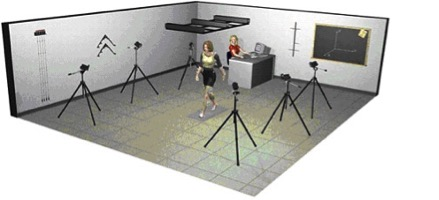
\includegraphics[width=0.9\textwidth]{./graphics/camera}
		\caption{Sistema de medida mediante cámaras} \label{fig:camera}
	\end{figure}
	
	\subsection{Sistemas optoelectrónicos}
	
	Los sistemas optoelectrónicos captan señales luminosas de marcadores colocados en el cuerpo del sujeto a medir y las convierten en señales eléctricas (ver Figura \ref{fig:opt}). A pesar de que se trata de un completo y minucioso método de análisis de la marcha, no resulta muy práctico en el ámbito del análisis clínico. Al alto coste y complejidad del equipo hay que añadir el amplio espacio de trabajo necesario para mantener una línea de visión libre de obstáculos entre el sujeto y los sistemas de medida. Además, la complejidad y lentitud provocan que resulte tedioso el tomar varias medidas \cite{begona,opt}.
		\begin{figure}[H]
			\centering
			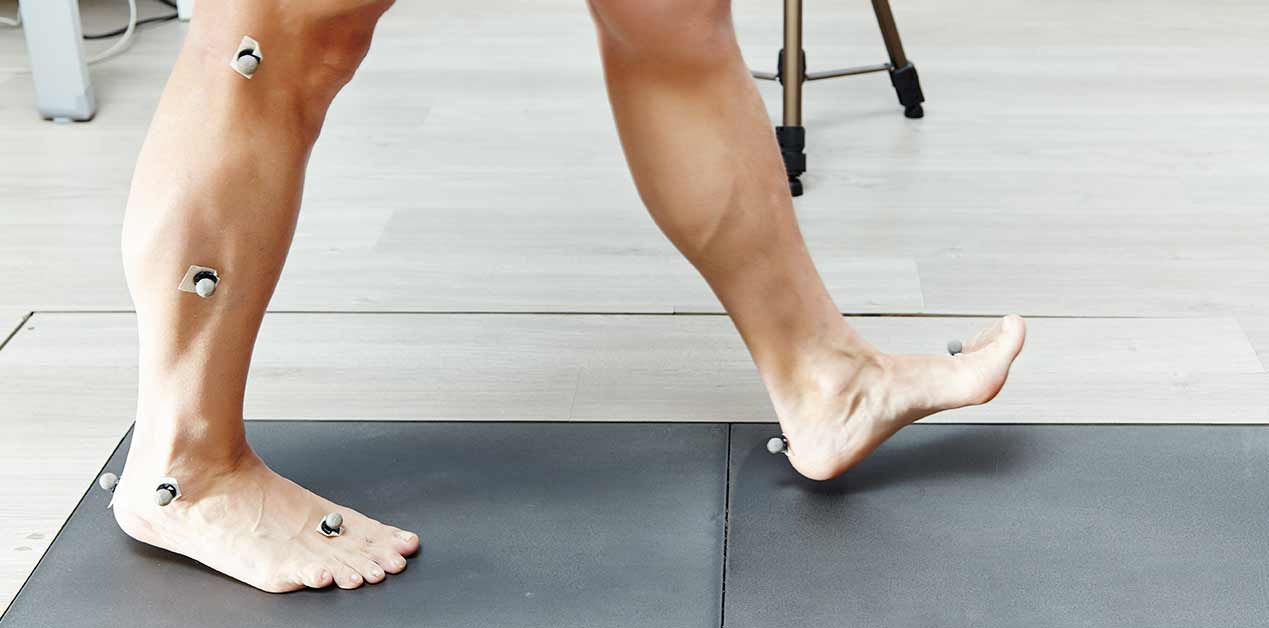
\includegraphics[width=0.9\textwidth]{./graphics/opt}
			\caption{Sistema de medida optoelectrónico} \label{fig:opt}
		\end{figure}

	\subsection{Tapices instrumentados}
	
	Existen sistemas como el GaitRite\textsuperscript{\textregistered} que permiten la medida de diferentes parámetros de la marcha, entre ellos la medida de distancia entre pasos \cite{gaitrite}. En la Figura \ref{fig:gaitrite} se observa dicho sistema el cual consiste en un tapiz instrumentado. Tiene como ventaja la portabilidad y la facilidad de manejo, así como el ahorro de tiempo debido a la automatización en el cálculo de los parámetros obtenidos. Sin embargo, existen ciertas limitaciones, dado que sólo se
	obtiene información de la presión ejercida sobre los sensores, sin tener en cuenta la
	dirección ni las componentes del vector de fuerza \cite{begona}. 
	
	\begin{figure}[H]
		\centering
		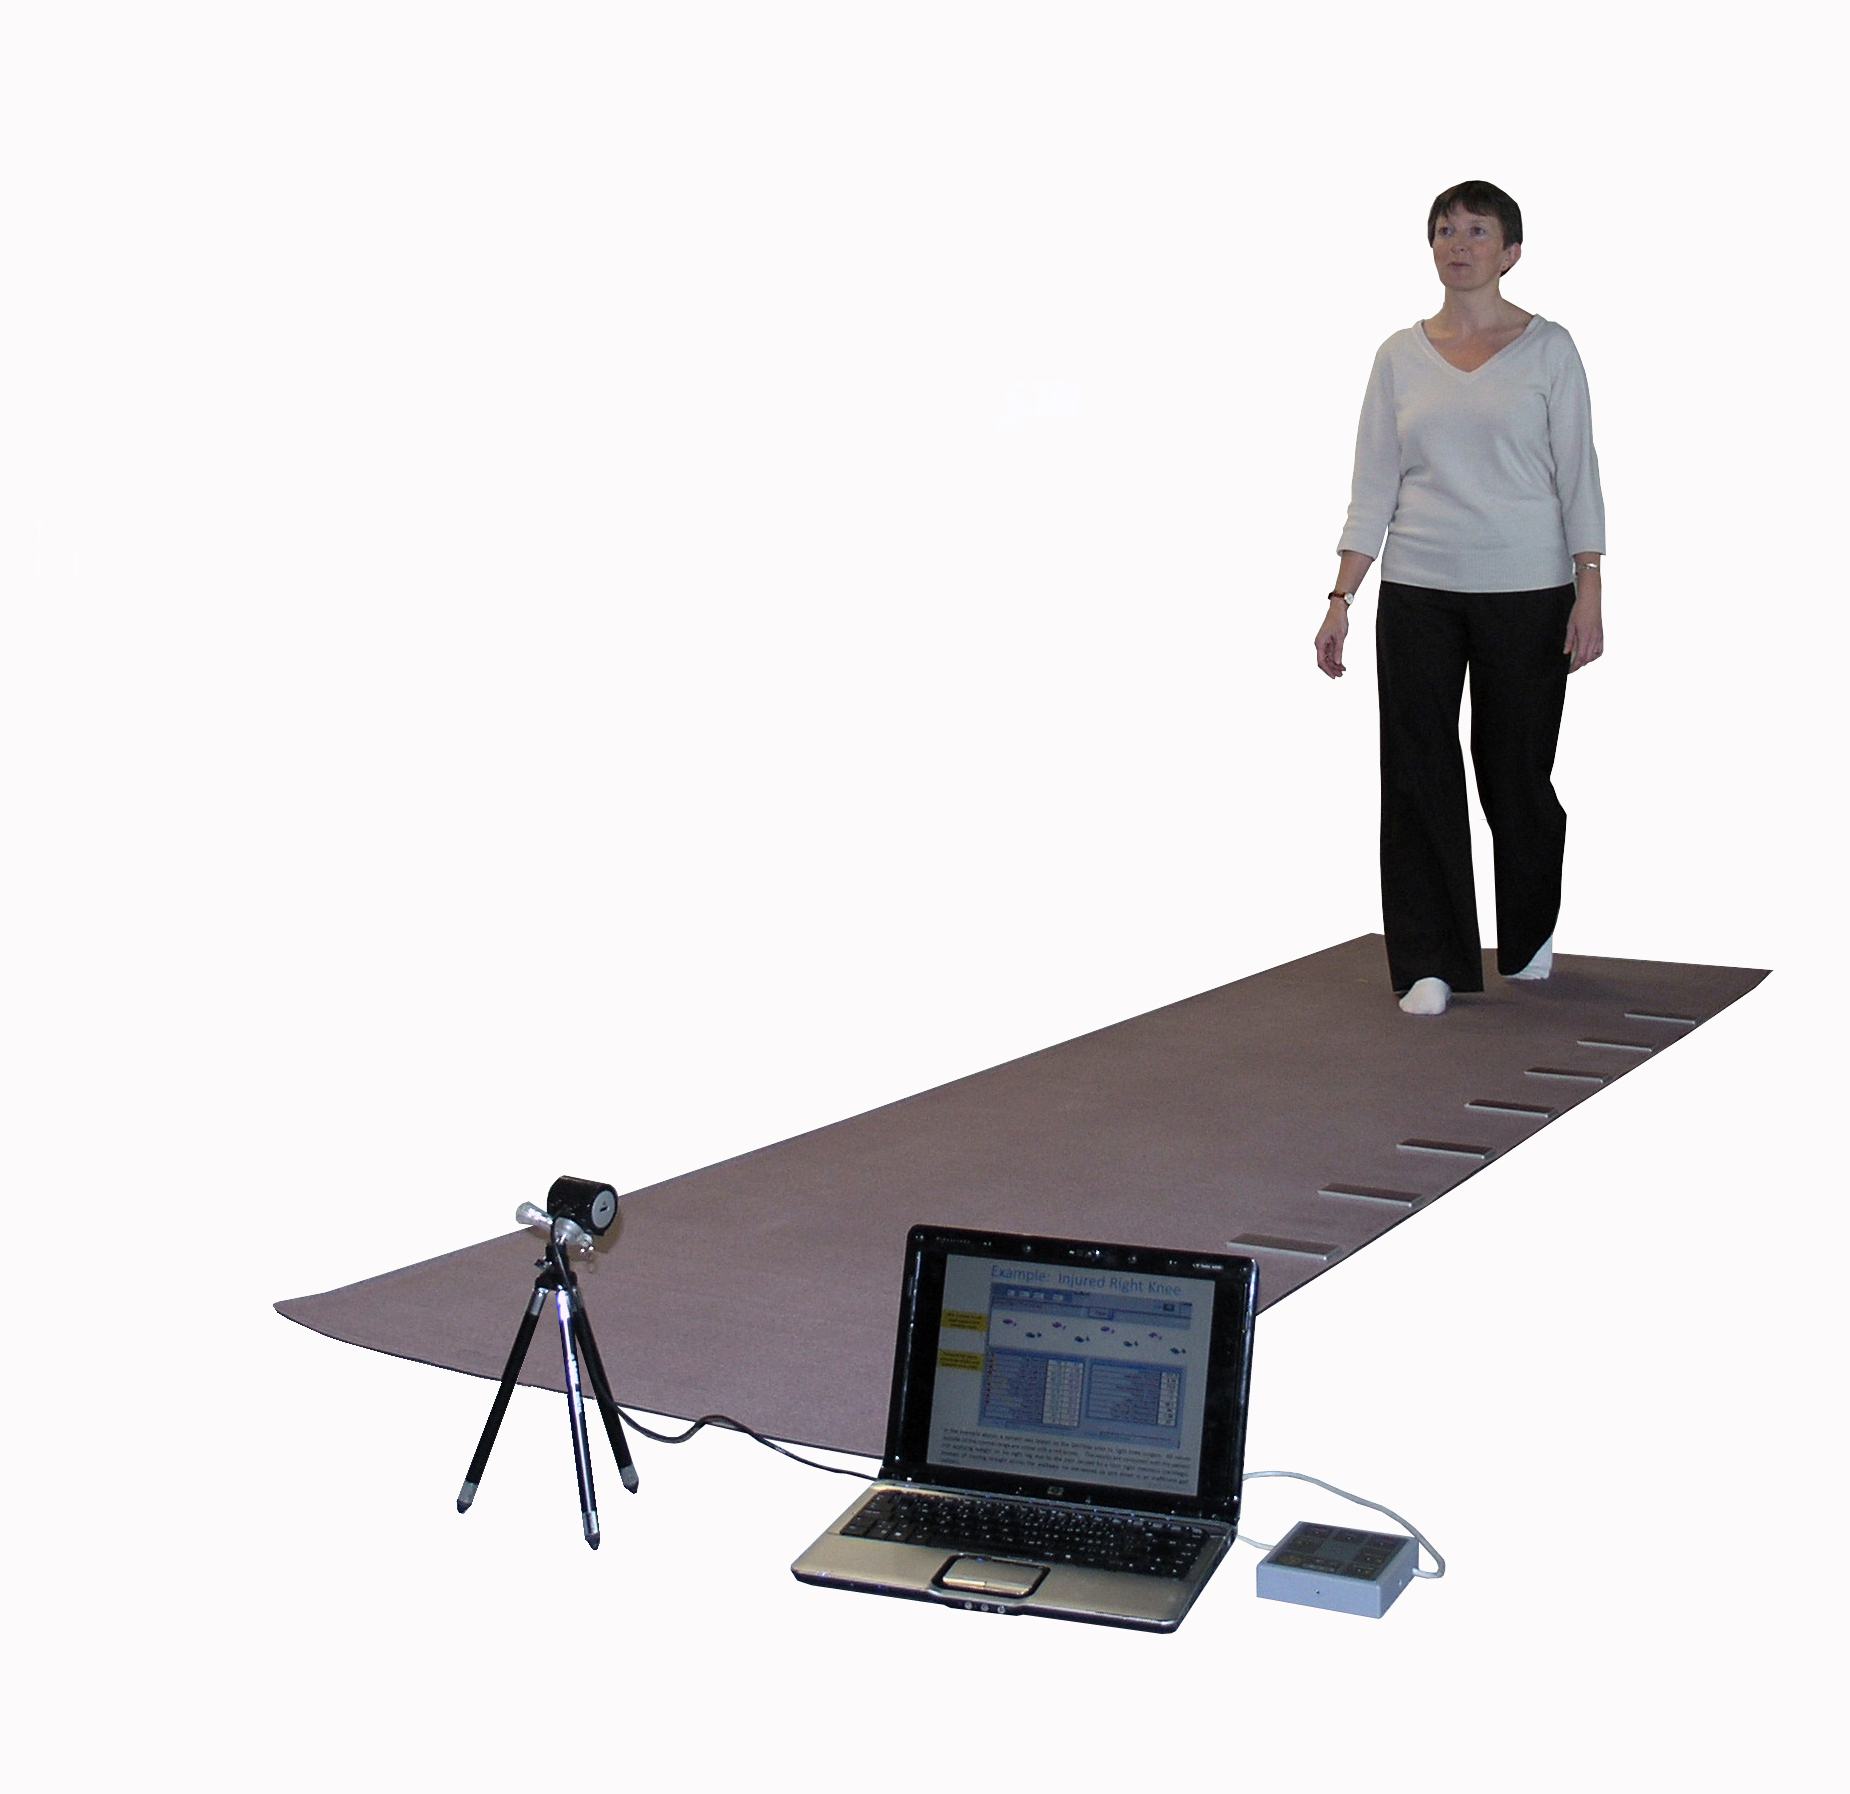
\includegraphics[width=0.6\textwidth]{./graphics/GaitRite}
		\caption{Sistema de medida GaitRite\textsuperscript{\textregistered}} \label{fig:gaitrite}
	\end{figure}
	
	\subsection{Zapatos instrumentados}
	
	\cite{shoes} Existe un sistema de medida integrado en zapatos que combina la utilización de sensores inerciales así como sensores de fuerza que completan la medida de los parámetros de la marcha. Se trata de un diseño compacto y que puede ser utilizado en entornos diferentes. En la Figura \ref{fig:shoes} aparece representado el diseño del zapato utilizado.
	
		\begin{figure}[H]
			\centering
			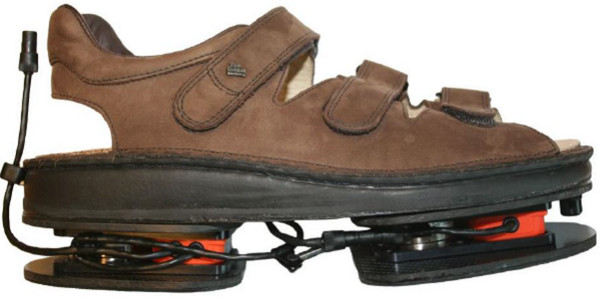
\includegraphics[width=0.6\textwidth]{./graphics/shoes}
			\caption{Zapatos instrumentados} \label{fig:shoes}
		\end{figure}
		 

Cada uno de los zapatos tienen un peso de aproximadamente 1.1Kg por lo que pueden afectar en la marcha a los pacientes ya que existe gran probabilidad de que hayan perdido fuerza en alguno de los lados. Además, únicamente con estos zapatos no es posible el cálculo de la distancia entre pasos por lo que aparecen nuevas versiones en las que se añaden sensores de ultrasonidos y por tanto reducen la ergonomía del sistema  \cite{shoes} . 


	
	
	
\thispagestyle{empty}
%
% Diseño
%
%\chapter{Desarrollo del proyecto\label{sec:disenho}}

Para la realización de este trabajo se han tomado dos de las tecnologías expuestas en el capítulo \ref{sec:estado_del_arte} y se han llevado a la práctica. De esta manera se puede trabajar empíricamente con dos tecnologías diferentes planteadas como solución para un mismo problema. Una vez realizado todo el trabajo experimental se puede proceder a evaluar las características prácticas de cada tecnología y compararlas entre ellas. 

En función de la tecnología en que la se apoya cada uno de las soluciones, %por un lado se estudian los sensores de fibra FBG, capítulo \ref{sec:FBG3}, y por otro lado, los sensores IMU, capítulo \ref{sec:IMU3}.  
este capítulo se estructura de la siguiente manera: 
\begin{itemize}
	\item {\textbf{\ref{sec:FBG3}}    .- Solución con sensores de fibra FBG} 
	\item {\textbf{\ref{sec:IMU3}}    .- Solución con sensores IMU}
\end{itemize}




Dentro de cada punto se detalla toda la información necesaria para la implementación de cada uno de los sistemas. En ambos casos, la exposición de la solución tomada se divide en la explicación teórica en el \textit{Marco conceptual} y el ensayo práctico en el \textit{Desarrollo del prototipo}. El desarrollo del prototipo estudia los materiales empleados, el proceso de fabricación y el funcionamiento.  

%------------------------------
%------___SOLUCIÓN_FBG___------
%------------------------------
\section{Solución con sensores de fibra FBG}
\label{sec:FBG3}

\textcolor{rositaoscuro}{
	\textit{
		\colorbox{yellow}{Introducción} breve del guante, que tecnologias implica.
		Resumen fibras de Bragg 
		¿Qué es una fibra FBG?
		¿Porque se utilizan?
		El procesado de las señales resultantes se realiza mediante Labview.
	}
}


 Como primer prototipo se ha estudiado y llevado a cabo un guante cuyo funcionamiento se basa en los sensores de fibra FBG. 
 
 El prototipo consiste en una sección de PDMS con forma de huella de mano que tiene embebida una red en fibra de Bragg. Para la obtención, procesado y visualización de los resultados medidos se emplea el entorno de desarrollo LabVIEW.


%--Marco conceptual
\subsection{Marco conceptual}
\label{sec:mc3FBG}

Este apartado tiene por finalidad realizar una clara exposición de los conceptos teóricos fundamentales para la comprensión del diseño llevado a cabo. 

\begin{itemize}
%--FIBRA ÓPTICA
	\item \textbf{Fibra óptica}
	
	\textcolor{rositaoscuro}{
		\textit{
			Cómo se propaga la luz en ella.\\
	 		- -Partes de la fibra.\\
			Tipos de emisores (LED Laser).\\
			Receptores.\\
			Conectores.\\
			- -Fabricación.\\
			Soldado.\\
			- -Tipos de fibra.\\
		}
	}

	La fibra óptica es una hebra de material dieléctrico, así cómo el vidrio (sílice) o el polímero acrílico. 
	Se emplea como medio de propagación de señales luminosas. Es decir, para transmitir ondas electromagnéticas del espectro óptico: regiones espectrales de infrarrojo, luz visible y ultravioleta. En la siguiente imagen (figura \ref{fig:espectroOptico}) se puede observar dentro del espectro electromagnético dónde se sitúa el espectro óptico.	 
	\begin{figure}[H]
		\centering
		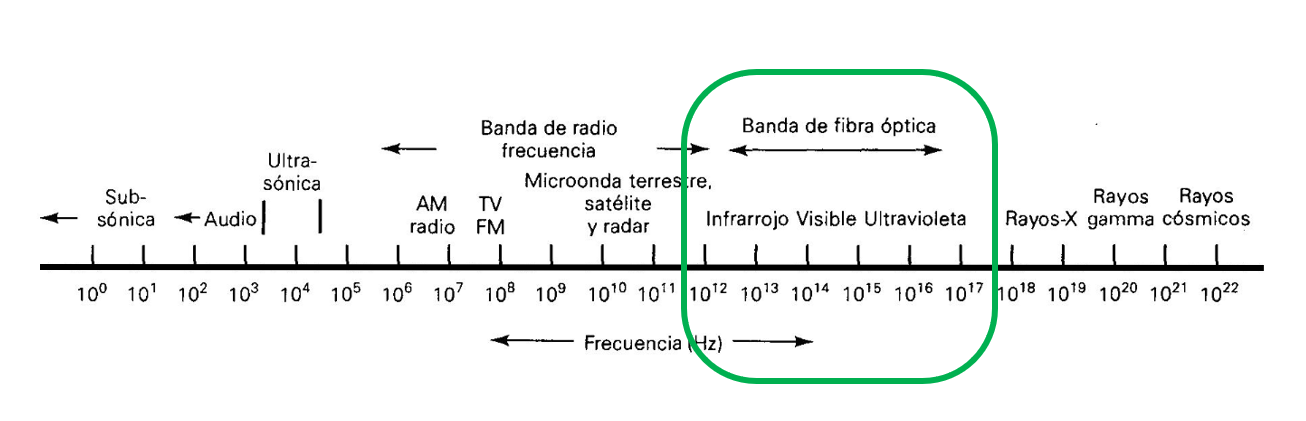
\includegraphics[width=0.95\textwidth]{./img/espectrooptico}
		\caption{Espectro electromagnético en frecuencia.}
		\label{fig:espectroOptico}
	\end{figure}

	Cabe destacar que dentro del espectro óptico las longitudes de onda habituales para comunicación en fibra óptica están entre los 700nm y 1600nm. Estas se dividen en rangos con mejores características para la transmisión, denominadas ventanas de comunicación. Como se muestra en la figura \ref{fig:ventanaOptica}, son tres las ventanas más utilizadas,\cite{ventanasFO}:
%	\begin{itemize}
%		\item \textbf{1ª ventana}\hspace{0.2cm} 800 a  900 nm tilizada  =  850nm
%		\item \textbf{2ª ventana}\hspace{0.1cm}  1250 a 1350 nm   l utilizada  = 1310nm
%		\item \textbf{3ª ventana}\hspace{0.1cm}  1500 a 1600 nm   l utilizada  = 1550nm 
%	\end{itemize}
	
	\begin{table}[H]
		%\centering
		\hspace{2cm}
		\renewcommand{\arraystretch}{2}
		\begin{tabular}{rrl}
			\textbf{1ª ventana}& 800 a  900 nm  & $\longmapsto$ $\,$ longitud de onda utilizada = 850nm  \\
			\textbf{2ª ventana}& 1250 a 1350 nm & $\longmapsto$ $\,$ longitud de onda utilizada = 1310nm  \\
			\textbf{3ª ventana}& 1500 a 1600 nm & $\longmapsto$ $\,$ longitud de onda utilizada = 1550nm   \\ 
		\end{tabular} 
	\end{table}

	 \begin{figure}[H]
	 	\centering
	 	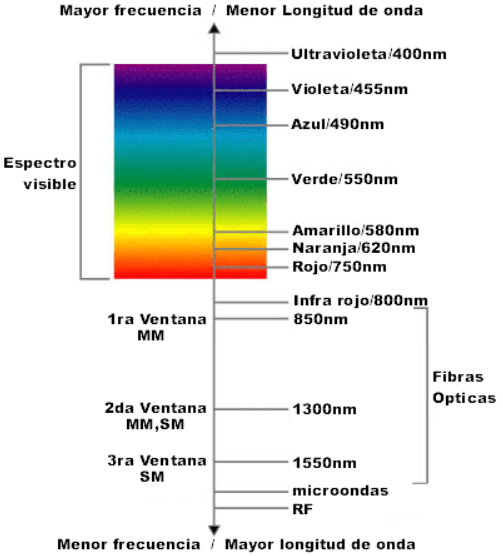
\includegraphics[width=0.5\textwidth]{./img/ventana}
	 	\caption{Longitud de onda fibra óptica junto con el espectro visible. \cite{ventanasFO}}
	 	\label{fig:ventanaOptica}
	 \end{figure}
 
 En cuanto a las propiedades físicas de la fibra óptica, son bastante delicadas ya que su grosor no supera por mucho al diámetro del cabello humano y se obtiene de la extrusión del sílice, SiO\textsubscript{2} , es decir, se trata de un filamento de vidrio muy fino. Es por ello que es la fibra óptica estándar está rodeada de una cubierta protectora. 
 
  \begin{figure}[H]
  	\centering
  	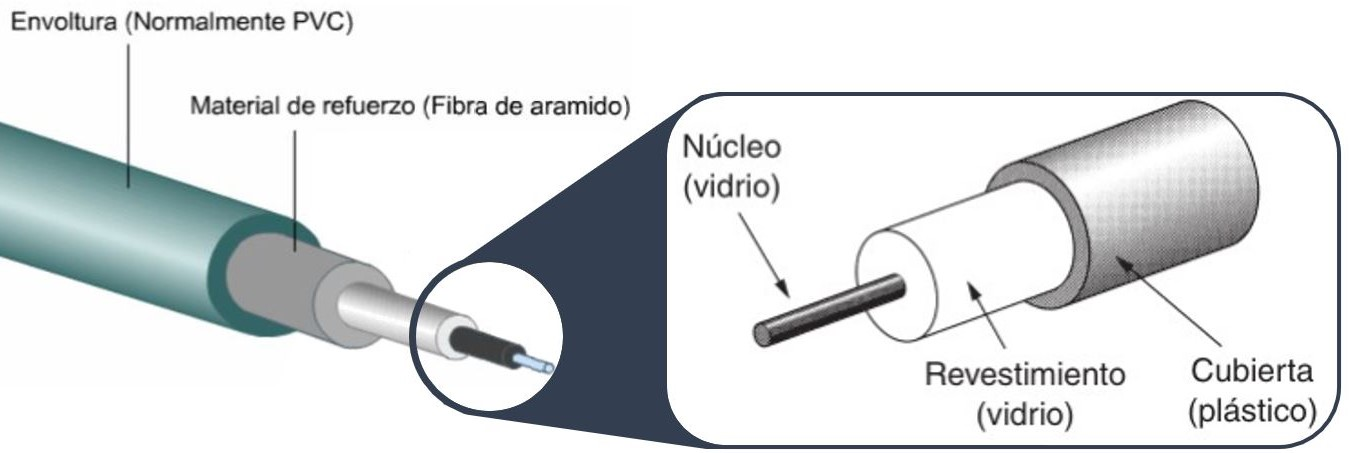
\includegraphics[width=0.87\textwidth]{./img/capas-fibra2}
  	\caption{Capas fibra óptica \cite{imgNucleoFibra,imgCapasFO}} 
  	\label{fig:capasFibra}
  \end{figure} 
  
  
  
 La fibra óptica estándar cuenta varias capas (figura \ref{fig:capasFibra}): núcleo, revestimiento y cubierta (o buffer).  Si la aplicación lo permite, conviene proteger la fibra con más capas externas. En la imagen anterior la fibra está además protegida por un material de refuerzo (fibra de aramido) y una envoltura (PVC).
 
 Tanto el núcleo cómo el revestimiento forman el medio por el cual se propaga la luz. Estas dos capas son tan finas que forman un filamento flexible, pero muy delicado, puesto que es muy propenso a romperse ante dobleces u otras manipulaciones externas. Por ello el resto de las capas son tambien importantes por proporcionar a la fibra protección y haciendo posible su utilización es escenarios de despliegue.
 
 La fabricación de la fibra óptica es un proceso de alta tecnología. Es importante mantener la pureza y la regularidad del núcleo. Esto es complejo, puesto que estamos hablando en algunos casos de núcleos de un grosor entorno a las 8 micras (en fibras monomodo). El grosor estándar de la fibra es de 125 micras(una micra equivale a una millonésima parte de un metro). Para conseguir este resultado el proceso de fabricación consiste en reproducir a escala macroscópica la estructura de la fibra que se quiere obtener. Esta reproducción a gran escala de la fibra deseada se le denomina preforma. Una vez se tiene la preforma, esta se va fundiendo y estirando hasta alcanzar el filamento del diámetro deseado. De una preforma se pueden sacar kilómetros de fibra. Para fabricar la preforma se parte de una barra de vidrio hueca (el vidrio que formará el recubrimiento) y se baña en un gas que contiene unas partículas (lo que formará el núcleo). Al calentar a mil grados, las partículas comienzan a fundirse hasta que el tubo colapsa y forma una vara maciza, que es la preforma. Para fundirla y estirarla esta se coloca verticalmente y se calienta. La complejidad de esta fase reside en mantener constante el flujo y el diámetro del hilo resultante. Además durante esta fase se aprovecha para crear una capa protectora sobre el vidrio (cubierta en la figura \ref{fig:capasFibra}). Finalmente los kilómetros de fibra óptica se enrollan en grandes bobinas. \cite{fabricacionFO}
 
  \begin{figure}[H]
 	\centering
 	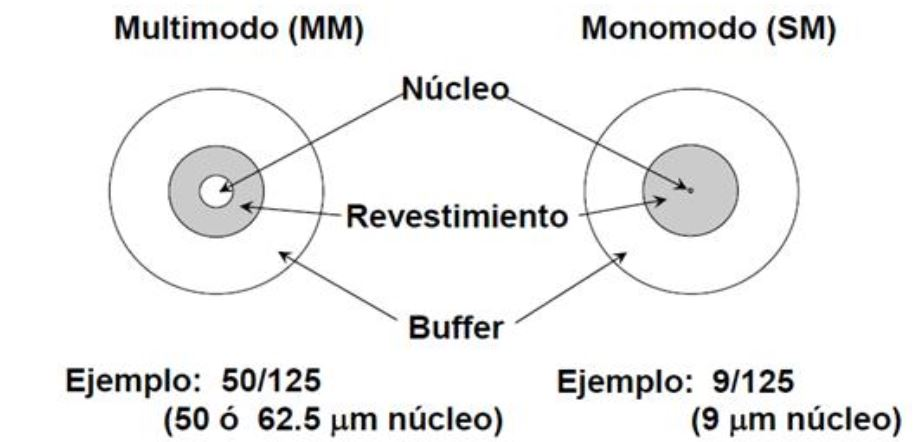
\includegraphics[width=0.6\textwidth]{./img/MM-SM}
 	\caption{Relación grosor fibra multimodo (MM) y monomodo (SM) \cite{imgRadioModo} } 
 	\label{fig:modoMonoMulti}
 \end{figure} 
 
  Dependiendo de la relación de diámetro entre el núcleo y el revestimiento, la fibra fibra será monomodo o multimodo (figura \ref{fig:modoMonoMulti}). Esta diferencia afecta a la propagación de la luz dentro de la guía de onda. Ya se ha comentado que el diámetro de la fibra es de aproximadamente 125 micras. En el caso de las fibras monomodo, el núcleo de estas tiene un diámetro tan pequeño (en torno a 8 micras) que la luz solo puede propagarse en un sólo modo (rayo). Sin embargo, en el caso de las fibras multimodo, al poseer un núcleo mayor (entre 50 o 62.5 micras) soportan la transmisión el múltiples modos, es decir, los rayos de luz viajan en muchas direcciones a través de este. \cite{FOA} 
   
  	\textcolor{rositaoscuro}{revisar:}
 	\begin{figure}[H]
		\centering
		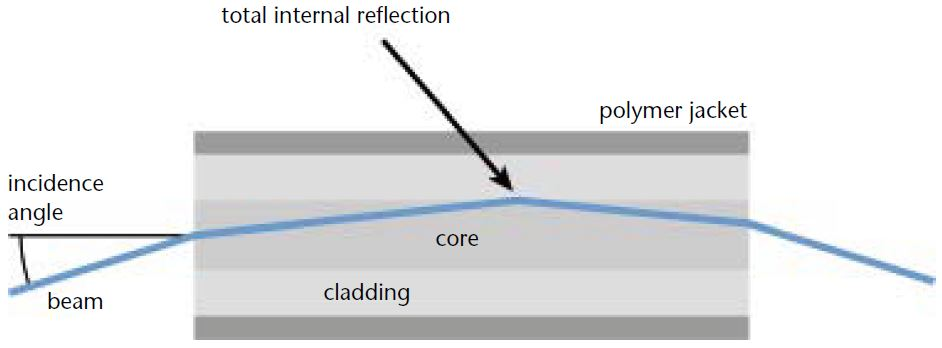
\includegraphics[width=0.5\textwidth]{./img/guiaMM}
		\caption{Guía de un haz de luz en una fibra multimodo a través de la reflexión interna total en la interfaz núcleo-revestimiento. \cite{imgMonoMulti} } 
		\label{fig:guiaMM}
	\end{figure} 
  	\begin{figure}[H]
		\centering
		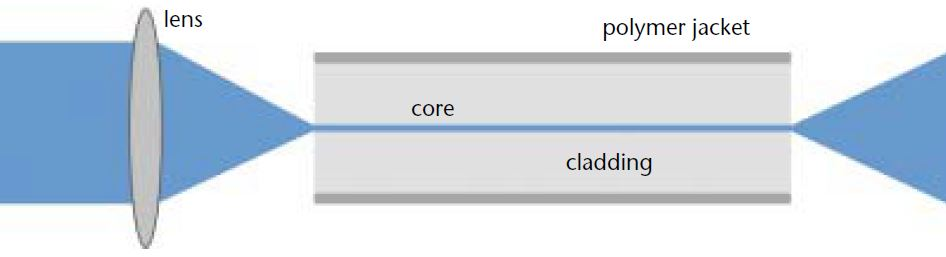
\includegraphics[width=0.7\textwidth]{./img/guiaSM}
		\caption{Orientación de la luz en una fibra monomodo. El perfil de intensidad dentro del núcleo está determinado únicamente por el diseño de la fibra. \cite{imgMonoMulti} } 
		\label{fig:guiaSM}
	\end{figure}  
 	
 	\textcolor{rositaoscuro}{\textit{Si veo que tal puedo extenderme con relacionar las \underline{ventanas con monomodo y multimodo}. Y además concretar mas las \underline{características de cada ventana} (gráfica de interferencias esta)}\\
 	\\Generalmente, la fibra multimodo se utiliza con fuentes LED en longitudes de onda de 850 y 1300 nm (ver debajo) para redes de área local (LAN) más lentas y con fuentes láser a 850 nm (VCSEL) y 1310 nm (láser Fabry-Perroy) para redes que operan a velocidades de gigabits por segundo o mayores. \\
	La fibra monomodo se utiliza para telefonía y para televisión por cable (CATV) con fuentes de luz láser a 1300 y 1550 nm ya que tiene poca pérdida y un ancho de banda prácticamente infinito.\\
	Existen otros tipos de fibras opticas: POF - PCS y HCS (imagen ejemplo de diámetros).}

 La diferencia de índices de refracción entre las capas centrales de la fibra son las que permiten la propagación de la luz a través de esta. El índice de refracción del núcleo es mayor que el del revestimiento.
 
\cite{geometriaBasicaFP}
 
 
 
  \textcolor{rositaoscuro}{//explicar más REFRACCIÓN}

  Puesto que en la solución con estudiada en este trabajo se utilizan fibras monomodo no se va a extender el texto en explicar más conceptos sobre la transmisión en fibras multimodo.
 
 
 Los sistemas de propagación de señales luminosas a través de la fibra óptica componen un medio de transmisión de datos rápido y fiable. Previa a la propagación a través de un medio óptico de una señal eléctrica (analógica o digital) es necesario realizar una conversión de esta a señal óptica. Esto genera una señal óptica a partir de una señal eléctrica en el emisor o fuente de luz situado en el extremo inicial de la comunicación. Realizada la conversión, la señal es transmitida a lo largo de la fibra óptica. Según las características del escenario puede haber una o varias uniones entre fibras a lo largo del canal. Estás pueden realizarse empalmando o utilizando conectores. Una vez la señal óptica atraviesa todo el canal, llega al detector, dónde sucede el proceso inverso al ocurrido en el emisor y a la salida del sistema completo se tiene la señal eléctrica. Esta corresponde a la señal introducida al sistema con una pequeña posibilidad de haber sufrido pérdidas o atenuación debido a la impureza de la fibra, la distancia, las conexiones entre elementos del sistema o cualquier otro evento ajeno al este. Estas modificaciones de la señal de entrada pueden ser contrarrestadas o solventadas en recepción sin suponer un impedimento a una comunicación exitosa. (figura \ref{fig:TxFOp2p})
 
   \begin{figure}[H]
 	\centering
 	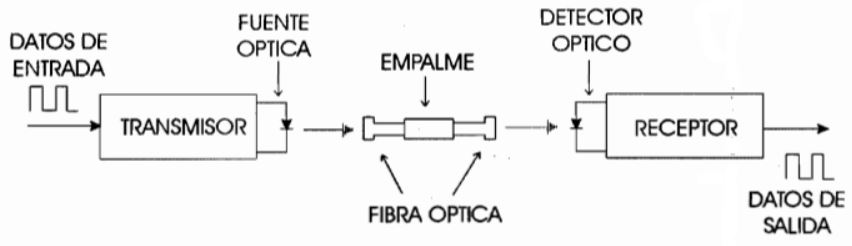
\includegraphics[width=0.75\textwidth]{./img/TxFOp2p}
 	\caption{Transmisión punto a punto de señales a través de fibra óptica. \cite{txFO} } 
 	\label{fig:TxFOp2p}
 	\end{figure} 

 Veamos por separado los elementos dibujados en la figura \ref{fig:TxFOp2p}:
 	\begin{itemize}
 		\item \textit{\textbf{Emisores (Transmisión)}}	
 		% \hspace{0.2cm} 
 		
 		\item \textit{\textbf{Detectores (Recepción)}}
 			
 			
 		\item \textit{\textbf{Conectores y empalmes}}
 		
 	 \end{itemize}
 


					//--\\						
					La propagación de la luz desde el punto inicial hasta el extremo final se debe al fenómeno de
					reflexión total interna [20] de la luz. Este hecho tiene lugar cuando un haz de luz trata de
					pasar de un medio de mayor índice de refracción, n1, a uno de menor índice de refracción, n2,
					y con un ángulo determinado (Fig. 3.3.). El ángulo de incidencia debe superar el valor crítico.
					Cuando se dan estas condiciones, el rayo de luz incidente se refleja completamente, no
					pudiendo atravesar la frontera que separa ambos medios y volviendo nuevamente hacia el
					medio origen, con un ángulo de reflexión igual al ángulo de incidencia.
					
					
					En una fibra óptica, para provocar el fenómeno de reflexión total interna, se asegura que la luz
					penetra con una determinada apertura numérica, que es el ángulo necesario para forzar a la
					mayoría de los rayos de luz a incidir sobre la superficie de separación entre el núcleo y la
					cubierta. En estas condiciones, y de acuerdo con las leyes de Snell, los rayos de luz incidentes
					a esta interfaz de separación superan el ángulo crítico, pudiendo así reflejarse prácticamente
					en su totalidad a lo largo de toda la estructura.
					


---

TIPOS DE EMISORES


					///---
					LASER
					
					Para poder transmitir en una de estas ventanas es necesaria una fuente de luz "coherente", es decir de una única frecuencia (o longitud de onda), la cual se consigue con un componente electrónico denominado LD ó diodo LASER (Light Amplification by Estimulated Emision of Radiation). Este componente es afectado por las variaciones de temperatura por lo que deben tener un circuito de realimentación para su control.
					
					También pueden usarse diodos LED.
					
					Detectores ópticos
					
					Como receptores ópticos se utilizan fotodiodos APD o diodos pin (PIN-PD) que posen alta sensibilidad y bajo tiempo de respuesta.
					
					El APD también requiere de un ajuste automático ante variaciones de temperatura.


\textcolor{teal}{
	Recubrimientos: http://apacoe.weebly.com/conocimiento/que-es-la-fibra-optica
	Link:Conectores y empalmes
	http://www.thefoa.org/ESP/Conectores.htm
}

%-- REDES DE DIFRACCIÓN DE BRAGG	
	\item \textbf{Redes de difracción de Bragg}
		
	Funcionamiento y sensibilidad
	
%-- POLIDIMETILSILOXANO - PDMS	
	\item \textbf{Polidimetilsiloxano (PDMS)}
		
	Material empleado para embeber las FBGs.
	
%-- LABVIEW 	
	\item \textbf{LabVIEW}
		
	LabVIEW es un software de ingeniería de sistemas que requiere pruebas, medidas y control con acceso rápido a hardware e información de datos. \cite{LabVIEWpage}





\end{itemize}
 
%--Desarrollo del prototipo
\subsection{Desarrollo del prototipo}
\label{sec:prot3FBG}
%[Esta parte de desarrollo del proyecto parte de otro trabajo. Aquí mencionar algo que diga el trabajo de Silvia y mencionar la en la bibliografía.]

La realización del primer desarrollo se origina a partir de un trabajo realizado con anterioridad en el grupo de investigación de la universidad\cite{SilviaTFM}. Se mejora el soporte físico(hardware) y se desarrolla un nuevo programa con un interfaz de usuario simple e intuitivo.

El prototipo consiste en un prototipo técnico y funcional de un guante, con sensores de FBG embebidos en PDMS. 
 
\subsubsection{Materiales}
En este apartado se disponen brevemente los componentes utilizados para el 
\begin{figure}[H]
	\centering
	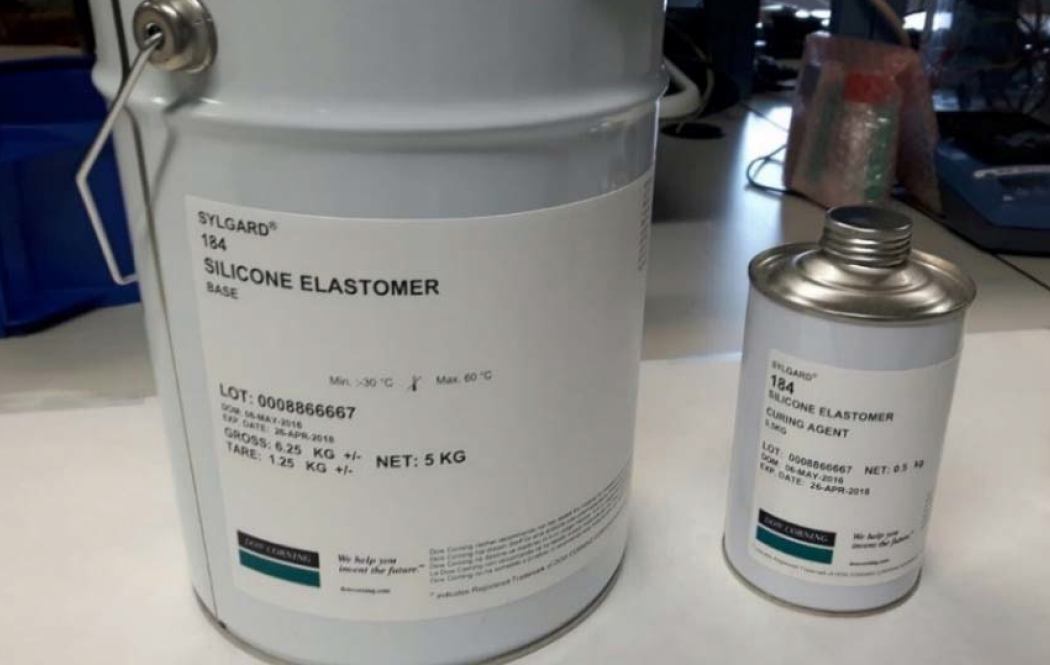
\includegraphics[width=0.75\textwidth]{./img/PDMS}
	\caption{PDMS: Elastómero y agente de cura.} \label{fig:pdms}
\end{figure}



\subsubsection{Proceso de fabricación del soporte físico}
%Elaboración
Para que sea más cómoda la explicación del proceso de elaboración del prototipo se divide este en tres partes: modelado 3D, fabricación del guante y montaje de prototipo completo.

\begin{itemize}
	\item \textbf{Modelado 3D - Configuración 3D}
	
	Esta actividad comprende el diseño del molde con el que se fabrica el guante y de la caja contenedora de todo el cableado.
	Para poder producir el guante de PDMS es necesario tener un molde donde verter la disolución para darle la forma deseada. Gracias a las versatilidad de diseño que ofrece la impresión 3D se realiza con este proceso de manufactura el molde (véase figura \ref{fig:molde}). 
\begin{figure}[H]
	\centering
	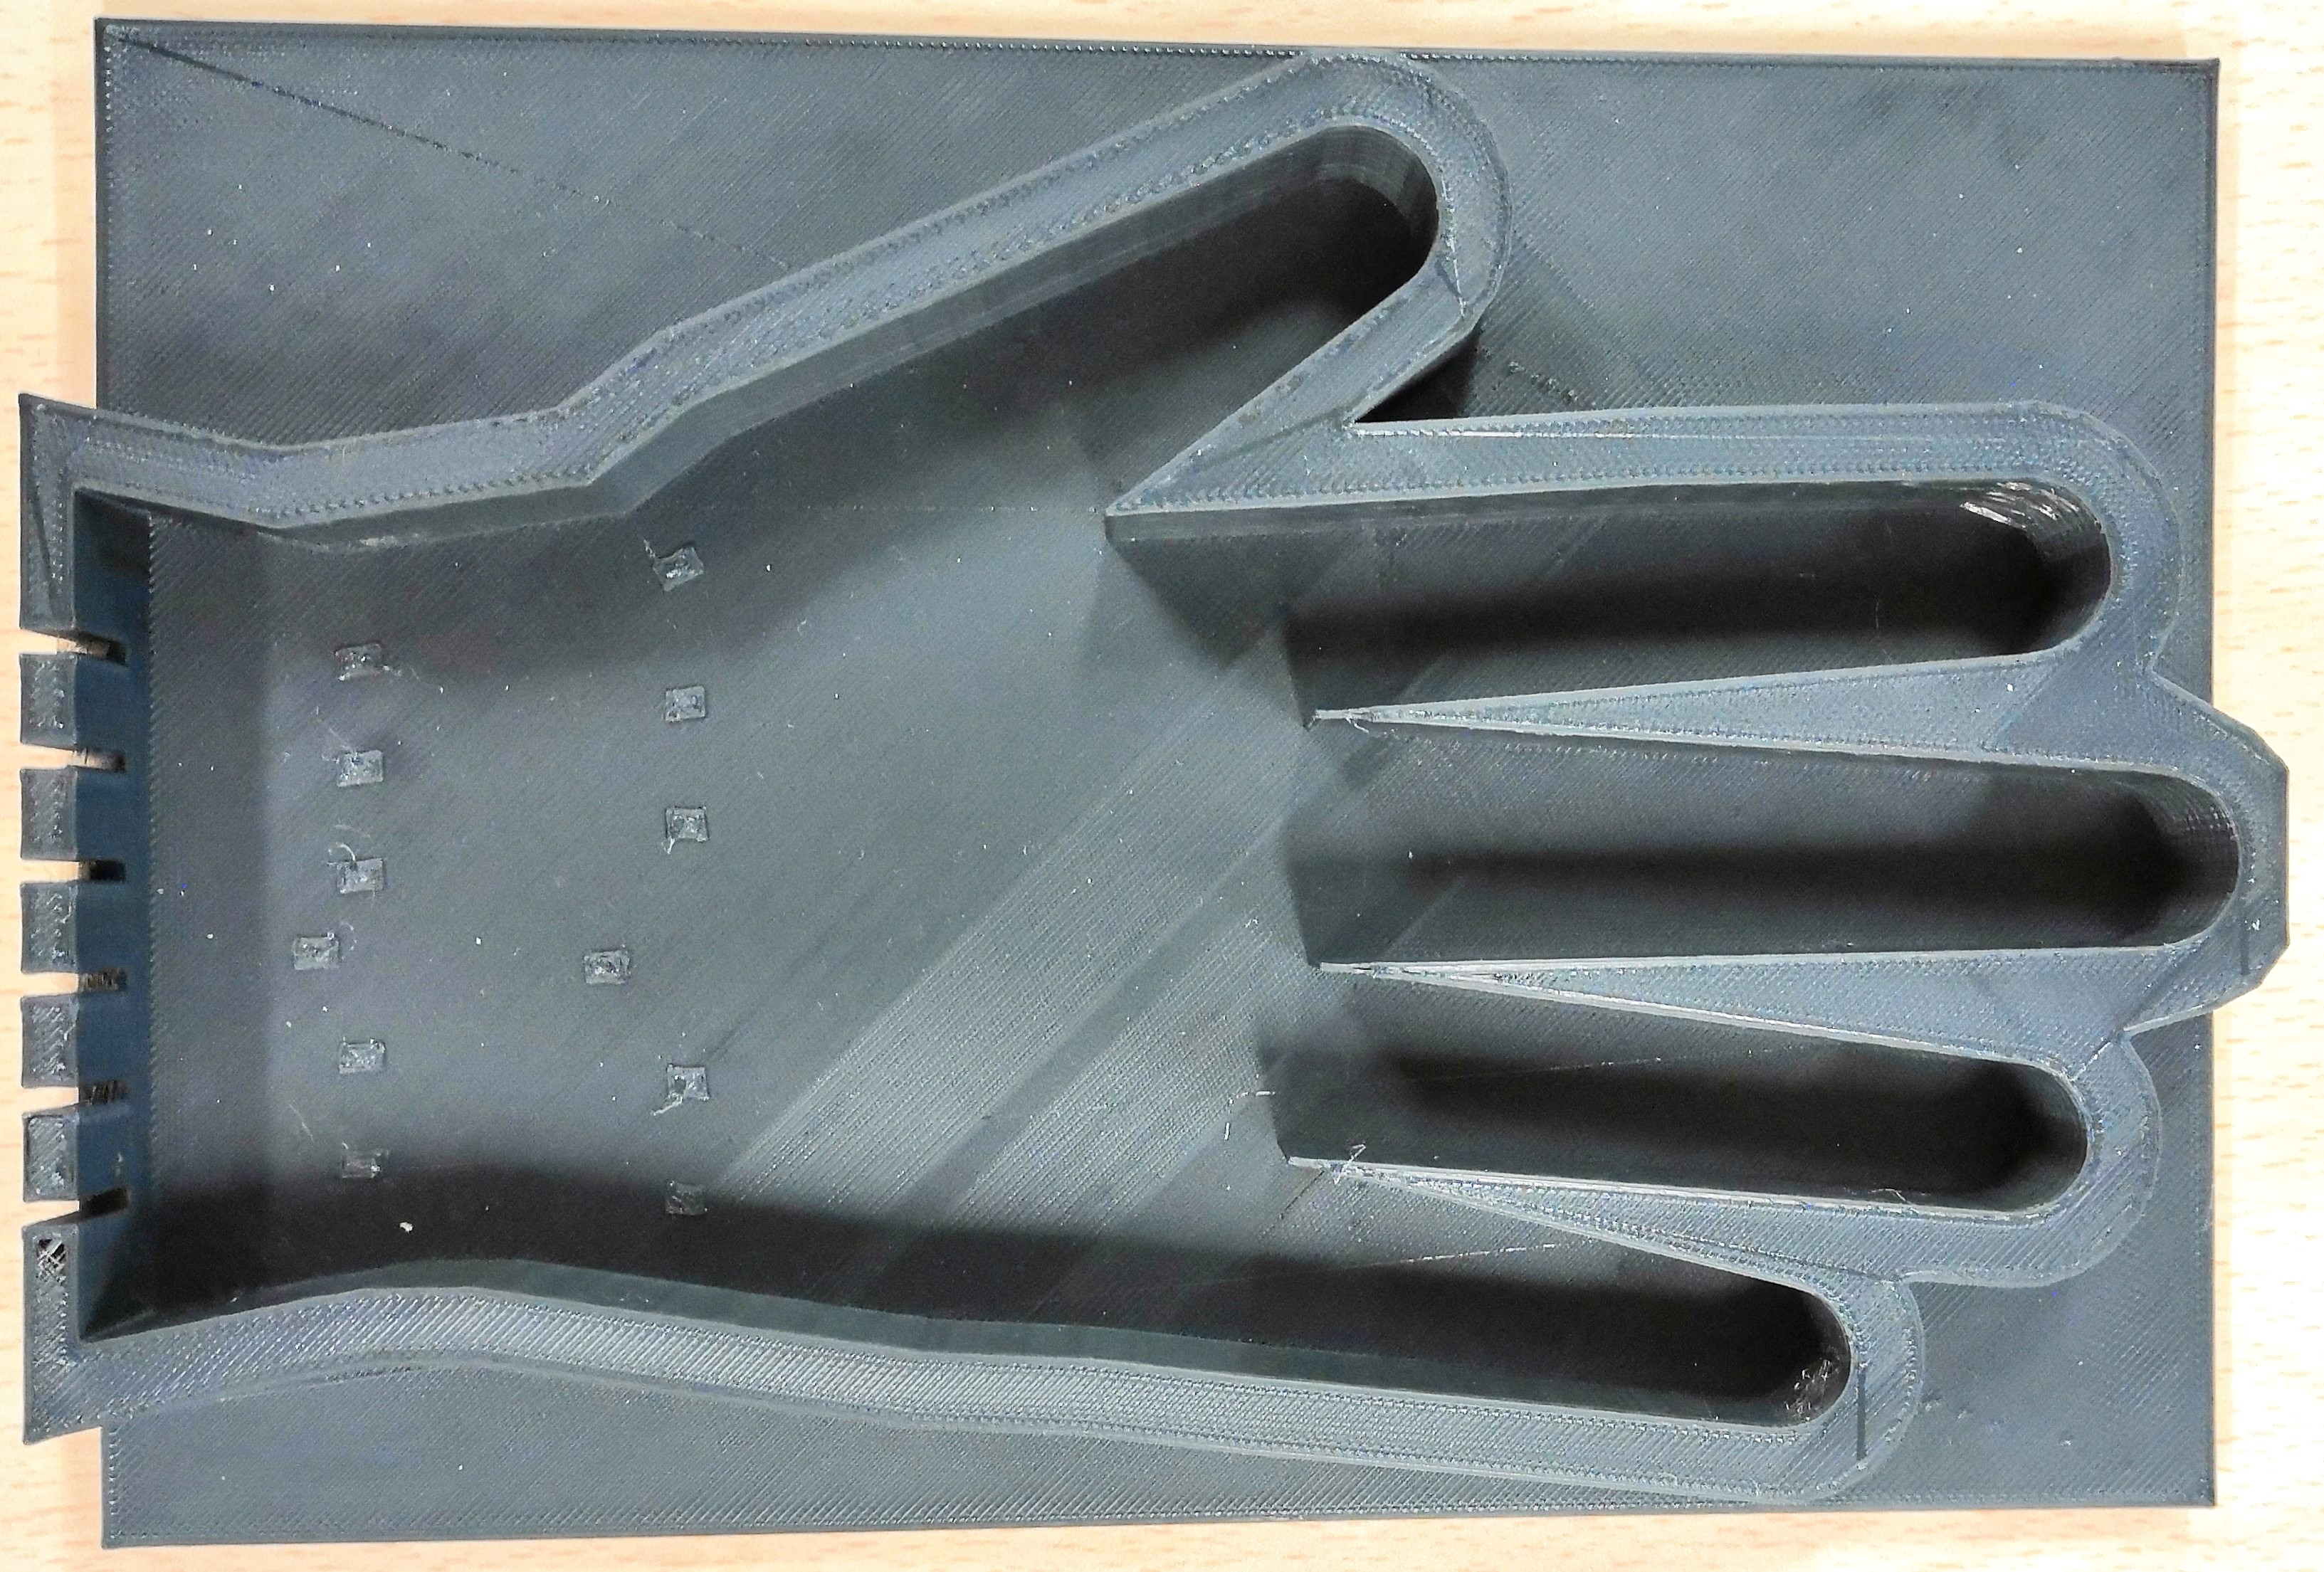
\includegraphics[width=0.5\textwidth]{./img/molde1}
	\caption{Molde} \label{fig:molde}
\end{figure}

	
 
	\item \textbf{Fabricación del guante}
	
	Para el proceso de fabricación del guante se necesitan ..................
	
	\begin{enumerate}
		\item Preparar mezcla PDMS (35g de polímero y 3.5g de agente de curación). Primero el
		elastómeto y después agente de curación.
		\item Revolver la mezcla durante al menos 4 minutos.
		\item Se deposita el PDMS y se colocan las fibras en el molde
		\item Se introduce en un horno de vacío para eliminar las burbujas durante 20 minutos, sin aplicar
		temperatura.
		\item Meter el molde en el horno (4h y media a $-55\,^{\circ}\mathrm{C}$). Dejar un poco más.
		\item Desmoldar.

	\end{enumerate}
	
	
	\item \textbf{Montaje completo}
	
	asdf
	
\end{itemize}

asdf





\begin{table}[H] %BORRAR
	\centering
	\begin{tabular}[t]{|c|}
		\hline
		\textbf{\textcolor{rositaoscuro}{BORRAR}} \\
		\hline
		longitudes de onda del guante de fibras cortas\\
		\hline
	\end{tabular}
	\begin{tabular}[t]{|r|c|}
		\hline
		 & Longitud de onda del sensor\\
		\hline
		\hline
		Dedo pulgar & 1512 nm \\
		\hline
		Dedo índice & 1520 nm \\
		\hline
		Dedo corazón & 1528 nm \\
		\hline
		Dedo anular & 1536 nm \\
		\hline
		Dedo meñique & 1544 nm \\
		\hline
		Muñeca & 1556 nm \\
		\hline
	\end{tabular}
	\caption{Tabla longitud de cada sensor FBG}
	\label{tabla:medidas 80 cm}
\end{table}
%-- Hasta aquí borrar la tabla.


\begin{table}[H]
	\centering
	\begin{tabular}[t]{|r|c|}
		\hline
		& Longitud de onda del sensor\\
		\hline
		\hline
		Dedo pulgar & 1532 nm \\
		\hline
		Dedo índice & 1548 nm \\
		\hline
		Dedo corazón & 1576 nm \\
		\hline
		Dedo anular & 1568 nm \\
		\hline
		Dedo meñique & 1560 nm \\
		\hline
		Muñeca & 1541.26 nm \\
		\hline
	\end{tabular}
	\caption{Tabla longitud de cada sensor FBG}
	\label{tabla:medidas 80 cm}
\end{table}

Para determinar la valid


\subsubsection{Funcionamiento}
asdf

\begin{figure}[H]
	\centering
	\includegraphics[width=1\textwidth]{./img/interfazSM}
	\caption{Interfaz del programa de labview.}
	\label{fig:interfaz}
\end{figure}

%------IIIIIIMMMMMMUUUUUU------
\section{Solución con sensores IMU}
\label{sec:IMU3}
asdf

\subsection{Marco conceptual}
\label{sec:mc3IMU}
asdf

\subsection{Desarrollo del prototipo}
\label{sec:prot3IMU}
asdf

\subsubsection{Materiales}
asdf


\subsubsection{Elaboración/Proceso de fabricación}
asdf

\subsubsection{Funcionamiento}
asdf




\section{---------------}

ME PLENTEO LA POSIBILIDAD DE DIVIDIR EL CAPITULO 3 EN CAPITULO 3 Y 4.


----------------------------------------------------------------------------------------------------------------------------------------------------------------------------------------------------------------------------------------------------------------------------------------------------------------------------------------------------------------------------------------------------------------------------------------------------------------------------------------------------------------------------------------------------------------------------------------------------------------------------------------------------------------------------------------------------------------------------------------------------------------------------------------------------------------------------------------------------------------------------------------------------------------------------------------------------------------------------------------------------------------------------------------------------------------------------------------------------------------------------------------------------------------------------------------------------------------------------------------------------------------------------------------------------------------------------------------------------------------------------------------------


\section{---------------}















En este capítulo se detalla la metodología empleada para el diseño del sistema adaptado al contexto en el que se aplica. Se describe cada uno de los componentes que forman parte del sistema de medición así como el procesado posterior de los datos para obtener la distancia entre pasos(Matlab\textsuperscript{\textregistered}). En el diseño intervienen sensores inerciales (Xsens Technologies B.V, The Netherlands) y se propone el diseño de un sensor de ultrasonido de bajo coste basado en la tecnología Arduino. 


\section{Sistema de medida}
En la Figura \ref{fig:esquema} aparece representado un esquema general de la metodología empleada. Mediante el sensor de ultrasonidos se obtiene la distancia D1 y con los sensores inerciales se obtiene la distancia D2 aplicando a cada una de las señales el procesado que se detallará en posteriores apartados.


Por tanto, el diseño del sistema puede descomponerse en dos niveles de jerarquía  (ver Figura \ref{fig:esquemaniveles}). El primero de ellos, a más bajo nivel, es el diseño del sensor de ultrasonidos y la obtención de las señales necesarias para el cálculo de cada una de las distancias de ambos sensores. El segundo de los niveles es el correspondiente al de la sincronizcación y post-procesado de los datos para determinar la distancia entre pasos.

 Con el  post-procesado de las señales obtenidas por cada uno de los sensores se obtendrán las distancias D1 y D2 que permitirán el cálculo de la distancia objetivo mediante la ecuación \ref{eq:distancia} (Teorema de Pitágoras).

\begin{equation}\label{eq:distancia}
Dist.sep.pasos = \sqrt{D1^2 + D2^2}
\end{equation}


En los siguientes apartados se especifican cada uno de los componentes que intervienen en el sistema. 
\section{Sensores inerciales}
\subsection{Principio de funcionamiento}

Un sistema de referencia inercial se trata de un sistema de referencia regido por las leyes de movimiento de Newton. Por tanto, un sensor capaz de medir valores respecto a dicho sistema de referencia es lo que se conoce como un sensor inercial.

Una unidad inercial o IMU (Inertial Magnetic Unit) es un dispositivo que se compone de tres giróscopos (para determinar la orientación), tres acelerómetros y un reloj que permite asignar tiempo a los valores medidos por los sensores inerciales. Dichas unidades inerciales presentan tres ejes y cada uno de ellos presenta un acelerómetro y un giróscopo.

Por tanto, la información que se recoge de las unidades inerciales son aceleraciones lineales, velocidades angulares y tiempo común para los tres ejes que llevan dicha información de aceleración y velocidad angular (ver Figura \ref{fig:Imu}). 


El tiempo requerido para la implementación del sistema de medida puede influir en la marcha de los pacientes y por tanto en la obtención de los parámetros \cite{begona}. Los sensores inerciales utilizados permiten realizar las mediciones de una manera sencilla y rápida lo cual resulta beneficioso en el contexto ambulatorio tanto para los pacientes como para el personal sanitario



\subsection{Sensores inerciales propuestos}
Los sensores inerciales utilizados para el sistema son el modelo MTw Awinda (Xsens Technologies B.V, The Netherlands) pueden verse representados en la Figura \ref{fig:sensor_XSENS}



Su tamaño es de 47 x 30 x 13mm y 16g de peso por lo que puede definirse como un sistema compacto y ergonómico que será de utilidad para el sistema propuesto en este trabajo. Dispone de unas bandas de sujeción que permiten colocar el sensor en el lugar necesario y por tanto dota de versatilidad al diseño. 

Además, se incluye un software de captura que resultará útil para obtener las señales para su posterior procesado. La comunicación de los sensores con el software emplea un protocolo propietario que aparece representado en la Figura \ref{fig:protocolo}.

	
\section{Sensor de ultrasonido}

\subsection{Principio de funcionamiento}
Un sistema de ultrasonidos tiene como principio de funcionamiento el fenómeno físico por el cual recibe ese nombre, las ondas de ultrasonidos.

Se envía un pulso de 40 KHz que incide sobre un obstáculo y se recibe con un retardo que se corresponde con el tiempo que tarda la onda desde que se envía hasta que se recibe, es decir el Time of Flight" (ToF). Por tanto, puede hallarse la distancia mediante la 

	 En la Figura \ref{fig:ultr} se observa dicho funcionamiento.

La distancia entre dos puntos puede hallarse mediante la ecuación \ref{eq:dis_ult}
	\begin{equation}\label{eq:dis_ult}
	D = (ToF/2)V_{sonido}
	\end{equation}
	
Una alternativa al sistema de ultrasonidos es usar la tecnología de infrarrojos. Su principal ventaja es su rápida respuesta y por ello resulta beneficioso para aplicaciones en tiempo real como pueden ser los sensores de proximidad. La principal desventaja es que presentan no linealidades procedentes de su dependencia con la superficie de reflexión. Es necesario un conocimiento a priori de las características de dispersión, absorción etc. del material sobre el que incide la onda emitida para poder realizar una medida de distancia correcta. 

Teniendo en cuenta las características de ambos sensores, se decidió que el sensor más apropiado para la aplicación clínica de este trabajo es el sensor de ultrasonidos, ya que su coste no es elevado y su resolución y su latencia son aceptables. Se ha descartado el uso de un sensor de infrarrojos, por un lado, porque la velocidad no es un factor crítico y por otro lado, realizar una medida de distancia con este tipo de sensores supone la necesidad de conocer a priori el material del calzado de cada paciente o añadir una superficie con un material concreto en uno de los zapatos del paciente lo cual hace que el diseño resulte menos ergonómico. Finalmente añadir que aunque existen sensores de infrarrojo basados en la medida de desfase que podrían utilizarse como sensores de distancia, su precio es realmente elevado para las características necesarias en este trabajo \cite{infra}
	

\subsection{Sensor de ultrasonido propuesto}\label{su}

	El principal objetivo en el diseño del sensor es optimizar el compromiso entre bajo coste y precisión. En la Figura \ref{fig:sensor_ultrasonido} puede verse el prototipo del sensor. Este primer prototipo está compuesto por un sensor de ultrasonidos HC-SR04 (1), un módulo Bluetooth (2) para el envío de datos a un PC, una placa Arduino UNO (3) para el procesado de la información del sensor, y la alimentación mediante una pila recargable de 9V (4) para dotar de autonomía al sistema.

 \begin{figure}[H]
 	\centering
 	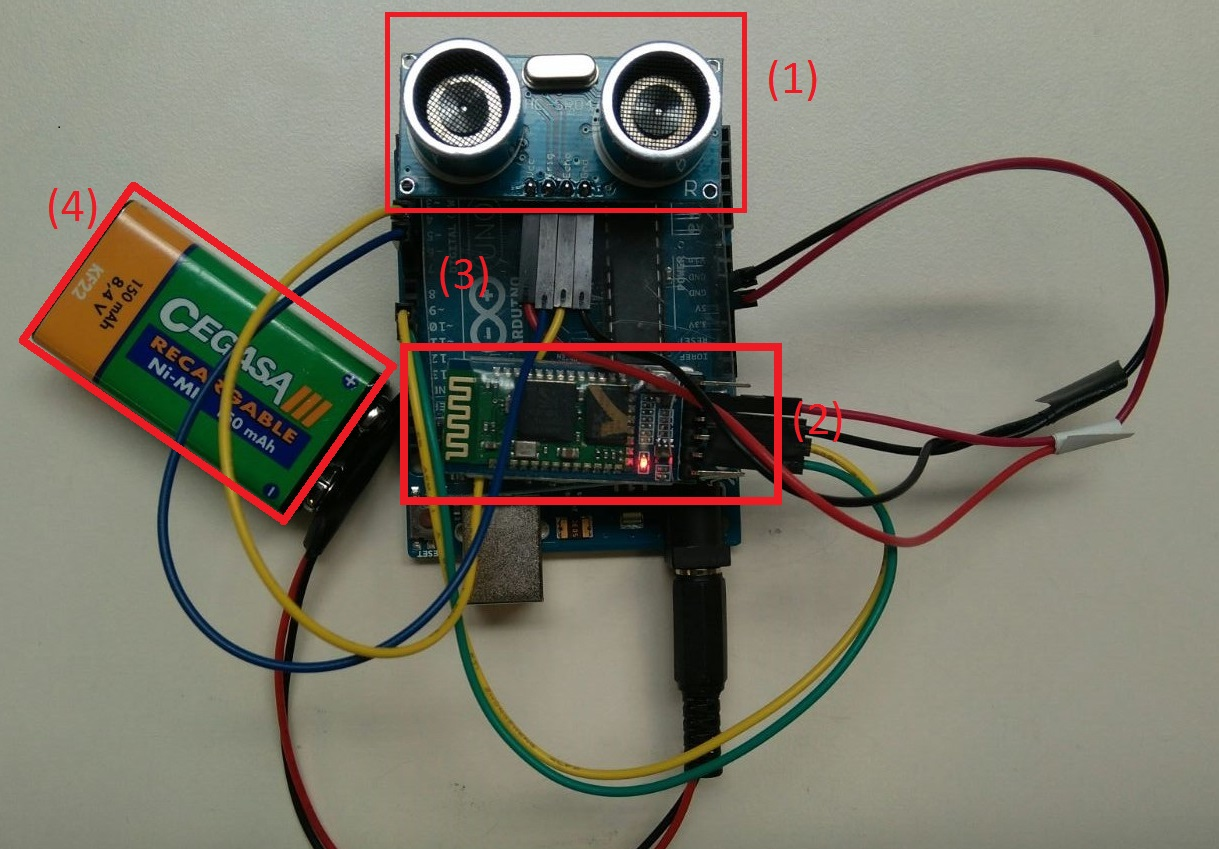
\includegraphics[width=0.7\textwidth]{./graphics/sensor}
 	\caption{Prototipo de sensor de ultrasonidos} \label{fig:sensor_ultrasonido}
 \end{figure}

	\subsubsection{Conexionado del sensor}
		El conexionado del prototipo (apartado \ref{su}), aparece representado de manera esquemática en la Figura \ref{fig:conexionado} con el fin de clarificar las conexiones. En un futuro diseño más compacto, la placa utilizada, así como algunos de los componentes, serán modificados manteniendo el enfoque de bajo coste, ergonomía y precisión. Por ello las conexiones podrán ser modificadas según sea necesario.
		
		 
		\begin{figure}[H]
			\centering
			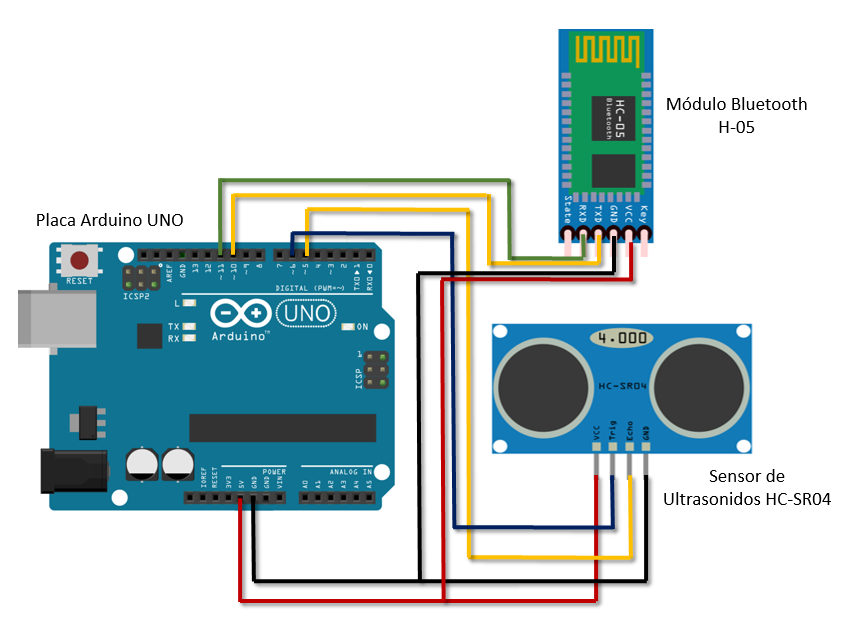
\includegraphics[width=0.7\textwidth]{./graphics/conexionado}
			\caption{Esquema de conexión del sensor de ultrasonido} \label{fig:conexionado}
		\end{figure}
		
	\subsection{Comunicación del sensor}
	
		\subsubsection{Bluetooth}
		
		Para el envío de la información de distancia desde la placa Arduino hasta el PC donde se van a procesar los datos, se ha elegido el módulo comercial Bluetooth H-05 que aparece representado en la Figura \ref{fig:bluetooth}.
		
	
			 \begin{figure}[H]
			 	\centering
			 	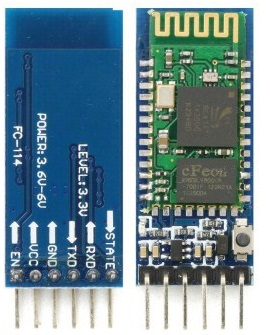
\includegraphics[width=0.25\textwidth]{./graphics/bluetooth}
			 	\caption{Módulo Bluetooth HC-05} \label{fig:bluetooth}
			 \end{figure}
			 
		Dicho módulo se comunicará con un dongle USB 4.0 en el PC ya que éste no dispone de interfaz Bluetooth de serie (ver Figura \ref{fig:dongle}). Además es compatible con estándares anteriores (2.0, 3.0) por lo que resulta apropiado para el diseño.
		
		
		\begin{figure}[H]
			\centering
			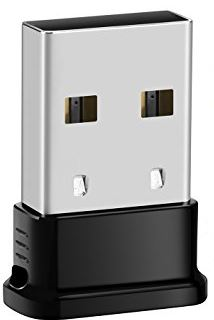
\includegraphics[width=0.15\textwidth]{./graphics/dongle}
			\caption{Dongle Bluetooth 4.0 WhiteLabel} \label{fig:dongle}
		\end{figure}
			
		\subsubsection{Software de captura}
		
		En este trabajo se ha diseñado un software de captura (Figura \ref{fig:software}) para la obtención de los datos de distancia suministrados por el sensor.
		

		Las funcionalidades principales de este software son:
		\begin{enumerate}
				\item Creación del interfaz Bluetooth para la comunicación con Matlab. 
				\item Representación de los datos recogidos en tiempo real.
				\item Posibilidad de guardar los datos en un archivo.
				\item Posibilidad de cargar un archivo y representarlo offline.
		\end{enumerate}
	
		
\section{Procedimiento de medida}		

\subsection{Set-up de medida}
Para demostrar la viabilidad del sistema en cuanto a su capacidad para medir la distancia de separación entre pasos,se proponen dos set-ups que consisten en establecer unas marcas en el suelo a una distancia conocida para así, una vez realizado el procesado de las señales, poder determinar si los resultados son correctos. El primer set-up consta de una medida de paso de 43 cm (ver Figura \ref{fig:setup_43}) y el segundo para una de 80.5 cm (ver Figura  \ref{fig:setup_80} ). 

\begin{figure}[H]
	\centering
	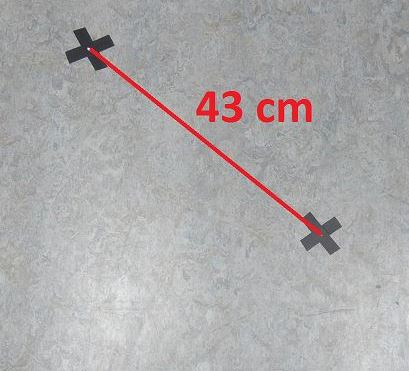
\includegraphics[width=0.55\textwidth]{./graphics/setup_43}
	\caption{Set-up de medida de un paso de 43 cm} \label{fig:setup_43}
\end{figure}

\begin{figure}[H]
		\centering
		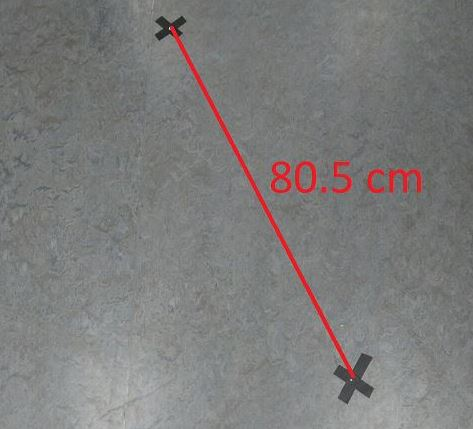
\includegraphics[width=0.55\textwidth]{./graphics/setup_80}
		\caption{Set-up de medida de un paso de 80.5 cm} \label{fig:setup_80}
\end{figure}
	
Este montaje permitirá el poder medir un la distancia de un paso para verificar que el tanto el funcionamiento como el procesado con correctos. Se dejará como línea futura el poder realizar el procesado de forma automática y para varios pasos. Para realizar las medidas se ha colocado un sensor inercial en cada pie y el sensor de ultrasonidos en el tobillo según se representa en la Figura \ref{fig:colocar} y \ref{fig:paso}. 
\begin{figure}[H]
	\centering
	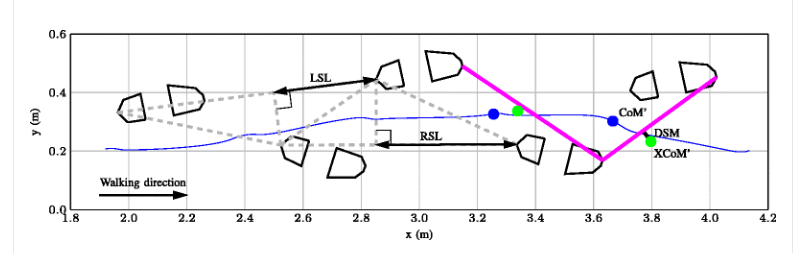
\includegraphics[width=0.55\textwidth]{./graphics/Medida}
	\caption{Colocación de los sensores para la medida} \label{fig:colocar}
\end{figure}
\begin{figure}[H]
	\centering
	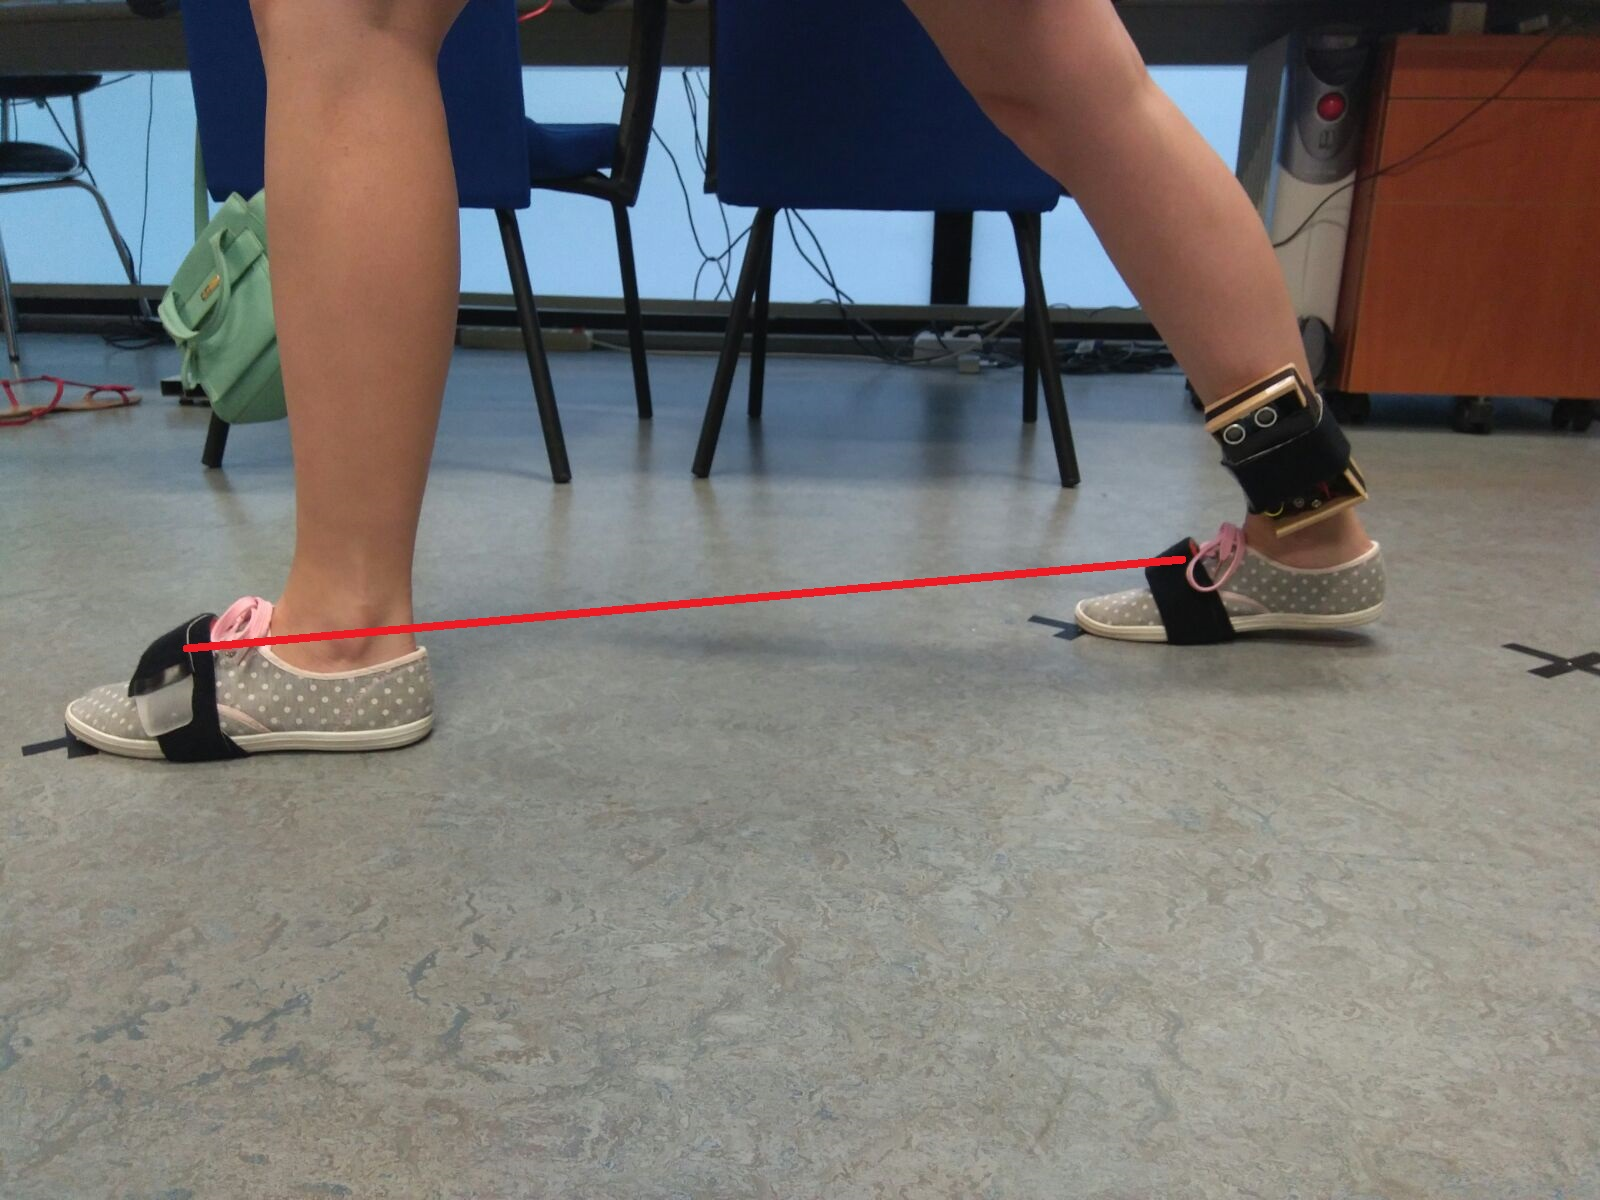
\includegraphics[width=0.65\textwidth]{./graphics/paso}
	\caption{Ejemplo de paso para la medida} \label{fig:paso}
\end{figure}


\subsection{Captura de datos}

Para llevar a cabo la medida se colocará un sensor inercial en cada pie y el sensor de ultrasonidos en uno de ellos. A continuación, se capturarán los datos de los sensores inerciales mediante el software específico MTManager de Xsens y los datos del sensor de ultrasonido mediante el software realizado con MATLAB\textsuperscript{\textregistered} 


\subsection{Sincronización}
Una de las etapas clave del diseño del sistema a tiempo real es el de la sincronización de ambos sensores. En este trabajo, para una demostración de funcionamiento, el procesado de las señales de ambos sensores se realizará por separado de forma que se pueda demostrar el funcionamiento del sistema y se dejará como línea futura de investigación la sincronización. 

Se pretende conseguir una lectura de los datos del sensor de ultrasonido en el PC con un tiempo de muestreo constante. En este punto del trabajo se encuentran dificultades con la forma en que Matlab lee los datos. Los datos enviados por el sensor son constantes pero la lectura hace ese tiempo variable. Si se consigue un tiempo constante, mediante procesados como la interpolación podría sincronizarse con los sensores inerciales. Además, debido a que se utilizan dos programas de captura, es necesario establecer un inicio que se considere como principio tanto para las señales de los sensores inerciales como el de ultrasonidos. 


\subsection{Obtención de distancia}
Para la obtención de la distancia de separación entre pasos existen tres scripts realizados con la herramienta software Matlab\textsuperscript{\textregistered}

Mediante un software en Matlab\textsuperscript{\textregistered} se cargan las señales y se realiza el post-procesado para obtener cada una de las distancias que van a permitir la obtención de la distancia de separación entre pasos.

Se procesará el cálculo de las distancias deseadas de los sensores inerciales y del de ultrasonido y dichas informaciones se utilizarán para la obtención de la distancia de separación entre pasos.

\subsubsection{Sensores inerciales}

	
	Para la obtención del dato de distancia a partir de las señales proporcionados por los sensores inerciales es necesario tener en cuenta que la distancia se recorre en el plano en el que se produce el avance, que es este caso es el plano XY.

Para obtener la posición en este plano a partir de la aceleración en los tres ejes XYZ proporcionada por los sensores inerciales, es necesaria una doble integración.Posteriormente se elimina la deriva existente en las señales debido a esta integración. A continuación se describen los cálculos realizados

\begin{itemize}
	
	\item{\textbf{Obtención de la velocidad}}
	
		Se realiza una primera integración de la aceleración en el eje X y en el eje Y de donde se obtiene la velocidad tal y como aparece en la Figura \ref{fig:vel_no_corr}
	 \begin{figure}[H]
	 	\centering
	 	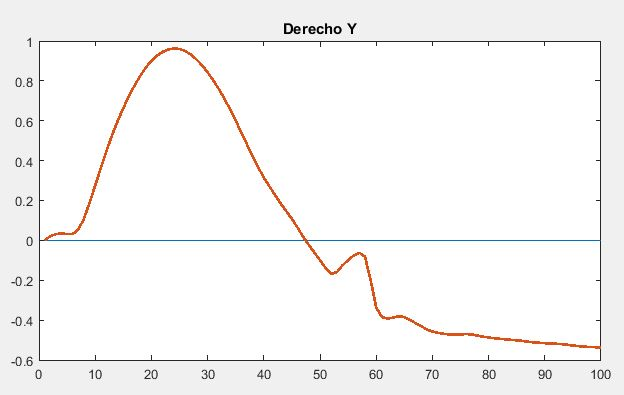
\includegraphics[width=0.81\textwidth]{./graphics/vel_no_corr}
	 	\caption{Ejemplo de deriva en la señal} \label{fig:vel_no_corr}
	 	
	 \end{figure}
 
	\item{\textbf{Obtención de la velocidad sin deriva}}	
	
En el instante de inicio y fin del paso, cuando el pie permanece apoyado, la velocidad debe ser cero.. Para lograr eliminar la deriva en la señal se propone utilizar la ecuación de la recta (color morado) que aparece en la Figura  \ref{fig:vel_no_corr_rect} . Dicha recta entre dos puntos A(a1, a2) y B(b1,b2) se difine mediante la ecuación \ref{eq:recta}
	
	\begin{equation}\label{eq:recta}
	y = (\frac{b_{2}-b_{1}}{a_{2}-a_{1}})*(x-a_{1})+b_{1}
	\end{equation}
	
	;donde:
	\begin{itemize}
		\item b2: coordenada y del último punto escogido (B)
		\item b1: coordenada x del último punto escogido (B)
		\item a2: coordenada x del primer punto escogido (A)
		\item a1: coordenada y del primer punto escogido (A)

	
	\end{itemize}


		 \begin{figure}[H]
		 	\centering
		 	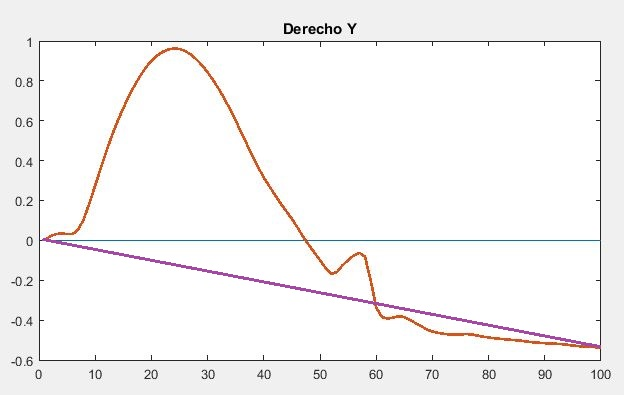
\includegraphics[width=0.8\textwidth]{./graphics/vel_no_corr_deriva}
		 	\caption{Recta para la corrección de la deriva} \label{fig:vel_no_corr_rect}
		 	
		 \end{figure}
De esta forma restando a la señal de velocidad la recta calculada, el resultado es el que aparece en la Figura \ref{fig:corregida} donde se representa la velocidad sin deriva.

	
		 \begin{figure}[H]
		 	\centering
		 	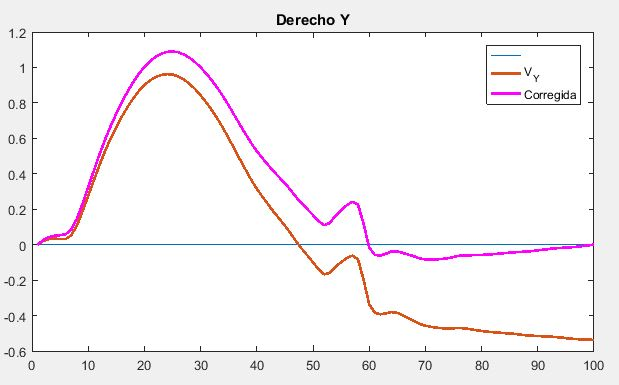
\includegraphics[width=0.8\textwidth]{./graphics/corregida}
		 	\caption{Ejemplo eliminación de la deriva} \label{fig:corregida}
		 \end{figure}


	\item{\textbf{Obtención de distancia D2 de sensores inerciales}}

	
	Una vez corregida la deriva en las velocidades X e Y de los sensores izquierdo y derecho en necesaria una segunda integración para hallar la posición en cada uno de los ejes. A continuación se representa la posición en el eje X con respecto al eje Y para calcular la distancia total en el plano XY (ver Figura \ref{fig:posi})
	\begin{figure}[H]
		\centering
		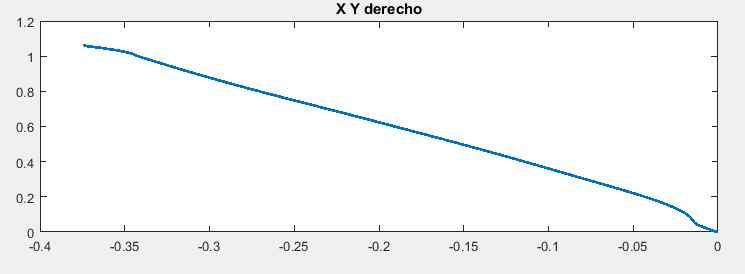
\includegraphics[width=1\textwidth]{./graphics/posi}
		\caption{Ejemplo eliminación de la deriva} \label{fig:posi}
		
	\end{figure}
	
	Para el cálculo de la distancia será necesario la eliminación de la deriva en la posición.
	
	La distancia (D2) ahora será la distancia entre los puntos inicial y final de la Figura \ref{fig:posi}, una vez corregida la deriva, que se calculará mediante la ecuación \ref{eq:pos}
		\begin{equation}\label{eq:pos}
		Distancia = \sqrt{(b_{1}-a_{1})^{2}+(b_{2}-a_{2})^{2}}
		\end{equation}
		\begin{equation}\label{eq:punto2}
			B = [b_{1},b_{2}]	
		\end{equation}
		\begin{equation}\label{eq:puntos1}
			A = [a_{1},a_{2}]
		\end{equation}
		;donde:
		\begin{itemize}
		\item b2: coordenada y del último punto escogido (B)
		\item b1: coordenada x del último punto escogido (B)
		\item a2: coordenada x del primer punto escogido (A)
		\item a1: coordenada y del primer punto escogido (A)
		\end{itemize}
\end{itemize}



\subsubsection{Sensor de ultrasonido}

	Previamente a la obtención de la distancia que se desea obtener usando el sensor de ultrasonido, se realiza una comprobación del correcto funcionamiento tanto del dispositivo como del envío de datos al PC vía Bluetooth. Inicialmente se realizan medidas con el sensor en estático. Para ello se propone el set-up de medida que aparece representado en la Figura  \ref{fig:ultrasonido}.
		
		 \begin{figure}[H]
		 	\centering
		 	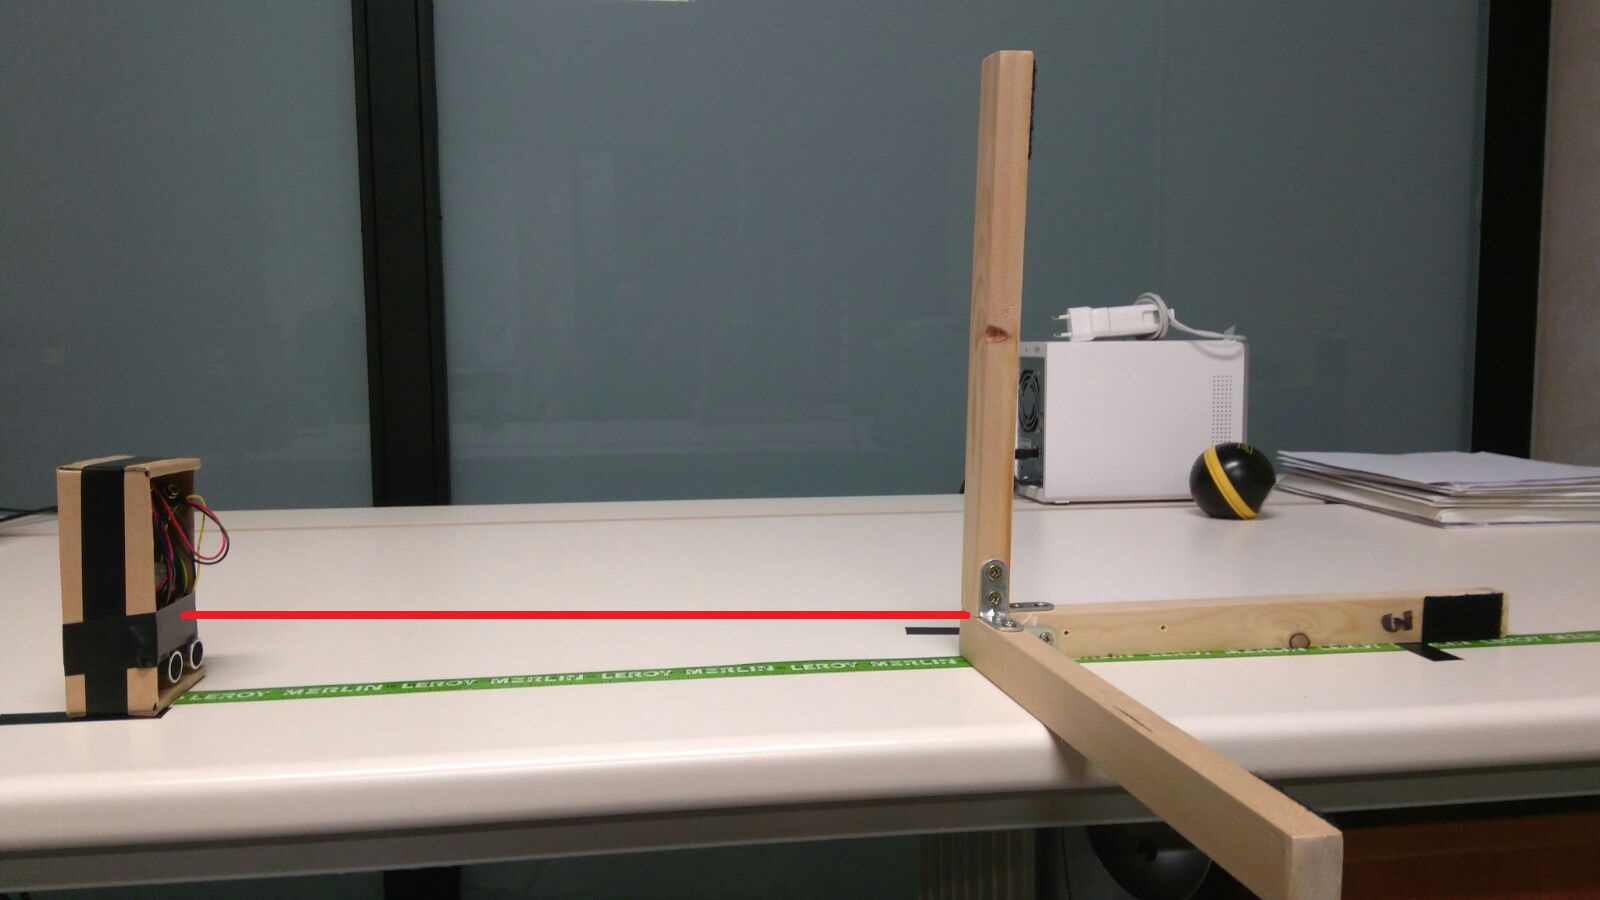
\includegraphics[width=0.95\textwidth]{./graphics/ultrasonido}
		 	\caption{Setup medida estática de sensor de ultrasonido}\label{fig:ultrasonido}
		 \end{figure}

Para estimar la precisión y el correcto funcionamiento del sensor se ha calculado el error absoluto y relativo de cada una de las medidas realizadas.

Una vez hecha dicha comprobación en estático, se añade al sistema de medida completo. Para ello se coloca el sensor en el tobillo y con el sensor orientado hacia la otra pierna (ver Figura \ref{fig:ultracoloc}).
		
	 \begin{figure}[H]
	 	\centering
	 	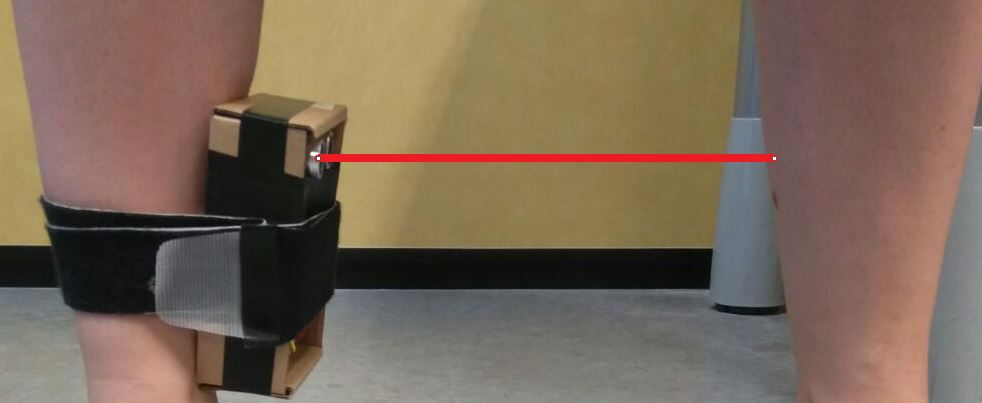
\includegraphics[width=0.8\textwidth]{./graphics/coloc_ultr}
	 	\caption{Colocación de sensor para medidas en dinámico} \label{fig:ultracoloc}
	 \end{figure}
				
		
\subsubsection{Obtención de distancia de separación entre pasos}

Una vez calculadas las distancias necesarias, se procede al cálculo de la distancia de separación entre pasos. En la Figura \ref{fig:sep} se representa dicho cálculo. La distancia D2 es la correspondiente al cálculo de la distancia con el sensor inercial izquierdo en este caso, la distancia D1 es la distancia calculada mediante el sensor de ultrasonido.
\begin{figure}[H]
	\centering
	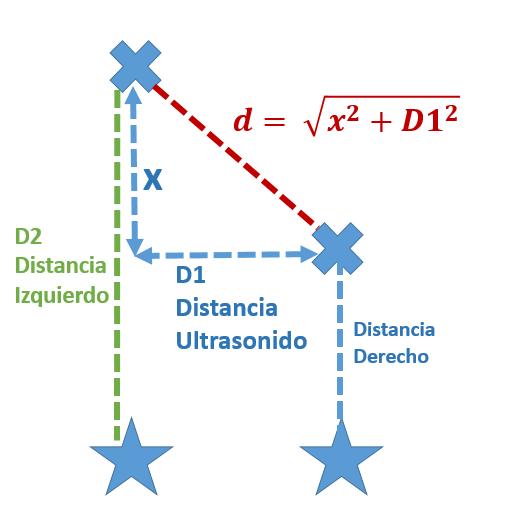
\includegraphics[width=0.8\textwidth]{./graphics/sep}
	\caption{Cálculo final de distancia de separación entre pasos} \label{fig:sep}
\end{figure}

Por tanto, para obtener X se utiliza la ecuación \ref{eq:x}
\begin{equation}\label{eq:x}
x = D2 - DistanciaDerecho
\end{equation}
En el caso de que el primero de los pasos se comenzase con el izquierdo la ecuación es la relativa a la DistanciaIzquierdo.

Para determinar la distancia, se utiliza por tanto, la ecuación \ref{eq:d}
\begin{equation}\label{eq:d}
d = \sqrt{x^{2}+D1^{2}}
\end{equation}
%\thispagestyle{empty}

%
% Solución FBG
%
\chapter{Solución con sensores de fibra FBG\label{sec:FBG}}
%------------------------------
%------___SOLUCIÓN_FBG___------
%------------------------------

\label{sec:FBG3}

\textcolor{rositaoscuro}{
	\textit{
		\colorbox{yellow}{Introducción} breve del guante, que tecnologias implica.
		Resumen fibras de Bragg 
		¿Qué es una fibra FBG?
		¿Porque se utilizan?
		El procesado de las señales resultantes se realiza mediante Labview.
	}
}


 Como primer prototipo se ha estudiado y llevado a cabo un guante cuyo funcionamiento se basa en los sensores de fibra FBG. 
 
 El prototipo consiste en una sección de PDMS con forma de huella de mano que tiene embebida una red en fibra de Bragg. Para la obtención, procesado y visualización de los resultados medidos se emplea el entorno de desarrollo LabVIEW.



%--Marco conceptual
\section{Marco conceptual}
\label{sec:marco3}

Este apartado tiene por finalidad realizar una clara exposición de los conceptos teóricos fundamentales para la comprensión del diseño llevado a cabo. 


%--FIBRA ÓPTICA
\subsection{Fibra óptica}
\label{sec:fibra3}
	\textcolor{rositaoscuro}{
		\textit{
			- -Cómo se propaga la luz en ella.\\
	 		- -Partes de la fibra.\\
			Tipos de emisores (LED Laser).\\
			Receptores.\\
			Conectores y soldaduras.\\
			- -Fabricación.\\
			- -Tipos de fibra.\\
		}
	}

	%-- ¿Qué es la fibra óptica y la comunicación óptica?
	La fibra óptica es una hebra de material dieléctrico, así cómo el vidrio (sílice) o el polímero acrílico. 
	Se emplea como medio de propagación de señales luminosas. Es decir, para transmitir ondas electromagnéticas del espectro óptico: regiones espectrales de infrarrojo, luz visible y ultravioleta. En la siguiente imagen (figura \ref{fig:espectroOptico}) se puede observar dentro del espectro electromagnético dónde se sitúa el espectro óptico.	 
	
	\begin{figure}[H]
		\centering
		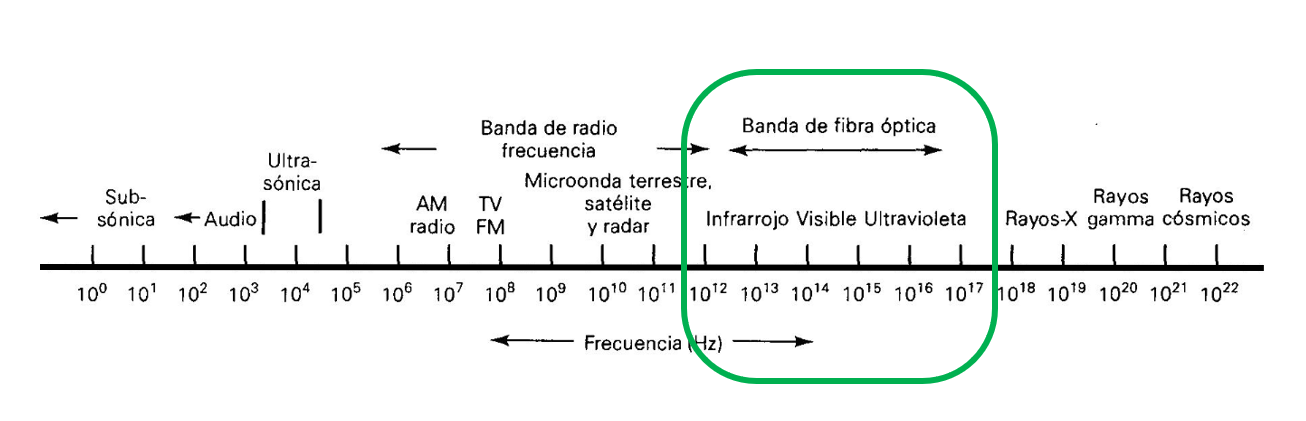
\includegraphics[width=0.95\textwidth]{./img/espectrooptico}
		\caption{Espectro electromagnético en frecuencia.}
		\label{fig:espectroOptico}
	\end{figure}
	
	%--Ventanas de comunicación por FO
	Cabe destacar que dentro del espectro óptico las longitudes de onda habituales para comunicación en fibra óptica están entre los 700nm y 1600nm. Estas se dividen en rangos con mejores características para la transmisión, denominadas ventanas de comunicación. Como se muestra en la figura \ref{fig:ventanaOptica}, son tres las ventanas más utilizadas,\cite{ventanasFO}:
 	\begin{table}[H]
		%\centering
		\hspace{2cm}
		\renewcommand{\arraystretch}{2}
		\begin{tabular}{rrl}
			\textbf{1ª ventana}& 800 a  900 nm  & $\longmapsto$ $\,$ longitud de onda utilizada = 850nm  \\
			\textbf{2ª ventana}& 1250 a 1350 nm & $\longmapsto$ $\,$ longitud de onda utilizada = 1310nm  \\
			\textbf{3ª ventana}& 1500 a 1600 nm & $\longmapsto$ $\,$ longitud de onda utilizada = 1550nm   \\ 
		\end{tabular} 
	\end{table}

	 \begin{figure}[H]
	 	\centering
	 	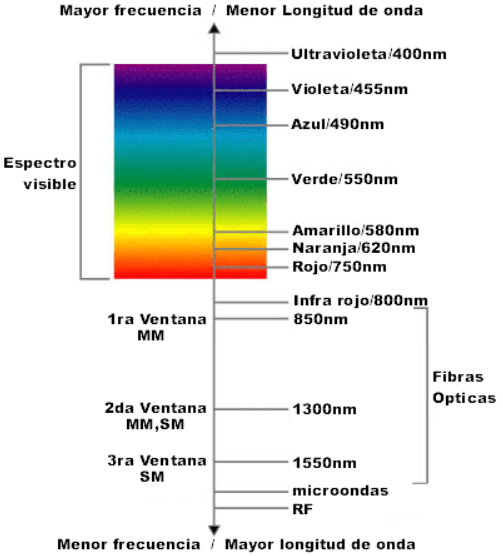
\includegraphics[width=0.5\textwidth]{./img/ventana}
	 	\caption{Longitud de onda fibra óptica junto con el espectro visible. \cite{ventanasFO}}
	 	\label{fig:ventanaOptica}
	 \end{figure}
 	La razón de que las ventanas de comunicación utilizadas se sitúen en las frecuencias indicadas reside en los diferentes comportamientos que tiene la atenuación de las señales en función de la longitud de onda (ver figura \ref{fig:perdidasFrec}). Existen algunas zonas dónde la atenuación es mínima, coincidiendo con la segunda y la tercera ventana. En cambio, en la zona correspondiente a la primera ventana las pérdidas no son mínimas, pero sí que se mantienen constantes. 	
 	
 	\begin{figure}[H]
 		\centering
 		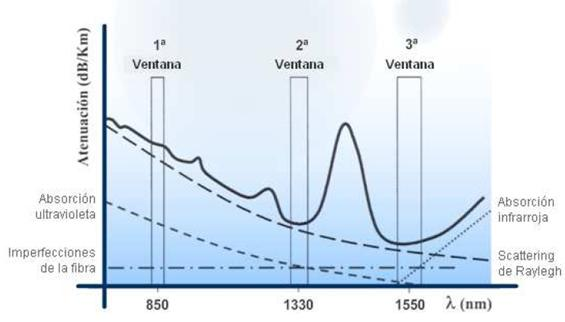
\includegraphics[width=0.8\textwidth]{./img/perdidasFrec}
 		\caption{Atenuación(dB/Km) frente a longitud de onda  $\lambda$ (nm) \cite{imgRadioModo}}
 		\label{fig:perdidasFrec}
 	\end{figure}

 %-- Características físicas de la fibra
 En cuanto a las propiedades físicas de la fibra óptica, son bastante delicadas ya que su grosor no supera por mucho al diámetro del cabello humano y se obtiene de la extrusión del sílice, SiO\textsubscript{2} , es decir, se trata de un filamento de vidrio muy fino. Es por ello que es la fibra óptica estándar está rodeada de una cubierta protectora. 
 
  \begin{figure}[H]
  	\centering
  	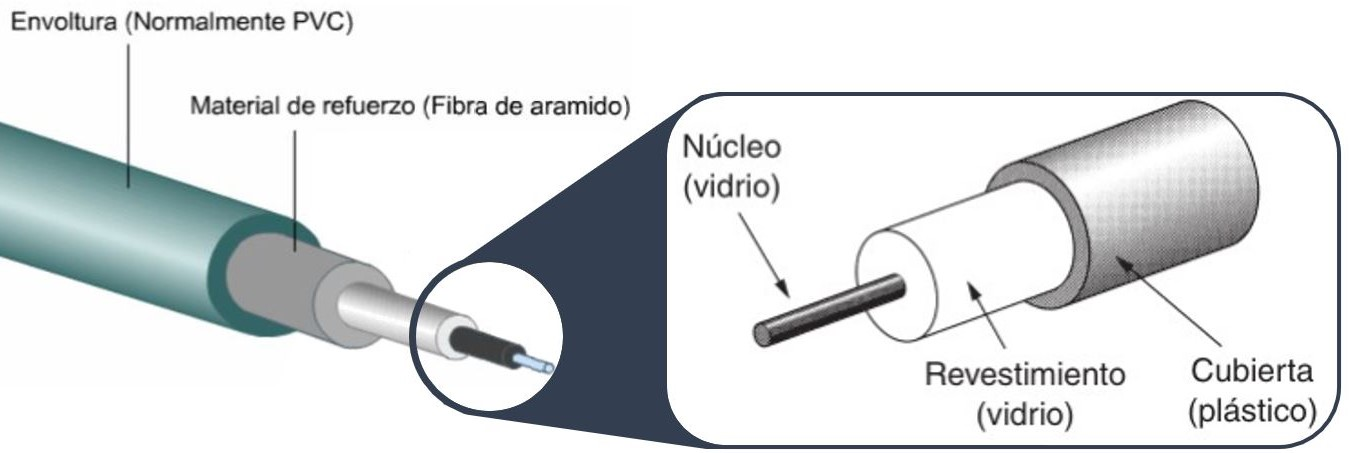
\includegraphics[width=0.87\textwidth]{./img/capas-fibra2}
  	\caption{Capas fibra óptica \cite{imgNucleoFibra,imgCapasFO}} 
  	\label{fig:capasFibra}
  \end{figure} 
  
  
  
 La fibra óptica estándar cuenta varias capas (figura \ref{fig:capasFibra}): núcleo, revestimiento y cubierta (o buffer).  Si la aplicación lo permite, conviene proteger la fibra con más capas externas. En la imagen anterior la fibra está además protegida por un material de refuerzo (fibra de aramido) y una envoltura (PVC).
 
 Tanto el núcleo cómo el revestimiento forman el medio por el cual se propaga la luz. Estas dos capas son tan finas que forman un filamento flexible, pero muy delicado, puesto que es muy propenso a romperse ante dobleces u otras manipulaciones externas. Por ello el resto de las capas son tambien importantes por proporcionar a la fibra protección y haciendo posible su utilización es escenarios de despliegue.
 
 %-- Fabricación FO
 La fabricación de la fibra óptica es un proceso de alta tecnología. Es importante mantener la pureza y la regularidad del núcleo. Esto es complejo, puesto que estamos hablando en algunos casos de núcleos de un grosor entorno a las 8 micras (en fibras monomodo). El grosor estándar de la fibra es de 125 micras(una micra equivale a una millonésima parte de un metro). Para conseguir este resultado el proceso de fabricación consiste en reproducir a escala macroscópica la estructura de la fibra que se quiere obtener. Esta reproducción a gran escala de la fibra deseada se le denomina preforma. Una vez se tiene la preforma, esta se va fundiendo y estirando hasta alcanzar el filamento del diámetro deseado. De una preforma se pueden sacar kilómetros de fibra. Para fabricar la preforma se parte de una barra de vidrio hueca (el vidrio que formará el recubrimiento) y se baña en un gas que contiene unas partículas (lo que formará el núcleo). Al calentar a mil grados, las partículas comienzan a fundirse hasta que el tubo colapsa y forma una vara maciza, que es la preforma. Para fundirla y estirarla esta se coloca verticalmente y se calienta. La complejidad de esta fase reside en mantener constante el flujo y el diámetro del hilo resultante. Además durante esta fase se aprovecha para crear una capa protectora sobre el vidrio (cubierta en la figura \ref{fig:capasFibra}). Finalmente los kilómetros de fibra óptica se enrollan en grandes bobinas. \cite{fabricacionFO}
 
 %-- Fibra Monomodo y multimodo
  \begin{figure}[H]
 	\centering
 	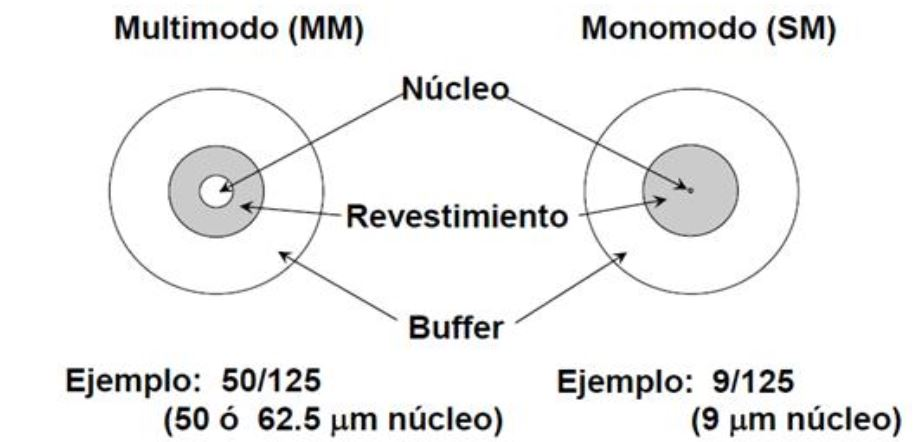
\includegraphics[width=0.6\textwidth]{./img/MM-SM}
 	\caption{Relación grosor fibra multimodo (MM) y monomodo (SM) \cite{imgRadioModo} } 
 	\label{fig:modoMonoMulti}
 \end{figure} 
 
  Dependiendo de la relación de diámetro entre el núcleo y el revestimiento, la fibra fibra será monomodo o multimodo (figura \ref{fig:modoMonoMulti}). Esta diferencia afecta a la propagación de la luz dentro de la guía de onda (figuras \ref{fig:guiaMM}, \ref{fig:guiaSM}, \ref{fig:indiceMultimodo}). Ya se ha comentado que el diámetro de la fibra es de aproximadamente 125 micras. En el caso de las fibras monomodo, el núcleo de estas tiene un diámetro tan pequeño (en torno a 8 micras) que la luz solo puede propagarse en un sólo modo (rayo). Sin embargo, en el caso de las fibras multimodo, al poseer un núcleo mayor (entre 50 o 62.5 micras) soportan la transmisión el múltiples modos, es decir, los rayos de luz viajan en muchas direcciones a través de este. \cite{FOA} 
   
   	\begin{figure}[H]
		\centering
		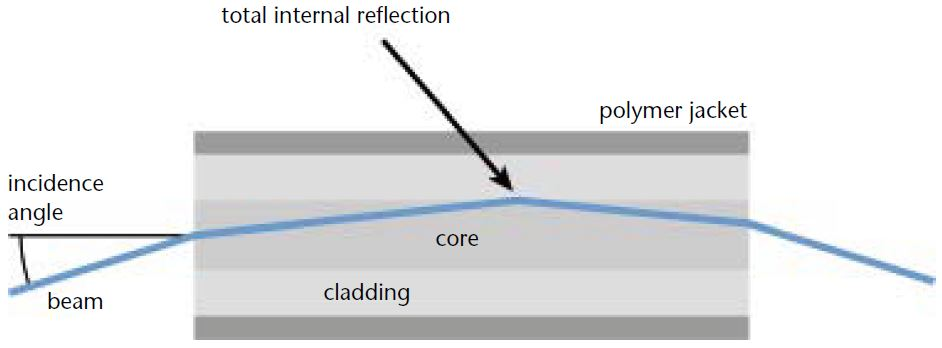
\includegraphics[width=0.7\textwidth]{./img/guiaMM}
		\caption{Corte transversal fibra multimodo en transmisión de luz. \cite{imgMonoMulti} } 
		\label{fig:guiaMM}
	\end{figure} 
  	\begin{figure}[H]
		\centering
		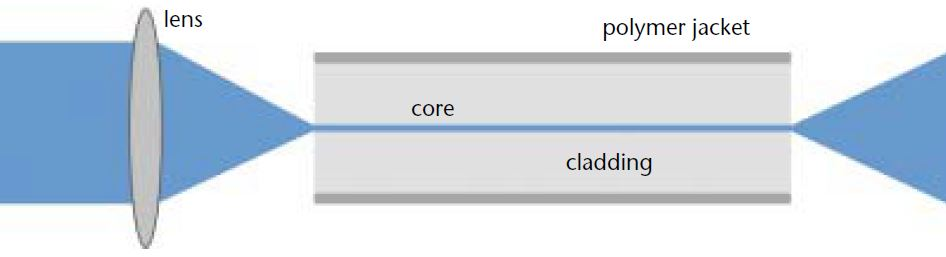
\includegraphics[width=0.7\textwidth]{./img/guiaSM}
		\caption{Corte transversal fibra monomodo en transmisión de luz. \cite{imgMonoMulti} } 
		\label{fig:guiaSM}
	\end{figure}  
 	
 	%-- Relación monomodo y multimodo con las longitudes de onda
 	Relacionando los tipos de fibras ópticas con las ventanas en las que trabajan, las fibras multimodo suelen trabajar en primera y segunda ventana, mientras que las fibras monomodo en segunda y tercera. 

	  	\begin{figure}[H]
		\centering
		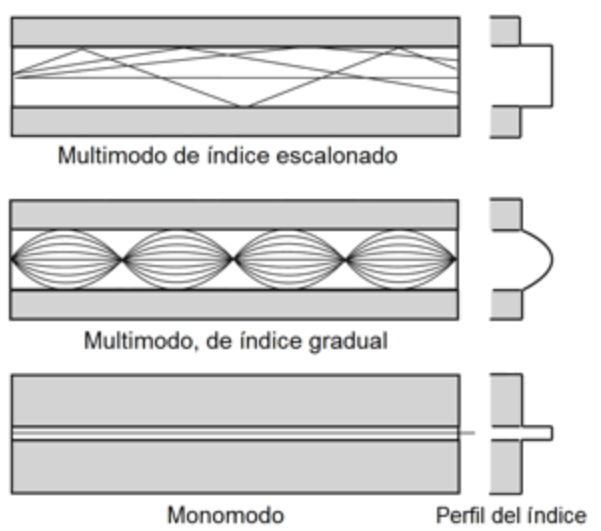
\includegraphics[width=0.5\textwidth]{./img/transFO-esc-grad}
		\caption{Disposición rayos. Multimodo (indice escalonado y gradual) y monomodo. \cite{FOA} } 
		\label{fig:indiceMultimodo}
		\end{figure}
	
 	%-- Otros tipos de FO
 	Además existen otros tipos de fibras menos comunes: la fibra de plástico (POF) y la fibra de sílice con revestimiento de plástico (HCS/PCS). La primera tiene un núcleo de gran diámetro ($1mm$ aproximadamente), puede utilizarse para redes de distancia corta y de baja velocidad. Las fibras de sílice con revestimiento de plástico tienen un núcleo más pequeño ($200\mu m$ aproximadamente) que las fibras de plástico. Estos dos últimos tipos de fibra multimodo generalmente son de índice escalonado, mientras que el resto de fibras multimodo suelen ser de índice gradual. En la figura \ref{fig:indiceMultimodo} se observa como es la diferencia en la distribución de los rayos en un caso y en el otro. En cuanto al tamaño de las fibras, la figura \ref{fig:otrosTiposFO} se representan las diferentes relaciones de tamaños entre los cinco tipos de fibra vistos. \cite{FOA}
 	 	
 	 \begin{figure}[H]
 	 	\centering
 	 	
\includegraphics[width=0.7\textwidth]{./img/tiposFO}
 	 	\caption{Relación tamaños fibras ópticas. \cite{FOA} } 
 	 	\label{fig:otrosTiposFO}
 	 \end{figure} 	
  	
 %-- PROPAGACIÓN DE LA LUZ	
 %-- Diferenci de indices de refracción
 La diferencia de índices de refracción entre las capas centrales de la fibra son las que permiten la propagación de la luz a través de esta. El núcleo tiene un mayor indice de refracción que el revestimiento, lo que genera que los rayos de luz se curven a medida que pasan del núcleo al revestimiento, generando una "reflexión interna total" en la fibra. La siguiente imagen (figura \ref{fig:TIR}) sirve para explicar claramente este concepto:
 
 \begin{figure}[H]
 	\centering
 	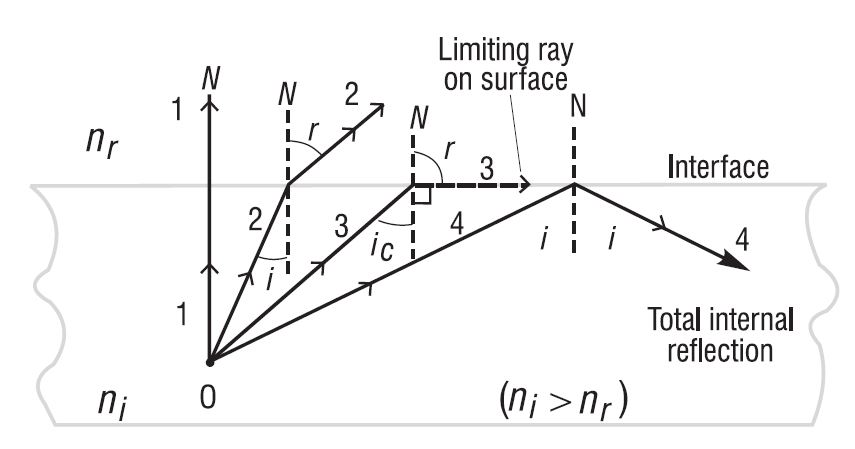
\includegraphics[width=0.66\textwidth]{./img/TIR}
 	\caption{Ángulo crítico y reflexión interna total. \cite{geometriaBasicaFP} } 
 	\label{fig:TIR}
 \end{figure}
 
 %Reflexión interna total
 En la figura \ref{fig:TIR} se ilustran cuatro rayos que se originan en el puno 0, lo que sería el núcleo de la fibra óptica (dónde el indice de refracción \textit{n\textsubscript{i}} es mayor). Entre los cuatro rayos varía el ángulo con el que estos inciden sobre el revestimiento (de menor índice de refracción\textit{n\textsubscript{r}}). Se observa cómo en el rayo número 1 incide con $90\,^{\circ}$ (incidencia normal), no habiendo reflexión y siguiendo el rayo en la misma dirección. En el rayo número 2 incide con un ángulo \textit{i}, y se refracta con \textit{r}. El rayo número 3 incide con el ángulo crítico \textit{i\textsubscript{c}}, suficientemente grande para que el rayo reflejado se propague a lo largo de la interfaz entre los dos medios, quedando atrapado. Por último, el rayo número 4 incide con un ángulo \textit{i} superior al ángulo crítico (ecuación \ref{eq:angCritico}), \textit{i\textsubscript{c}}, consiguiendo que se refleje totalmente en el mismo medio del que incide. Este rayo obedece a la ley de reflexión, siendo su ángulo de reflexión exactamente igual a su ángulo de incidencia. Este fenómeno se denomina \textit{"Reflexión interna total"}, necesario para que suceda la transmisión de señales lumínicas en la fibra óptica. 

	\begin{equation}
		\label{eq:angCritico}
		\hat{i}\textsubscript{c} =  \sin^{-1}\left(\dfrac{n\textsubscript{r}}{n\textsubscript{i}}\right)
	\end{equation}

 La reflexión interna total atrapa la luz hasta cierto ángulo en el núcleo, definiendo la apertura numérica a la que hay que asegurarse de penetrar la luz para que se de el fenómeno de reflexión interna total. Así se fuerza a que la mayoría de los rayos de luz incidan sobre el interfaz y se reflejen, permitiendo la transmisión de la señal lumínica. 
 
 
 \textcolor{rositaoscuro}{//----------------------------------------------------------------------- }\\ 
 %No vamos a hablar más de multimodo
 \textcolor{teal}{(\\Puesto que en la solución llevada a cabo en este trabajo se utilizan fibras monomodo no se va a extender el texto en explicar más conceptos sobre la transmisión en fibras multimodo.\\)\\
 \textcolor{rositaoscuro}{-------------------------------------------------------------------------//}\\}
 
 
 %Sistemas de propagación
   \begin{figure}[H]
 	\centering
 	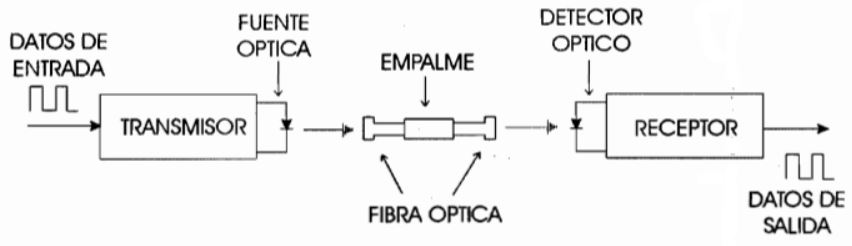
\includegraphics[width=1\textwidth]{./img/TxFOp2p}
 	\caption{Transmisión punto a punto de señales a través de fibra óptica. \cite{txFO} } 
 	\label{fig:TxFOp2p}
 \end{figure} 
 
 Los sistemas de propagación de señales luminosas a través de la fibra óptica componen un medio de transmisión de datos rápido y fiable. En la figura \ref{fig:TxFOp2p} se plasma el procedimiento que sigue la transmisión de datos en un sistema óptico y los elementos que lo componen. Previa a la propagación a través de un medio óptico de una señal eléctrica (analógica o digital) es necesario realizar una conversión de esta a señal óptica. Esto genera una señal óptica a partir de una señal eléctrica en el emisor o fuente de luz situado en el extremo inicial de la comunicación. Realizada la conversión, la señal es transmitida a lo largo de la fibra óptica. Según las características del escenario puede haber una o varias uniones entre fibras a lo largo del canal. Estás pueden realizarse empalmando o utilizando conectores. Una vez la señal óptica atraviesa todo el canal, llega al detector, dónde sucede el proceso inverso al ocurrido en el emisor y a la salida del sistema completo se tiene la señal eléctrica. Esta corresponde a la señal introducida al sistema con una pequeña posibilidad de haber sufrido pérdidas o atenuación debido a la impureza de la fibra, la distancia, las conexiones entre elementos del sistema o cualquier otro evento ajeno al este. Estas modificaciones de la señal de entrada pueden ser contrarrestadas o solventadas en recepción sin suponer un impedimento a una comunicación exitosa.    
  
 Veamos por separado los elementos dibujados en la figura \ref{fig:TxFOp2p}:
 	\begin{itemize}
 	%-Emisores (Transmisión)
 		\item \textit{\textbf{Emisores (Transmisión)}}	
 		% \hspace{0.2cm} 
 		Los emisores de luz forman un papel imprescindible en la transmisión de señales a través de la fibra óptica. Se encargan de convertir la señal eléctrica a señal luminosa, para que esta se pueda propagar por el canal óptico según lo esperado. Principalmente hay dos tipos de fuentes de luz: diodos LED o diodos láser. Dentro de los de tipo láser se distinguen otros tres tipos: láser fabry-perot (\textit{FP}), láser de retroalimentación distribuida (\textit{(DFB)}) y láser de cavidad vertical y emisión superficial (\textit{VCSEL}). Unas de las condiciones más importantes que deben cumplir las fuentes de luz son que operen en la longitud de onda adecuada, se puedan de modular lo suficientemente rápido para transmitir datos y poder acoplarse de forma eficiente a la fibra. \cite{TransRecepFO}
 		
 		 \begin{figure}[H]
 			\centering
 			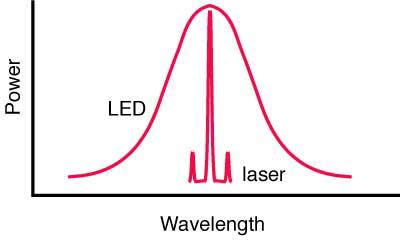
\includegraphics[width=0.35\textwidth]{./img/led-laser}
 			\caption{Relación entre potencia y longitud de onda diodo LED frente a diodo láser. \cite{FOA} } 
 			\label{fig:ledVsLaser}
 		\end{figure} 
 	 	\begin{figure}[H]
 			\centering
 			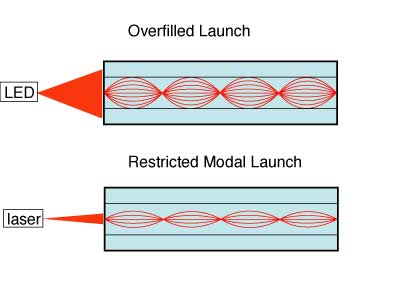
\includegraphics[width=0.55\textwidth]{./img/led-laserEMISION}
 			\caption{Corte transversal de fibra con emisión desde diodo LED frente a diodo láser. \cite{FOA} } 
 			\label{fig:corteledVsLaser}
 		\end{figure} 
 		
 		\begin{itemize}
 			\item \textbf{LED} - \textit{Light Emitting Diodes}\\
 			Consiste en una fuente de luz incoherente. Es una fuente de luz de mayor ancho de banda de operación que en el caso de los diodos láser (véase figura \ref{fig:ledVsLaser} y \ref{fig:corteledVsLaser}). Tiene un espectro de emisión entre los 30-100 nm. En función del material semiconductor con el que se fabrique se pueden emitir desde luz ultravioleta hasta infrarrojos. Para conseguir emitir en un espectro reducido, es necesario polarizarlo y hacerle circular corriente eléctrica. Pueden ser modulados sin dificultad hasta velocidades de 100-200 Mb/s y en algunos casos hasta velocidades de 1 Gb/s. 
 			
 			Además, tienen un comportamiento simple, de fácil fabricación y tienen un coste bajo en comparación a otras fuentes. Su circuitería de alimentación y control es muy sencilla, debido a los bajos niveles de corriente que son necesarios para que funcione el dispositivo y a su relativa inmunidad frente a variaciones de la temperatura. Necesitan baja potencia de alimentación. Su geometría y patrón de radiación es de alta divergencia, el acoplo de luz a la fibra óptica monomodo es difícil, especialmente en los LED de emisión superficial. Son dispositivos fiables, ya que no sufren la degradación de tipo catastrófico y son menos sensibles que los diodos láser a la degradación por envejecimiento. \\
 			
 					\textcolor{rositaoscuro}{//-Resumen: Los LED se basan en emisión espontánea. Por sus características (baja coherencia, divergencia alta, baja potencia óptica de salida, circuitos electrónicos sencillos,...) se emplean habitualmente en combinación con fibras multimodo para enlaces de distancias cortas y velocidades bajas.}
 			
 			\item \textbf{Láser} - \textit{Light Amplification by Stimulated Emission of Radiation}\\
 			Consiste en un tipo de fuente de luz coherente. Tienen mayor capacidad de transmisión de luz, concentran la luz en forma de haces estrechos pero potentes, es decir, emiten de manera direccional e intensa. Es por ello que se suele advertir que mirar con los ojos directamente a este tipo de emisiones es peligroso para la vista. (Véanse figuras \ref{fig:ledVsLaser} y \ref{fig:corteledVsLaser}). Pueden ser modulados en frecuencia y a gran velocidad. Su geometría y patrón de radiación es de relativamente baja divergencia, el acoplo de luz a la fibra óptica monomodo es bastante eficiente. Su composición es más compleja que la del diodo LED. Para conseguir dicha directividad y potencia, internamente la fuente tiene cavidades que combinan medio activo y espejos. Por ejemplo, necesita tener un circuito de realimentación para su control, debido a que se ve afectado por las variaciones de temperaturay a las reflexiones que pueda provocar la potencia óptica incidente en su salida. Debido a ello, son complejos y costosos de fabricar. 
 			
 					\textcolor{rositaoscuro}{//- Resumen Los láseres se basan en emisión estimulada, conseguida formando cavidades que combinan medio activo y espejos para la realimentación. Son de mayores prestaciones que los LED (mayor coherencia, más directivos, mayor potencia de salida,...), pero más complejos y caros. Se pueden usar en fibras monomodo. Los hay de dos tipos, básicamente:\\
 					--Láseres multimodo (Fabry-Perot) que se usan en enlaces de velocidades medias/bajas para distancias medias/cortas\\
 					-- Láseres monomodo (DFB,DBR) que se usan en enlaces de alta capacidad –alta velocidad, distancias largas- y en sistemas WDM}
 			
 			
 		\end{itemize}
  		
  		La tabla \ref{tabla:caractFuentes} compara las características de las diferentes fuentes mencionadas, permitiendo ver también las diferencias entre los diferentes tipos de diodos láser citados.
  		
  		
  		\begin{table}[H]
  			\begin{tabular}{l|c|c|c|c|}
  				\cline{2-5}
  				& \cellcolor[HTML]{EFEFEF}\textbf{LED} & \cellcolor[HTML]{EFEFEF}\textbf{LD F-P} & \cellcolor[HTML]{EFEFEF}\textbf{LD\_DFB} & \cellcolor[HTML]{EFEFEF}\textbf{VCSEL} \\ \hline
  				\multicolumn{1}{|l|}{\cellcolor[HTML]{EFEFEF}Espectro emisión}                 & Ancho                                & Medio                                   & \multicolumn{2}{c|}{Estrecho}                                                     \\ \hline
  				\multicolumn{1}{|l|}{\cellcolor[HTML]{EFEFEF}Directividad}                     & Muy divergente                       & \multicolumn{3}{c|}{Directivo}                                                                                              \\ \hline
  				\multicolumn{1}{|l|}{\cellcolor[HTML]{EFEFEF}Potencia}                         & Baja                                 & \multicolumn{3}{c|}{Alta}                                                                                                   \\ \hline
  				\multicolumn{1}{|l|}{\cellcolor[HTML]{EFEFEF}Velocidad / BW modulación}        & Varios cientos de MHz                & \multicolumn{3}{c|}{Varias decenas de GHz}                                                                                  \\ \hline
  				\multicolumn{1}{|l|}{\cellcolor[HTML]{EFEFEF}Acoplo a la fibra}                & MMF                                  & \multicolumn{2}{c|}{SMF}                                                           & MMF                                    \\ \hline
  				\multicolumn{1}{|l|}{\cellcolor[HTML]{EFEFEF}Curva I-P}                        & Sin $I_{umbral}$; baja pendiente          & \multicolumn{3}{c|}{Con $I_{umbral}$; alta pendiente}                                                                            \\ \hline
  				\multicolumn{1}{|l|}{\cellcolor[HTML]{EFEFEF}Dependencia con temperatura}      & Baja                                 & \multicolumn{3}{c|}{Alta}                                                                                                   \\ \hline
  				\multicolumn{1}{|l|}{\cellcolor[HTML]{EFEFEF}Circuitos electrónicos asociados} & Sencillos                            & \multicolumn{3}{c|}{Complejos}                                                                                              \\ \hline
  				\multicolumn{1}{|l|}{\cellcolor[HTML]{EFEFEF}Seguridad para la vista}          & No peligroso                         & \multicolumn{3}{c|}{Potencialmente dañino}                                                                                  \\ \hline
  				\multicolumn{1}{|l|}{\cellcolor[HTML]{EFEFEF}Tiempo vida útil}                 & Alto                                 & \multicolumn{3}{c|}{Medio (suficiente)}                                                                                     \\ \hline
  				\multicolumn{1}{|l|}{\cellcolor[HTML]{EFEFEF}Coste}                            & Bajo                                 & Medio                                   & Alto                                     & Bajo                                   \\ \hline
  				\multicolumn{1}{|l|}{\cellcolor[HTML]{EFEFEF}Ventana operación}                & 1ª, 2ª                               & \multicolumn{2}{c|}{2ª, 3ª}                                                        & 1ª, 2ª                                 \\ \hline
  			\end{tabular}
  		\caption{Tabla características fuentes de ópticas}
  		\label{tabla:caractFuentes}
  		\end{table}
  	
   	%-Detectores (Recepción)		
 		\item \textit{\textbf{Detectores (Recepción)}}
 			
 		En cuanto al proceso de recepción, consiste en que la señal llega al final del canal y se tiene que dar el proceso inverso que en transmisión. Los detectores tienen la función de convertir las señales ópticas a señales eléctricas para recuperar la información. Son diodos semiconductores encargados de polarizar inversamente la polarización realizada en el diodo emisor.  Al igual que pasaba en la transmisión, existe detección coherente o incoherente(detección directa). El componente del receptor que realiza la conversión óptico-eléctrica es el fotodetector. Se distinguen varios tipos, los más comunes son: los fotodidos PIN y los fotodiodos de efecto de avalancha (\textit{APD}). Aunque merece la pena mencionar los fotoespectrómetros, formados por células CCD integradas y una estructurá optica tan precisa que es capaz de detectar la potencia que la luz recibida proporciona en cada longitud de onda. Volviendo a los receptores PIN y APD, además del fotodetector, el detector puede estar compuesto por un pre-amplificador óptico, pero casi siempre tendrá un pre-amplificador eléctrico para amplificar la señal eléctrica obtenida del fotodiodo, de muy baja corriente. El receptor lo podrá formar también (figura \ref{fig:diagRX}) un filtro óptico, para tomar solo en cuenta las frecuencias de interés. Posterior a la pre-amplificación eléctrica, los elementos de procesado de la señal que se incluyan dependerán del si las señales empleadas por el sistema eléctrico son analógicas o digitales.
 		
	 	\begin{figure}[H]
	 		\centering
	 		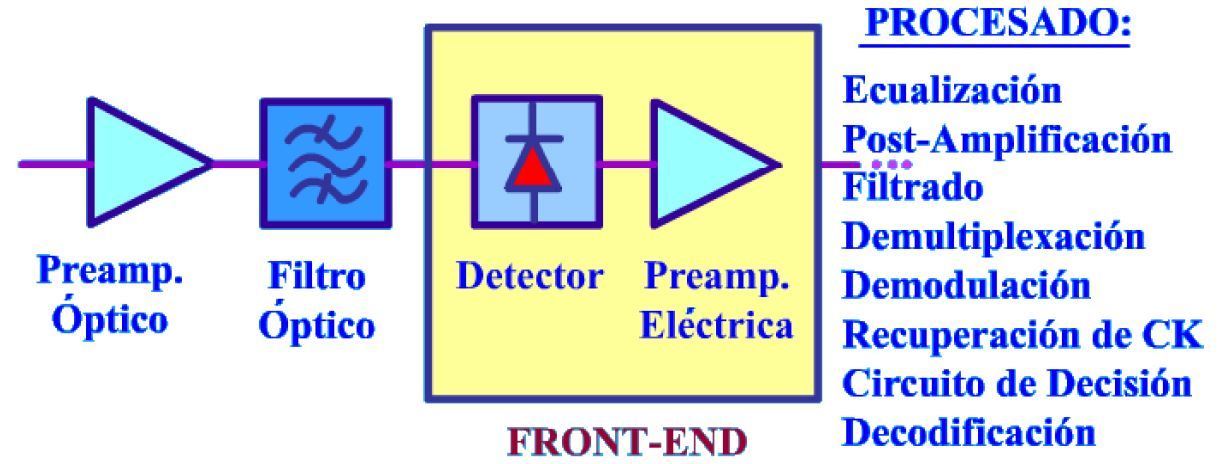
\includegraphics[width=0.65\textwidth]{./img/diagRX}
	 		\caption{Diagrama de bloque receptor} 
	 		\label{fig:diagRX}
	 	\end{figure} 
 	
 		Idealmente los fotodetectores deberián ser altamente sensibles, con alta velocidad de respuesta, poco ruidosos, compactos, robustos y de respuesta lineal. En la práctica es complicado conseguir todos estos atributos en conjunto. Por ejemplo, los APD requieren menor potencia óptica para funcionar que los diodos PIN, pero cuatro veces mayor voltaje de alimentación.
 		
 		\textcolor{rositaoscuro}{//---------------------------------------------------Puedo añadir si eso lo que pone en el siguiente link:}
 		\url{http://www.thefoa.org/tech/ref/appln/transceiver.html}
 	
 	%-Conectores y empalmes
 		\item \textit{\textbf{Conectores y empalmes}}\\

 		Cabe hablar también de los conectores ópticos y empalmes utilizados para unir fibra óptica a fibra óptica u otros elementos del sistema. Teniendo una fibra óptica terminada en algún tipo de conector esta se puede unir a elementos como emisores, receptores, multiplexores y otros elementos, incluso se puede unir a otra fibra terminada en conector con un adaptador macho a macho. Además, para unir dos trozos de fibra es posible realizar una fusión que empalme ambas terminaciones de la fibra. La principal diferencia entre estos dos tipos de uniones es que los conectores unen de manera no permanente, mientras que los empalmes son uniones permanentes. 
 		
 		\begin{figure}[H]
 			\centering
 			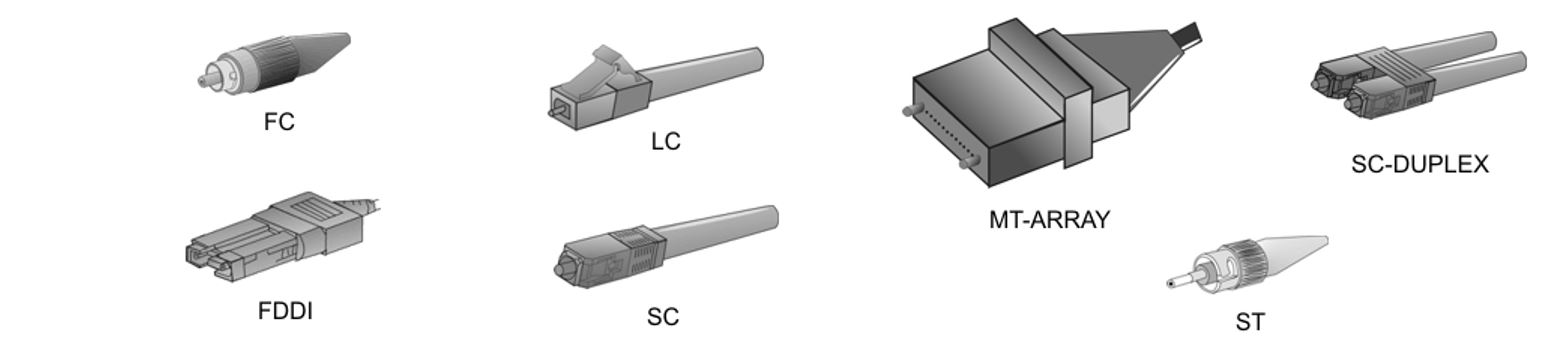
\includegraphics[width=0.95\textwidth]{./img/tiposConect2}
 			\caption{Tipos de conectores de fibra óptica. \cite{TipConectoresFO}} 
 			\label{fig:tiposConect}
 		\end{figure} 
 		
 		Es importante que las uniones no afecten a la calidad de la transmisión, es decir, deben garantizar bajas pérdidas de conectividad. En la figura \ref{fig:tiposConect} se muestra algunos de los conectores más empleados, cada uno de ellos suelen utilizarse en diferentes aplicaciones según sus características. Por ejemplo los utilizados en este trabajo, los conectores FC (\textit{Ferule Connector}) se suelen utiliza tanto en montaje de laboratorio como de campo y sirven en fibras monomodo y multimodo. Además tienen unas pérdidas de inserción IL < 0.34 dB en fibras multimodo y IL < 0.15 dB en fibras monomodo. \cite{TipConectoresFO}\\
 		\begin{figure}[H]
	 		\centering
	 		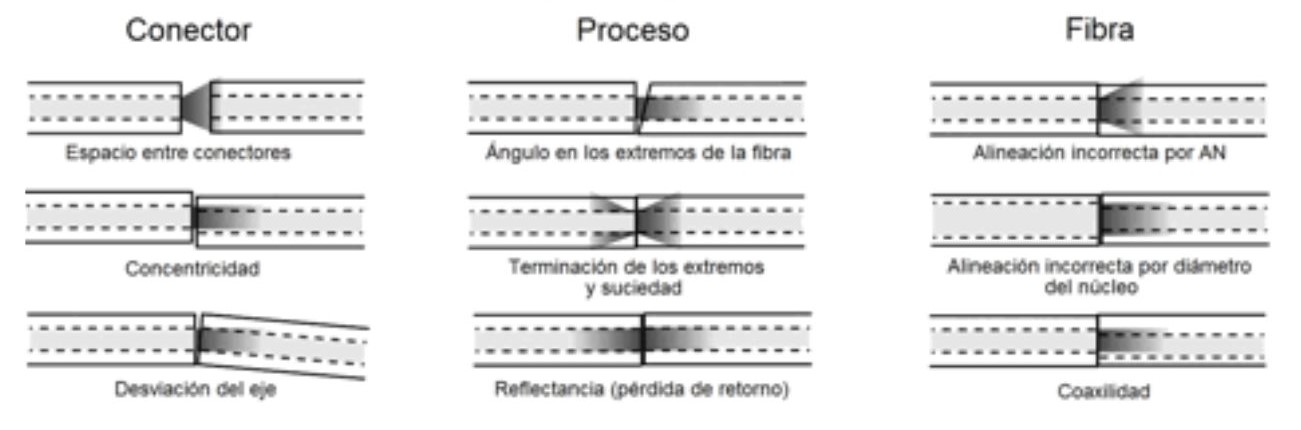
\includegraphics[width=0.85\textwidth]{./img/perdidasOpticas}
	 		\caption{Causas de pérdida óptica en las uniones. \cite{FOAconect}} 
	 		\label{fig:conectLoss}
 		\end{figure}
 		Las pérdidas se pueden reducir cuando los núcleos de las dos fibras son idénticos, están alineados de manera perfecta y se tocan entre sí, los conectores y los empalmes se realizaron adecuadamente y no hay suciedad en la unión. En la figura \ref{fig:conectLoss} se pueden observar diferentes causas de pérdidas en las conexiones de fibra óptica. Además, los conectores pueden tener diferentes formas de férulas (o terminaciones), diferentes tipos de pulidos en el extremo de la fibra donde se realiza la unión (figura \ref{fig:tiposPulidos}), lo que afecta también a las pérdidas resultantes. El extermo de la fibra tiene que estar debidamente limpio y pulido para reducir al máximo ñas pérdidas, ya que una superficie aspera puede dispersar o absorber luz.		
   		\begin{figure}[H]
   			\centering
   			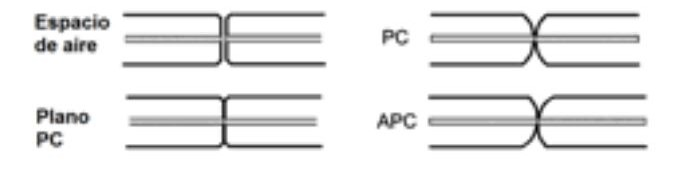
\includegraphics[width=0.55\textwidth]{./img/conectoresPulido}
   			\caption{Tipos de conectores según su pulido. \cite{TipConectoresFO}} 
   			\label{fig:tiposPulidos}
   		\end{figure}

 		En cuanto a los empalmes, que crean una unión permanente entre dos fibras, hay dos tipos: por fusión y mecánicos. En la figura \ref{fig:empalmeTipo} se observa en primer lugar un empalme por fusión y los demás son mecánicos. Los más realizados son los empalmes por fusión por la fiabilidad y la robustez de la unión, así como por brindar pérdidas y reflectancias menores.
 		
 		\begin{figure}[H]
 			\centering
 			\includegraphics[width=0.5\textwidth]{./img/tiposEmpalme}
 			\caption{Tipos de empalmes. \cite{FOAconect}} 
 			\label{fig:empalmeTipo}
 		\end{figure} 
 	
 		 
 		
 		El proceso de fusión (Figura \ref{fig:procFusion}) consiste en primero pelar, limpiar y cortar los extremos de las fibras que se desee unir. Una vez se dispone en los extremos de la fibra desnuda, cortada con la cortadora de precisión y limpia con un paño adecuado y alcohol, se deben colocar cada una en las guías de la fusionadora. Después se ejecuta el programa de fusión adecuado, según sea la fibra. Por último, se le coloca a la fusión un manguito protector termocontraible o una protección tipo mordaza para que la fusión no se desprenda ante alguna adversidad.
 		
 		\begin{figure}[H]
 			\centering
 			\includegraphics[width=0.85\textwidth]{./img/procesoFusion}
 			\caption{Proceso de empalme por fusión. \cite{FOAconect}} 
 			\label{fig:procFusion}
 		\end{figure}

 	 \end{itemize}					

%-- SENSORES ÓPTICOS	
\subsection{Sensores ópticos} %Tipos de sensores ópticos
\label{sec:sensores3}

		
		Existen en el mercado diversos tipos de sensores ópticos. Estos se pueden clasificar atendiendo a diversos aspectos. A continuación se exponen dos clasificaciones básicas\cite{sensoresOpticos}: 

			\begin{itemize}
				\item[$\cdot$] \underline{En función de la naturaleza del parámetro a cuantificar}
				\begin{itemize}
					\item Sensores químicos: Sirven para detectar variación de cantidad de ciertos componentes químicos. Además en este grupo se incluyen los biosensores.
					\item Sensores físicos: Utilizados para medir parámetros físicos (temperatura, presión, espesor, etc.)
				\end{itemize}
				\item[$\cdot$] \underline{En función de la naturaleza de la propiedad óptica medida}
				\begin{itemize}
					\item Sensores de absorbancia
					\item Sensores de reflectancia
					\item Sensores se luminiscencia (fluorescencia, quimioluminiscencia y bioluminiscencia)
					\item Sensores de dispersión Raman
					\item Sensores de índice de refracción
					\item etc.
				\end{itemize}
				\end{itemize}
			
			
				En este trabajo se van a utilizar sensores de difracción de Bragg, que son sensores que cuantifican parámetros físicos a través de mediciones ópticas del índice de refracción.
		
	\begin{itemize}
		\item \textit{\textbf{Redes de difracción de Bragg \textit{(FBG - Fiber Bragg Grating)}}}	
		
		\begin{figure}[H]
			\centering
			\includegraphics[width=0.85\textwidth]{./img/operacionFBG}
			\caption{Funcionamiento de un sensor de fibra óptica FBG \cite{funcionamientoFBG}} 
			\label{fig:funcionamientoFBG}
		\end{figure}		
		
		Los sensores de fibra óptica basados en redes de difracción de Bragg (\textit{Fibre Brag Gratings}), también denominadas FBGs, están diseñados para reflejar longitudes de onda determinadas (según el diseño) de la luz y transmitir el resto (Figura \ref{fig:funcionamientoFBG}). Para ello se crea en el núcleo de la fibra una variación periódica del índice de refracción, conocido cómo rejilla tipo Bragg. Esta variación sólo afecta a la transmisión de cierta longitud de onda, la que refleja. Este tipo de fenómeno se puede utilizar cómo filtro bloqueador de una longitud de onda, además de para medir parámetros físicos cómo la deformación o la temperatura. Por ejemplo, es muy común su uso para la monitorización de estructuras como puentes \cite{FOSensorFrancis}. 
		
		\begin{figure}[H]
			\centering
			\includegraphics[width=0.75\textwidth]{./img/FBGmanufactur}
			\caption{Proceso de generación del sensor de Bragg en la fibra. \cite{tesisUPMmalte}} 
			\label{fig:manufacturaBragg}
		\end{figure}
		
		 Para conseguir en el núcleo la variación permanente del índice de refracción se utiliza una fuente de luz ultravioleta (UV). De esta manera se inscribe una rejilla tipo Bragg en una fibra monomodo (figura \ref{fig:manufacturaBragg}). Comúnmente se utiliza fibra de sílice dopada con germanio, por su fotosensibilidad (capacidad de cambio del índice de refracción del núcleo con la exposición a la luz UV). En función de la intensidad y la duración de la exposición y de la fotosensibilidad de la fibra se consigue una variación del índice de refracción mayor o menor. 
		
		En resumen, los sensores de fibra de Bragg consisten en una fibra óptica monomodo, dónde, en un segmento reducido de esta, se encuentra una rejilla tipo Bragg. Siendo esta la que genera en el núcleo de la fibra el cambio periódico de índice de refracción \cite{defFBG}.\\
		
		Existe una relación matemática entre la longitud característica de la FBG o longitud de la onda reflejada ($\lambda\textsubscript{B}$), el índice de refracción efectivo ($\eta\textsubscript{eff}$) y el periodo de la red de Bragg ($\Lambda$), como se puede ver en la ecuación \ref{eq:condicBragg}, dónde se define la longittud de la onda reflejada, $\lambda\textsubscript{B}$: 
			\begin{equation}
				\label{eq:condicBragg}
				\lambda=\lambda\textsubscript{B} = 2\eta\textsubscript{eff}\Lambda	
			\end{equation}
				
		A partir de estos conocimientos se deduce cómo funciona la medición de deformaciones. Cuando se genera una deformación de la fibra y cambia la distancia entre las rejillas de Bragg, se genera una variación del índice de refracción al variar el periodo de la red de Bragg. Es decir, al deformarse la FBG se tiene una $\Lambda$ diferente respecto a la de reposo, cuando no se genera ninguna deformación. En el caso de las variaciones de temperatura generan un cambio de índice de refracción del silicio, debido al efecto termoóptico \cite{termoDeformFBG}. 
		
		\begin{figure}[H]
			\centering
			\includegraphics[width=0.85\textwidth]{./img/medicBragg}
			\caption{Representación esquemática de un sistema de  medición de deformaciones mediante fibras ópticas con redes de Bragg y analizador espectral óptico. \cite{tesisUPMmalte}} 
			\label{fig:medicBragg}
		\end{figure}
		
		Para utilizar las FBGs cómo sensores se puede construir una distribución como la de la figura \ref{fig:medicBragg}. En primer lugar, se manda un pulso a través de la fibra, y se pone un analizador de espectros para anotar las variaciones en la longitud de onda de Bragg ($\lambda\textsubscript{B}$). Según sea el escenario a sensar pueden ser necesarias más de una FBG. Para ello se puede realizar una configuración en serie (empalmando FBGs) o en paralelo (utilizando multiplexores). 
		
		\begin{figure}[H]
			\centering
			\includegraphics[width=0.65\textwidth]{./img/flexibleFBG}
			\caption{FBG embebida en un material flexible. \cite{nedomaPDMS}} 
			\label{fig:flexibleFBG}
		\end{figure}
	
		Además, para proteger la FBG es conveniente cubrirla con un material flexible (figura \ref{fig:flexibleFBG}), como por ejemplo el policloruro de vinilo (PVC) o el polidimetilsiloxano (PDMS). En este trabajo se utiliza como material protector y estructura del guante el PDMS, expuetso en el siguiente punto.
	
\end{itemize}


%-- POLIDIMETILSILOXANO - PDMS	
\subsection{Polidimetilsiloxano (\textit{PDMS})}
\label{sec:pdms3}
	
	Dentro de la familia de los polímeros orgánicos basados en silicio se encuentra el polidimetilsiloxano, también conocido como PDMS. Otro término por el que se le conoce es dimeticona, un tipo de aceite de silicona. Para abreviar, a partir de este punto en el documento se referirá a él como PDMS. El polidimetilsiloxano es un material cristalino, flexible y fácil de modelar \cite{propPDMS}.
	
	\begin{figure}[H]
		\centering
		\includegraphics[width=0.45\textwidth]{./img/compPDMS}
		\caption{Composición química del PDMS. \cite{nedomaPDMS}} 
		\label{fig:compFBG}
	\end{figure}
	
	Su formulación química es $(H_{3}C)_{3}SiO[Si(CH_{3})_{2}O]_{n}Si(CH_{3})_{3}$ (figura \ref{fig:compFBG}), siendo $[Si(CH_{3})_{2}O]_{n}$ el monómero presente n veces en la molécula del PDMS según la proporción de este con el agente de curación \cite{propPDMS}.  	
 
 	Para su fabricación se mezcla el monómero con el agente de curación siguiendo una proporción n:1, en función de la consistencia con la que se desee el elastómero resultante. Cuanto mayor sea la n, mayor será la solidez del PDMS. Una vez hecha la mezcla es necesario que esta cure, ya sea a temperatura ambiente o aplicándole calor para que cure más rápidamente.
  
 	\begin{figure}[H]
	 	\centering
	 	\includegraphics[width=0.49\textwidth]{./img/liquidoPDMS}
	 	\includegraphics[width=0.49\textwidth]{./img/solidoPDMS} 
	 	\\(a)\hspace{7cm}(b)
	 	\caption{(a) PDMS en estado líquido \cite{liquidoPDMS} (b) PDMS en estado sólido, trás la curación \cite{solidoPDMS}} 
	 	\label{fig:slPDSM}
	 \end{figure}
  \textcolor{teal}{TENGO QUE ELEGIR ENTRE UNA PAREJA DE IMAGENES U OTRA, O UNA DE CADA. Debajo dejo los links de las de abajo por si necesito ponerlos en la bibliografia.\\}
  	\begin{figure}[H]
	 	\centering
	 	\includegraphics[width=0.49\textwidth]{./img/liquidPDMS}
	 	\includegraphics[width=0.49\textwidth]{./img/solidPDMS} 
	 	\\(a)\hspace{7cm}(b)
	 	\caption{(a) PDMS en estado líquido \cite{liquidoPDMS} (b) PDMS en estado sólido, trás la curación \cite{solidoPDMS}} 
	 	\label{fig:slPDSM2}
	 \end{figure}
 
 	\url{https://www.elveflow.com/microfluidic-tutorials/soft-lithography-reviews-and-tutorials/introduction-in-soft-lithography/pdms-softlithography-replication/}
 
	\url{https://www.instructables.com/id/Making-a-PDMS-Microfluidic-Device-With-Maskless-Mo/}
	
  	 La utilización de este elastómero en el ámbito de este trabajo es una buena opción ya que es inofensivo, no tóxico, no inflamable y eléctricamente no conductor.\cite{nedomaPDMS}

	% Material empleado para embeber las FBGs.


		
%-- LABVIEW 	
\subsection{LabVIEW (\textit{\underline{Lab}oratory \underline{V}irtual \underline{I}nstrument \underline{E}ngineering \underline{W}orkbech})}

\label{sec:labview3}



	\begin{figure}[H]
		\centering
		\includegraphics[width=0.45\textwidth]{./img/LabVIEWicon}
		\caption{Logo LabVIEW. }
		\label{fig:LabVIEWicon}
	\end{figure}

	LabVIEW es un software de National Instruments de ingeniería que pretende simplificar el diseño de sistemas software distribuidos de pruebas, medidas y control \cite{LabVIEWpage}. Es un lenguaje y un entorno de programación gráfica desarrollado por National Instruments. 
	
	En sus inicios LabVIEW estaba orientado únicamente a aplicaciones de control de equipos electrónicos utilizados para el desarrollo de sistemas de instrumentación. Tiene dos ventanas principales: el \textbf{Panel frontal} y el \textbf{Diagrama de bloques}, como se ve en la figura \ref{fig:ejLabVIEW}. El panel frontal alberga los botones, pantallas, etc. con el que el usuario interactúa una vez está desarrollado el software, interfaz de usuario. Mientras que el diagrama de bloques corresponde a la circuitería interna del programa, dónde se interconectan los elementos del panel frontal para operar con ellos, dando lugar a la programación del backend del software \cite{LabVIEWbook}. 
	
  	\begin{figure}[H]
		\centering
		\includegraphics[width=0.95\textwidth]{./img/LabVIEWej}
		\\\hspace{2.5cm}(a)\hspace{6.5cm}(b)
		\caption{(Ejemplo sencillo de LabVIEW: (a) Frontend; (b) Backend}\cite{LabVIEWyt} 
		\label{fig:ejLabVIEW}
	\end{figure}

	En LabVIEW la programación se realiza en el Diagrama de bloques. Los programas están compuestos por los siguientes elementos: controles, funciones e indicadores. Estos elementos se conectan mediante ``cables''. De esta manera se genera el programa, definiendo la ``circulación'' de los datos.  
	

 \textcolor{rositaoscuro}{asdf}
 \textcolor{teal}{sdffsd}
%--Desarrollo del prototipo



\section{Desarrollo del prototipo}
\label{sec:prototipo3}
%[Esta parte de desarrollo del proyecto parte de otro trabajo. Aquí mencionar algo que diga el trabajo de Silvia y mencionarla en la bibliografía.]

La realización del primer desarrollo se origina a partir de un trabajo realizado con anterioridad en el grupo de investigación de la universidad\cite{SilviaTFM}. Se mejora el soporte físico (hardware) y se desarrolla un nuevo programa con un interfaz de usuario simple e intuitivo.
El prototipo consiste en un prototipo técnico y funcional de un guante sensorizado para medir los ángulos de flexión de los nudillos y la muñeca.

 \textcolor{rositaoscuro}{Tengo que sacar una foto mejor que esta donde se vean además el interrogador y la fuente.!!!}
	\begin{figure}[H]
		\centering
		\includegraphics[width=0.85\textwidth]{./img/prototipo}
		\caption{Prototipo con Sensores de fibra FBG.} \label{fig:prototipoFBG}
	\end{figure}


 
\subsection{Materiales}
\label{sec:materiales3}
En este apartado se disponen brevemente los componentes utilizados para el desarrollo del prototipo. 

\begin{figure}[H]
	\centering
	\includegraphics[width=0.60\textwidth]{./img/fibraBraggpaquete2}
	\caption{FBG de longitud de onda de 1536nm en su envoltura de compra.} \label{fig:FBGpaquete}
\end{figure}

Las fibras de rejilla de Bragg (FBG) empleadas son de la empresa Micron Optics (ver figura \ref{fig:FBGpaquete}). Consisten en un FBG centrado en una óptica recubierta don poliimida de dos metros de longitud. Se emplean las siguientes longitudes de onda para cada FBG según la flexión a medir:

\begin{table}[H]
	\centering
	\begin{tabular}[t]{|r|c|}
		\hline
		& Longitud de onda del sensor\\
		\hline
		\hline
		Dedo pulgar & 1532 nm \\
		\hline
		Dedo índice & 1548 nm \\
		\hline
		Dedo corazón & 1576 nm \\
		\hline
		Dedo anular & 1568 nm \\
		\hline
		Dedo meñique & 1560 nm \\
		\hline
		Muñeca & 1541.26 nm \\
		\hline
	\end{tabular}
	\caption{Tabla longitud de cada sensor FBG}
	\label{tabla:mmedidas 80 cm}
\end{table}

Puesto que las fibras de Bragg resultan muy sensibles ante roturas y la aplicación del prototipo precisamente consiste en contorsionar las fibras es necesario embeber las fibras en un material moldeable pero rígido. Para ello se emplea PMDS, cuyas características ya se citan con anterioridad en este documento. En los siguientes apartados se expone con más detalle la fabricación del guante en PDMS. 

El conexionado entre el guante y los demás elementos que componen el prototipo se realiza con cables de fibra óptica monomodo unidos a través de conectores o empalmes. Los empalmes se han realizado mediante fusión con protección termocontraible. Los conectores utilizados para la fibra son los de Férula (\textit{Ferule Connector - FC}).

Para que llegue el pulso transmitido a cada una de las fibras de Bragg hace falta un dispositivo que se capaz de dejar pasar la luz de una sola fibra a varias y combinar en el sentido inverso los pulsos de luz que retornen. Esta función la cumple un divisor de fibra óptica. Se ha empleado un splitter de PLC de una entrada y ocho salidas terminadas en conectores de férula, de las cuales sólo serán necesarias seis (ver figura \ref{fig:splitter}).

\begin{figure}[H]
	\centering
	\includegraphics[width=0.75\textwidth]{./img/splitter1a8}
	\caption{Splitter de PLC de 1:8} \label{fig:splitter}
\end{figure}

En cuanto a la transmisión de la luz y su posterior recepción se necesita una fuente y un interrogador. 

La fuente es un emisor de luz de banda ancha que puede provenir de un diodo superluminiscente (SLED) o de emisión espontánea amplificada (ASE).  La fuente integrada en el prototipo es la fuente de diodo superluminiscente (SLED) DL-BP1-1501A de Ibsen Photonics (ver figura \ref{fig:FuenteInterrogador}). Esta fuente es comunmente utilizada para sistemas que utilizan FBGs. Emite pulsos de 70nm de ancho de banda en el rango de los 1550nm. La versión empleada dispone de una interfaz de LabView que permite configurar sus parámetros de emisión cuando fuera necesario. La fuente necesita ser configurada una vez y funciona según su última configuración la próxima vez que se encienda. 

El interrogador es el dispositivo que detecta la señal de luz proveniente de la fibra y, en este escenario, la transmite al ordenador. En este proyecto se trabaja con el interrogador USB I–MON 256/512 del proveedor Ibsen Photonics, al igual que la fuente (ver figura \ref{fig:FuenteInterrogador}). Este interrogador incluye un software implementado en LabView que sirve de herramienta para el usuario para visualizar la detección de luz desde el ordenador a través del puerto USB en tiempo real.  Este software sirve de base para la realización del interfaz de este proyecto. 

\begin{figure}[H]
	\centering
	\includegraphics[width=0.49\textwidth]{./img/fuente}
	\includegraphics[width=0.49\textwidth]{./img/interrogador} 
	\\(a)\hspace{7cm}(b)
	\caption{(a) Fuente \cite{fuente} (b) Interrogador \cite{interrogador}} 
	\label{fig:FuenteInterrogador}
\end{figure}



Para el desarrollo del software se utiliza un portátil Asus GL502VSK con 32,0 GB de memoria física (RAM) y un procesador Intel(R) Core(TM) i7-7700HQ CPU @ 2.80GHz.  

Además se han diseñado y fabricado el molde para fabricar el molde y  un armazón para almacenar de manera organizada y segura el cableado de las fibras junto con el splitter.

\subsection{Instrumental}
\label{sec:instrumental3}
Este prototipo conlleva el uso de una variada instrumentación. A continuación se mencionan algunos de los instrumentos físicos más notables empleados.  

Para la manufacturación del molde y del armazón se ha empleado tecnología de impresión 3D en material plástico PLA. Se han utilizado dos modelos de impresora debido a la disponibilidad de estas en la universidad, la impresora Hephestos de BQ y Witwox de BQ también (ver figura \ref{fig:impresoras3D}). Son muchos los materiales con los que se pueden realizar impresiones en 3D a partir de un diseño, en este caso se ha escogido el PLA por ser barato y suficiente para las características necesarias en el prototipo.
    
\begin{figure}[H]
	\centering
	\includegraphics[width=0.49\textwidth]{./img/hephestos}
	\includegraphics[width=0.49\textwidth]{./img/witbox} 
	\\(a)\hspace{7cm}(b)
	\caption{(a) Hephestos (b) Witbox} 
	\label{fig:impresoras3D}
\end{figure}

Para la fabricación del guante de PDMS se han empleado herramientas que ha simple vista pueden parecer de aplicación tan dispares como una báscula, un horno y una empalmadora de fibra (ver figura \ref{fig:herramientas}; \ref{fig:empalmadora}). La báscula utilizada es la disponible en el laboratorio de la universidad tiene ua precisión de miligramos y en este proyecto se utiliza para utilizar con exactitud la proporción del monómero y el agente de cura en la disolución de PDMS. El horno se emplea para conseguir que el PDMS se cure con la ayuda del calor en menos tiempo.

\begin{figure}[H]
	\centering
	\includegraphics[width=0.3\textwidth]{./img/bascula}
	\includegraphics[width=0.3\textwidth]{./img/horno} 
	\\(a)\hspace{4cm}(b)
	\caption{(a) Báscula (b) Horno } 
	\label{fig:herramientas}
\end{figure}

Para empalmar los sensores de FBG con el resto del prototipo se emplea una empalmadora de fibra. La empalmadora utilizada tiene la ventaja de incluir un apartado para fundir los protectores termocontraibles de empalmes. 

\begin{figure}[H]
	\centering
	\includegraphics[width=0.3\textwidth]{./img/empalmadora}
	\caption{Empalmadora de fibra} \label{fig:empalmadora}
\end{figure}


\subsection{Proceso de fabricación del soporte físico}
\label{sec:proceso3}
%Elaboración

 \textcolor{rositaoscuro}{Elaboración/Proceso de fabricación}

Para que sea más cómoda la explicación del proceso de elaboración del prototipo se divide este en tres partes: modelado 3D, fabricación del guante y montaje del prototipo completo.

\begin{itemize}
	
% _ Modelado 3D:

	\item \textbf{Modelado 3D - Configuración 3D}
	
	Esta parte comprende el diseño del molde con el que se fabrica el guante y de la caja contenedora de todo el cableado. El software utilizado para el modelado 3D ha sido la versión de escritorio de SketchUp \cite{SketchUp}.
	
	
	Para poder producir el guante de PDMS es necesario tener un molde donde verter la disolución para darle la forma deseada. Gracias a las versatilidad de diseño que ofrece la impresión 3D se realiza con este proceso de manufactura el molde (véase figura \ref{fig:molde}). 

	\begin{figure}[H]
		\centering
		\includegraphics[width=0.6\textwidth]{./img/molde}
		\caption{Molde} \label{fig:molde}
	\end{figure}
 
 	El diseño 3D del molde se ha realizado a partir de la silueta de la huella de la mano. El recipiente con forma de mano necesita seis franjas a la altura de la muñeca para conducir por ellas las fibras de Bragg hasta el resto del prototipo. También tiene unas pequeñas muescas que sirven de guía para cuando se introduzcan la fibras en el PDMS.
 	 	
 	 	
 	En cuanto al diseño de la caja se realiza con la finalidad de contener en ella todos los cables de fibra óptica para tener un prototipo más ordenado y compacto. En la figura \ref{fig:ordenCaja} se observa la mejora que aporta el uso de esta caja, pasando de tener todas las fibras desordenadas y ocupando un espacio considerable a tenerlo todo ordenado. Además, esto protege el cableado ante roturas en traslados u otras situaciones. 
 	
	\begin{figure}[H]
	 	\centering
	 	\includegraphics[width=1\textwidth]{./img/ordenCaja}
	 	\caption{Antes y después de tener la caja} \label{fig:ordenCaja}
	\end{figure}
	 	
 	El diseño se ha dividido en cuatro partes, ya que no cabía todo el diseño en las impresoras 3D disponibles. Las medidas completas son de $31.5\times15.5\times9$ cm. Tres de estas partes forman la base de la caja y una cuarta parte sirve de tapa protectora del compartimento de los conectores. La base de se divide en el compartimento para los cables de fibra procedentes del guante, el compartimento para los conectores  y el del splitter. Las cuatro partes se encajan entre ellas gracias a unas ranuras incluidas en el diseño para este fin. Todo esto se puede observar en la figura \ref{fig:caja}.
 
  	\begin{figure}[H]
		\centering
	 	\includegraphics[width=0.8\textwidth]{./img/caja}
	 	\caption{Diseño 3D de la caja} \label{fig:caja}
	\end{figure}
 
 	Ambos diseños se imprimen en PLA por ser biodegrable. Se trata e un polímero constituido por moléculas de ácido láctico, obtenido generalmente de tratar almidón de maíz, yuca o caña de azúcar. Además tiene precio y características adecuadas para las necesidades del proyecto. \cite{bioPLA}
 	

% _ Fabricación del guante:
 
	\item \textbf{Fabricación del guante}

	Para el proceso de fabricación del guante se necesita el elastómero y el agente de cura que componen el PDMS. El PDMS utilizado corresponde a PDMS SYLGARD$^{\textregistered}$ 184 de Dow Corning (figura \ref{fig:pdms}).
			
	\begin{figure}[H]
		\centering
		\includegraphics[width=0.5\textwidth]{./img/PDMS}
		\caption{PDMS: Elastómero y agente de cura.} \label{fig:pdms}
	\end{figure}	

	Además es necesario el molde presentado en el apartado anterior y las fibras de Bragg. En este apartado se utilizan diversas herramientas del laboratorio: capsula petri, báscula, vaso de precipitados, pipeta de plástico, espátula y  horno. 
	

	A continuación, se procede a describir por pasos el proceso de fabricación del guante:
	\begin{enumerate}
		\item \underline{Moldeado PDMS}
		
		La base de la fabricación del guante es la mezcla a realizar para la obtención de la densidad del PDMS requerida. Si se tomase una disolución muy diluida el guante no sería lo suficientemente consistente. 
		
		
		En la figura \ref{fig:fabricacionGuante} que acompaña al paso de modelado PDMS está referenciada cada foto por una letra A-D que se utiliza en el parágrafo contiguo.
		
		\begin{figure}[H]
			\centering
			\includegraphics[width=1\textwidth]{./img/fabricacionGuante}
			\caption{Proceso de manufactura del guante.} \label{fig:fabricacionGuante}
		\end{figure}
		
		La mezcla de PDMS realiza tiene una relación agente-polímero de 1:10. Se coloca capsula petri sobre la báscula y se vierte en ella desde el vaso de precipitados 55g de elastómero [A]. Una vez se tiene la cantidad necesaria de polímero, se tabula la báscula y se toma el agente de curación desde el bote con ayuda de una pipeta de plástico [B]. Se añade al elastómero 5.5g de agente de curación. Una vez se tienen las cantidades expuestas, se mezclan durante cuatro minutos con la ayuda de la espátula [C]. Después de este paso en algunas ocasiones se generan burbujas de aire, que se pueden eliminar en un horno de vacío en pasos posteriores. En esta ocasión no ha sido necesario. Cuando se tiene una mezcla homogénea (se ha removido durante cuatro minutos correctamente) se vierte el PDMS en el molde del guante [D].  	
		
		
		Conviene recordar que tras este proceso es importante limpiar todas las herramientas utilizadas, siendo el PDMS un compuesto engorroso de limpiar. 
	
		
		\item \underline{Colocación de los sensores FBG}
		
		\begin{figure}[H]
			\centering
			\includegraphics[width=0.65\textwidth]{./img/diagramaMano2}
			\caption{Disposición del guante sensorizado.} \label{fig:manoFBG}
		\end{figure}
		
		En este paso se colocan las fibras dentro del PDMS. En la figura \ref{fig:manoFBG} está representada la distribución de las fibras de Bragg en el PDMS frente a la colocación que se ha realizado. Aprovechando las franjas de la pared del molde y las guías de la base se han colocado las fibras dentro de la mezcla. Para que el trozo de fibra que contiene las rejillas esté en los ejes de giro de la mano (los vértices de los ángulos a medir) ha sido necesario cortar las fibras ya que el extremo superior no era necesario conectarlo posteriormente a nada. El otro extremo de la fibra se ha conducido por las franjas del molde hacia el exterior de este de manera ordenada.
		
	
		\item \underline{Curación PDMS} 
		
		Si fuera necesario quitar burbujas de aire al PDMS (como se hace refenrecia en el paso primero), sería antes de este paso cuando debería hacerse.
		
		
		Para que el PDMS se cure una opción es dejarlo al aire libre durante un par de días. Aunque es aconsejable que para que la curación sea más rápida y completa se realice en el horno. Esta afirmación se solventa en la experiencia ya que durante la realización del proyecto ha habido que dejar el PDMS curándose al aire libre, y después de tres días aún estaba el PDMS sin curar del todo. Además, cuando el PDMS estuvo curado tenía una textura más pegajosa que al utilizar el horno. Es por ello que se ha metido el molde con el PDMS y las fibras de Bragg en el horno durante cinco horas y media a $-55\,^{\circ}\mathrm{C}$). Una vez pasado ese tiempo se deja reposar una hora dentro del horno apagado. 
		
		
		\item \underline{Desmoldar}
		
		\begin{figure}[H]
			\centering
			\includegraphics[width=0.75\textwidth]{./img/fabricacionGuante2}
			\caption{Desmoldado del guante.} \label{fig:fabricacionGuante2}
		\end{figure}
	
		Para finalizar el proceso de moldeado del PDMS, hace falta retirar del molde el PDMS con los sensores embebidos. Este paso hay que realizarlo con mucha paciencia y cuidado, ya que el PDMS está adherido al molde y las fibras de FBG son muy delicadas. Para ello se ha empleado la ayuda de la espátula. En la figura \ref{fig:fabricacionGuante2} se puede representa este paso.
		

	\end{enumerate}
	
\underline{\textit{Nota:}} Cabe mencionar que durante la realización del proyecto este proceso ha sido necesario realizarse varias veces debido a los errores que han sucedido. Se detalla mejor en el apartado de resultados y conclusiones.
		


% _ Montaje completo:	
	
	\item \textbf{Montaje completo}
	
	En este punto se tiene la estructura del guante fabricada. Hace falta proceder al acoplo de este al sistema completo. 
	
	En este apartado se utilizan varias herramientas del laboratorio: cortadora de precisión, alcohol, servilletas específicas para limpiar fibra, empalmadora, mechero y empalmes por fusión.
	
	\begin{figure}[H]
		\centering
		\includegraphics[width=1\textwidth]{./img/diagramaFBG}
		\caption{Diagrama de conexiones de elementos del prototipo.} \label{fig:diagramaFBG}
	\end{figure}
	
	La figura \ref{fig:diagramaFBG} representa la distribución del montaje completo del prototipo. 
	
	El guante compuesto por seis fibras de Bragg (una por cada dedo y la muñeca) embebidas en PDMS. El guante realizado en el apartado anterior tiene la forma de huella de mano hasta la muñeca. De donde salen las seis fibras de Bragg hasta su empalme con la fibra óptica monomodo (en amarillo). Estas sirven de enlace con el multiplexor, teniendo un extremo empalmado a los sensores y el otro terminado en conectores FC. Gracias a ello, el multiplexor se conecta en el extremo de ocho fibras a la parte del sensor (dejando dos fibras en desuso) y del extremo de una única salida a la fuente. Las fibras del multiplexor están representadas en color azul. La fuente, alimentada además por la red eléctrica, está conectada al interrogador (representado en color amarillo). Siendo este último el que se conecte al ordenador por USB para poder obtener finalmente los datos medidos. Además, notese que en la figura \ref{fig:diagramaFBG} también se representa que parte de las fibras monomodo más cercanas a los sensores y el splitter se encuentra dentro de la caja impresa en 3D. 
	
	Partiendo del punto práctico en el que se queda el desarrollo del apartado anterior se toman las fibras monomodo y el splitter y se procede a la unión de estas tres partes. 
	
	\begin{enumerate}
		\item \underline{Unión fibras FBG - Fibra monomodo}
		
	\begin{figure}[H]
		\centering
		\includegraphics[width=0.5\textwidth]{./img/union1}
		\caption{Unión fibras FBG - Fibra monomodo.} 
		\label{fig:union1}
	\end{figure}  
	
	Esta unión se realiza mediante fusionado de fibra. El proceso de fusionar se encuentra explicado en el apartado del \textit{``Marco Conceptual''} dedicado a los \textit{``Conectores y empalmes''}. De todas formas merece mención el paso de pelar la fibra de Bragg, ya que debido a lo fina que es ha sido necesaria la ayuda del mechero para pelarla. Además, para las demás herramientas de las que se disponía, la fibra desnuda también ha resultado más fina de para lo que estaban preparadas. En cual quier caso, tras varios intentos fallidos, se ha conseguido soldar las fibras debidamente. Por último, es necesario colocar los protectores termocontraibles introducidos en la fibra antes de soldarla.
	
	\begin{figure}[H]
		\centering
		\includegraphics[width=0.95\textwidth]{./img/fusionFOpractica}
		\caption{Colocación de la fibra en la fusionadora y proceso por pantalla.} 
		\label{fig:fusionadora}
	\end{figure}  
	
	En la figura \ref{fig:fusionadora} se pueden observar dentro del proceso de empalme el paso de la colocación de la fibra en la fusionadora y su representación en la pantalla. Sobre el proceso en pantalla, cuando la fibra está colocada en la fusionadora y cerrada la tapa, en la pantalla se ven aumentados los extremos de la fibra. La empalmadora se encarga de alinear las fibras para que los núcleos coincidan. Cuando la fusión se ha realizado por la pantalla se muestra las pérdidas que tiene el enlace.  
	
	
	\item \underline{Fibra monomodo - Splitter}
	
	\begin{figure}[H]
		\centering
		\includegraphics[width=0.5\textwidth]{./img/union2}
		\caption{Unión fibras FBG - Fibra monomodo.} 
		\label{fig:union2}
	\end{figure}  
	
	Para unir la fibra monomodo al splitter se emplean conectores de férula. Al ser ambos extremos a conectar de tipo macho se emplea un adaptador hembra-hembra. 
	
	\begin{figure}[H]
		\centering
		\includegraphics[width=0.85\textwidth]{./img/cajaOrden}
		\caption{Organización de las fibras dentro de la caja.} 
		\label{fig:CajaOrden}
	\end{figure}  
	
	Estas uniones se colocan en la caja (ver figura \ref{fig:CajaOrden}. Por un extremo de la caja se insertan las seis fibras monomodo al primer apartamento, almacena el cableado sobrante y en el segundo apartamento se colocan las conexiones al splitter. Además, estas conexiones están protegidas por la tapa de dicho apartamento. Por último, en el tercer apartamento se recogen las ocho fibras del splitter salientes de las conexiones hasta llegar al mecanismo del splitter que reposa sobre la sección diseñada para ello. Desde este se accede a la perforación establecida en la pared, dando salida a la fibra aislada del splitter.

	
	Para una mejor organización, se han etiquetado debidamente todas las fibras. Lo que facilita posibles modificaciones futuras que vaya a ser necesario realizar al conexionado. De esta manera es más inmediato el reconocimiento de la relación entre la parte a medir y la fibra que contiene la información de esta.
		
	
	\item \underline{Conexión de la fuente y del interrogador}
	
	Completando el conexionado del prototipo la fibra aislada del splitter es conectada a la fuente, conectada a su vez a la red de corriente alterna. Además, la fuente se une al interrogador a través de una fibra monomodo y el interrogador al ordenador. 
	
	En este apartado se tienen dos conexiones ópticas y dos eléctricas. Las conexiones eléctricas sirven en este escenario para alimentar la fuente y como medio de conexión entre el sistema óptico y el usuario a través del ordenador. 
	
	Tanto el interrogador como la fuente disponen de un software en LabVIEW$^{\textregistered}$. El software de la fuente tiene como funcionalidad configurar la señal óptica que ha de emitir la fuente. Basta con configurar una vez la fuente cargándole el software y configurando los parámetros deseados. Cuando la fuente se apaga y se vuelve a encender mantiene los últimos valores configurados. Por otro lado, el software del interrogador sirve para interpretar la señal recibida en este.
	
		
	\end{enumerate}
	 
	
\end{itemize}

En este punto de la memoria se encuentran todos los elementos del prototipo dispuestos para su funcionamiento. Cabe mencionar que en la práctica, este proceso a tomado mucho más tiempo del esperado. Por ello dentro de la línea temporal el desarrollo hardware del prototipo se ha coordinado con el desarrollo software de este. Este aspecto se valora en más extensión en puntos posteriores del documento. 



\subsection{Programación del software}
\label{sec:programacion}

En este apartado se presentan el desarrollo del software para la obtención de los datos. Toda la programación software se ha realizado en LabVIEW$^{\textregistered}$ ya que el software parte del programa del interrogador como base de programación, y este está desarrollado en este lenguaje. Por lo tanto se divide el desarrollo del software en diversos hitos:

\begin{itemize} [label=]
	\item \textbf{Hito 1:} \textit{\textbf{Familiarización con el programa}}
	
	Puesto que se tiene el programa del interrogador que sirve para analizar la respuesta del sistema se ha de partir por entender el funcionamiento del software. De esta manera se identifican los puntos de la programación en los que se han de realizar los cambios o añadidos. 
	
	El programa de tiene una considerable complejidad si se tiene en cuenta la cantidad de archivos VI dependientes entre ellos que lo componen, un total de cuarenta y cinco. Una vez identificado el archivo VI a modificar, se muestra en la figura \ref{fig:hierarchy} los VIs con los que tienen dependencia (el circulo rojo rodea el VI de la interfaz del software y las lineas azules corresponden a las dependencias directas).
	
	\begin{figure}[H]
		\centering
		\includegraphics[width=0.75\textwidth]{./img/hierarchyLV}
		\caption{Árbol jerárquico de VI del proyecto.} 
		\label{fig:hierarchy}
	\end{figure}  
	
	Partiendo de este programa se han a tomado los necesarios en el software de este proyecto y se han añadido los convenientes. Pero la cuestión es que hace falta determinar, una vez se comprenden las posibilidades del software, el protocolo que se va a seguir en la toma de medidas para desarrollar el software del prototipo. 
	
	\begin{figure}[H]
		\centering
		\includegraphics[width=0.85\textwidth]{./img/softwareInterrogador2}
		\caption{Interfaz del programa del interrogador.} 
		\label{fig:interrogadorPantalla}
	\end{figure}
	La figura \ref{fig:interrogadorPantalla} muestra las cuatro ventanas que compone el VI sobre el que se ha trabajado (previa a su manipulación). Estas cuatro ventanas corresponden a las ventanas de: gráfica de espectro, gráfica de longitud de onda, gráfica de FFT y configruación. Además, ofrece la posibilidad de guardar las medidas en tres formatos de guardado diferentes. Se puede observar como este tipo de interfaz es muy útil para analizar cualquier escenario que se desee desde el interrogador. Pero no resulta una buena opción para el tipo de escenario en el que se pretende utilizar este prototipo ya que se trata de un escenario muy concreto, con unos parámetros a medir específicos y para un usuario con nulo conocimiento técnico de este tipo de tecnologías.
	
		Después de probar con diferentes valores, se ha tomado la decisión de mantener los parámetros de configuración del interrogador constantes con los siguientes valores:
	
	\begin{table}[H]
		\centering
		\begin{tabular}{|
				>{\columncolor[HTML]{EFEFEF}}l |c|}
			\hline
			Frecuencia de muestreo máximo			& 		$1000\; Hz$			\\ \hline
			Unidad de medida del eje x				& 		$nm$				\\ \hline
			Tiempo de exposición 					& 		$80\;\mu m$			\\ \hline
			Compensación por temperatura 			& 		$Desactivado$		\\ \hline
			Threshold								& 		$4\;\%$				\\ \hline
			``Fit type'' 							& 		$Gauss$				\\ \hline
			``Max number of FBG's'' 				& 		$6$					\\ \hline
			``Circular sample buffer length''       & 		$501$				\\ \hline
			``Wavelength/FFT graph buffer length''	& 		$501$				\\ \hline
			``N$^{\circ}$ of lines unified''		& 		$10$				\\ \hline		
		\end{tabular}
		\caption{Valores fijos de configuración del interrogador}
		\label{tabla:configuracionInterrogador}
	\end{table}	
	
	De esta manera se simplifica el ejercicio de configuración al usuario final. Pero no es suficiente con fijar la configuración del interrogador. Es necesario generar un nuevo interfaz de usuario dónde se plasmen de manera intuitiva el significado físico de los valores obtenidos gracias al prototipo. Es por esta razón que ha sido necesario establecer un protocolo de medida.
	
	\item \textbf{Hito 2:} \textit{\textbf{Establecimiento del protocolo de medida}}
		
	El protocolo de medida está limitado por varias cuestiones. Ha sido necesario realizar un interfaz de usuario debidamente intuitivo para un profesional fisioterapeuta, cuyo conocimiento sobre la tecnología empleada y su funcionamiento es limitado. 
	
	Un condicionamiento importante es la fisionomía del guante. Por ejemplo, para conseguir caracterizar el comportamiento de las FBGs con los ángulos de apertura es necesario que siempre se coloque el guante de tal forma que el vértice del ángulo coincida en el mismo punto. Esto no va a suceder, ya que aunque la forma de huella de mano marque donde están los nudillos, la forma de las diferentes manos de las personas hace que no sea posible una caracterización cómo la citada. La decisión tomada para solucionar esta dificultad encontrada es realizar las mediciones con la finalidad de evaluar el rango de movimiento y velocidad dentro de una misma sesión de rehabilitación. Con esta decisión se pierde la información frente a una referencia global del movimiento, pero se sigue ofreciendo al usuario una experiencia satisfactoria pese a no cumplir con la plenitud de los objetivos marcados.
	
	A partir de estas restricciones se refleja en el software el procedimiento de medida que permitirá que el software se ajuste a las necesidades físicas del guante. Se decide generar el siguiente protocolo de medida que será reflejado en el software:
	
		\hspace{1cm}\textbf{INICIALIZACIÓN:}
	\begin{enumerate}
		\item Iniciar el programa de SensMov.
		\item Pulsar el botón \textit{\underline{INICIAR}}
	\end{enumerate}	 
		\hspace{1cm}\textbf{CALIBRACIÓN:} 
	\begin{enumerate}
		\setcounter{enumi}{2}
		\item Colocar el guante sobre una superficie plana para que le software pueda tomar la referencia global del guante cuando está en plano.
		\item Pulsar el botón \underline{\textit{MEDIR - Sobre la superficie plana}}
		\item Colocar el guante sobre la mano del paciente. Posicionar esta en posición de reposo, esta será referencia de partida que tome el software de la mano del paciente. 
		\item Pulsar el botón \underline{\textit{MEDIR - Sobre la mano del paciente}}
		\item Acompañar la mano del paciente hasta la posición de extensión que se vaya a tomar en la sesión como máximo de movimiento y mantenerla en este punto mientras se realiza el siguiente paso. 
		\item Pulsar el botón \underline{\textit{MEDIR - Extensión}}
		\item Repetir el paso nº7 con el movimiento de flexión.
		\item Pulsar el botón \underline{\textit{MEDIR - Flexión}}
		\item Dejar la mano del paciente en posición de reposo.
	\end{enumerate}
		\hspace{1cm}\textbf{MEDICIÓN DEL MOVIMIENTO:}
	\begin{enumerate}
		\setcounter{enumi}{11}
		\item Pulsar el botón \underline{\textit{MEDIR - Medición del movimiento}}
		\item Mover el interruptor a \underline{\textit{GUARDAR}} para almacenar los datos de los movimientos que se realicen a partir de la activación del interruptor. Se puede mover e interruptor entre \underline{\textit{GUARDAR}} y \underline{\textit{DESCARTAR}} siempre que se desee mientras la medición del movimiento este activa.  	
		\item Realizar los ejercicio de rehabilitación con normalidad
		\item Pulsar el botón \underline{\textit{PAUSAR}}
	\end{enumerate}
		\hspace{1cm}\textbf{FINALIZACIÓN:}
	\begin{enumerate}
		\setcounter{enumi}{16}
		\item Pulsar el botón \underline{\textit{ARCHIVAR RESULTADOS}}
		\item Pulsar el botón \underline{\textit{SALIR}}
		\item Elegir en la pestaña emergente el nombre de archivo y carpeta para el informe de la sesión.
	\end{enumerate}

	\textit{\underline{Nota:}} Otro contratiempo encontrado en este prototipo son los problemas que da el software del interrogador, saltando alertas de error en la señal que no permiten seguir con la ejecución. Durante el desarrollo del proyecto se ha conseguido intuir el procedimiento en el que dichas alertas saltan con menos frecuencia y de ello surgen ciertos pasos del protocolo de medida. Por ejemplo, cuando se conecta el splitter a la fuente una vez que ya está en funcionamiento el software se reduce el número de veces en el que emergen las alertas.
	
	\textcolor{rositaoscuro}{Esto me parece importante comentarlo, el problema que da el software al iniciarlo. Tengo apuntadas las descripciones de los fallos, pero creo que igual es demasiado }
	
	\item \textbf{Hito 3:} \textit{Interfaz de usuario}
	
	\begin{figure}[H]
		\centering
		\includegraphics[width=1\textwidth]{./img/interfazSMinicio}
		\caption{Interfaz del programa SENSMOV en LabVIEW.}
		\label{fig:interfazinicio}
	\end{figure}
	 
	Uno de los retos de este proyecto es conseguir representar los datos medidos de manera visual. Para ello se ha diseñado un interfaz de usuario intuitivo. En la figura \ref{fig:interfazinicio} se tiene una captura del interfaz de usuario cuando se acaba de arrancar el programa. En ella se intuyen los pasos enumerados en el segundo hito (\textit{Establecimiento del protocolo de medida}).
	
	El interfaz de usuario se puede dividir en varios bloques para comprender mejor su funcionamiento:
	
	\begin{itemize} [label=]
		\item \underline{\textit{Bloque de interacción: }} El bloque de interacción entre el usuario y el software comprende los elementos que permiten al usuario comunicarse con el programa. Entre ellos se encuentra el cuadro de calibración, el cuadro de medición, el área de texto y los botones generales. 
		
		Para facilitar más la experiencia del usuario los botones de la aplicación se habilitan y desabilitan según el protocolo de medida. De esta manera aunque el usuario se confunda o se despiste, es el propio programa el que le indica el paso siguiente. Esto sucede en el caso del cuadro de calibración y el de medición, es necesario que antes de comenzar la medición primero se ejecuten todas las calibraciones para que la visualización funcione correctamente. Sin embargo, el nombre del paciente puede introducirse en cualquier momento de la ejecución, ya que este en realidad no se utiliza hasta que se cierra el programa y se guarda el informe. Los botones de \underline{\textit{INICIO}}, \underline{\textit{SALIR}} y \underline{\textit{ARCHIVAR RESULTADOS}} se pueden activar en cualquier momento de la ejecución.
		
		\item \underline{\textit{Bloque de visualización: }} El bloque de visualización está compuesto por dos ventanas: los indicadores del movimiento y la gráfica del espectro. Este último se utiliza como visualizador del comportamiento de las FBGs. Permite identificar en un rapido vistazo si el programa está funcionando correctamente. Si no se identifican los picos debido a las FBGs significa que algo no está funcionando bien. El error puede ser que el interrogador no esté funcionando correctamente y haya que volver a ejecutar el software. 
		
		Los indicadores del movimiento consisten en seis deslizadores, uno por cada FBG. Los indicadores están programados para que durante el paso de medición muestren entre el valor de reposo y el de los máximos de extensión y flexión en que posición se encuentra cada dedo (y muñeca). Cada uno de los dedos tiene su propio rango de movimiento.  
		
		Como se observa en la figura \ref{fig:interfazinicio} cada indicador tiene un rango que va desde el porcentaje de -120 hasta 120. Las lineas horizontales cortan los valores de -100, 0 y 100. Estos valores están relacionados proporcionalmente con el máximo de extensión (100), flexión (-100) y reposo (0).
		Por lo tanto, cuando se establecen los máximos de extensión y flexión del paciente, se está determinando la relación con la posición de reposo del 100\% y -100\% respectivamente.
		
		
		\item \underline{\textit{Bloque de elementos decorativos: }} Como elementos decorativos se tiene una barra superior y la huella de la mano. La huella de la mano sirve además como leyenda esquemática de los colores del indicador de movimiento.
		
		 	
	\end{itemize}
	
		
	\item \textbf{Hito 4:} \textit{Generación de informes-Guardado}
	
	Después de la sesión de rehabilitación, cuando el fisioterapeuta pulse \underline{\textit{ARCHIVAR RESULTADOS}} el software genera un archivo de texto dónde se plasman los resultados del ejercicio. El documento de texto generado contiene los siguientes datos, distribuidos en 6 columnas, uno por cada articulación medida:
	
	\begin{itemize} [label=$ \rhd $] \addtolength{\itemsep}{-4mm} %
		\item \textit{Hora - Fecha}
		\item \textit{Nombre del paciente (o identificación)}
		\item \textit{RESULTADOS:}\vspace{-6mm}
			\begin{table}[H]
				%\centering
				\hspace{1cm} %\vspace{-5mm}
				\renewcommand{\arraystretch}{2}
				\begin{tabular}{ccccccccc}
					$ \divideontimes $ & \underline{Segs.} & \underline{Pulgar} & \underline{Índice} & \underline{Corazón} & \underline{Anular} & \underline{Meñique} & \underline{Muñeca} & $ \divideontimes $  \\
				\end{tabular} 
			\end{table}
		\vspace{-6mm}
		\item \textit{\underline{Valores iniciales}}
		\begin{itemize} [label= $  \triangleright $] \addtolength{\itemsep}{-5mm} %
			\item \textit{Valor aislado sobre superficie plana}	\vspace{-6mm}
				\begin{table}[H]
					%\centering
					\hspace{2cm}
					\renewcommand{\arraystretch}{2}
					\begin{tabular}{ccccccc}
						segs.& valor 1 & valor 2 & valor 3 & valor 4 & valor 5 & valor 6  \\
					\end{tabular} 
				\end{table}			
			\item \textit{Valor en reposo sobre la mano de paciente} \vspace{-6mm}
				\begin{table}[H]
					%\centering
					\hspace{2cm}
					\renewcommand{\arraystretch}{2}
					\begin{tabular}{ccccccc}
						segs.& valor 1 & valor 2 & valor 3 & valor 4 & valor 5 & valor 6  \\
					\end{tabular} 
				\end{table}	
			\item \textit{Máximo valor de extensión inicial} \vspace{-6mm}
				\begin{table}[H]
					%\centering
					\hspace{2cm}
					\renewcommand{\arraystretch}{2}
					\begin{tabular}{ccccccc}
						segs.& valor 1 & valor 2 & valor 3 & valor 4 & valor 5 & valor 6  \\
					\end{tabular} 
				\end{table}	
			\item \textit{Máximo valor de flexión inicial} \vspace{-6mm}
				\begin{table}[H]
					%\centering
					\hspace{2cm}
					\renewcommand{\arraystretch}{2}
					\begin{tabular}{ccccccc}
						segs.& valor 1 & valor 2 & valor 3 & valor 4 & valor 5 & valor 6  \\
					\end{tabular} 
				\end{table}	
		\end{itemize}
		
		\item \textit{\underline{Valores característicos obtenidos en la medición}}
		\begin{itemize} [label= $  \triangleright $] \addtolength{\itemsep}{-5mm} %
			\item \textit{Máximo valor de extensión medido} \vspace{-6mm}
			\begin{table}[H]
				%\centering
				\hspace{2cm}
				\renewcommand{\arraystretch}{2}
				\begin{tabular}{ccccccc}
					segs.& valor 1 & valor 2 & valor 3 & valor 4 & valor 5 & valor 6  \\
				\end{tabular} 
			\end{table}	
			\item \textit{Máximo valor de flexión medido} \vspace{-6mm}
			\begin{table}[H]
				%\centering
				\hspace{2cm}
				\renewcommand{\arraystretch}{2}
				\begin{tabular}{ccccccc}
					segs.& valor 1 & valor 2 & valor 3 & valor 4 & valor 5 & valor 6  \\
				\end{tabular} 
			\end{table}	
			\item \textit{Otros valores característicos...} \vspace{-6mm}	
			\begin{table}[H]
				%\centering
				\hspace{2cm}
				\renewcommand{\arraystretch}{2}
				\begin{tabular}{ccccccc}
					segs.& valor 1 & valor 2 & valor 3 & valor 4 & valor 5 & valor 6  \\
				\end{tabular} 
			\end{table}	
		\end{itemize}
		
		\item \textit{\underline{Valores medidos}}  
		\begin{itemize} [label=]  \addtolength{\itemsep}{-5mm} %
			\item  \vspace{-6mm}	
			\begin{table}[H]
				%\centering
				\hspace{2cm}
				\renewcommand{\arraystretch}{2}
				\begin{tabular}{ccccccc}
					\underline{Segs.} & \underline{Pulgar} & \underline{Índice} & \underline{Corazón} & \underline{Anular} & \underline{Meñique} & \underline{Muñeca}  \\
					segs.& valor 1 & valor 2 & valor 3 & valor 4 & valor 5 & valor 6  \\
					segs.& valor 1 & valor 2 & valor 3 & valor 4 & valor 5 & valor 6  \\
					$\vdots$ & $\vdots$ & $\vdots$ & $\vdots$ & $\vdots$ & $\vdots$ & $\vdots$  \\
					segs.& valor 1 & valor 2 & valor 3 & valor 4 & valor 5 & valor 6  \\
				\end{tabular} 
			\end{table}			
		\end{itemize}
	\end{itemize}

	Anteriormente se hace referencia al programa en LabVIEW que trae el interrogador. Este incluye tres opciones diferentes de guardado: ``\textit{Save Wave (Sample Buffer)}'', ``\textit{Save raw (Sample Buffer)}'' y ``\textit{Manual save in data log}''. Para la solución sel software diseñado se emplea como referencia este último, aunque aún y todo necesita de bastantes modificaciones ya que ``\textit{Manual save in data log}'' guarda únicamente la información de una ventana.
	
	\item \textbf{Hito 5:} \textit{Resultado final del software}

	El software diseñado ha de ser utilizado junto con el guante. Teóricamente los datos obtenidos servirían al fisioterapeuta para llevar un seguimiento del avance del paciente. Pero la realidad es que debido a los cambios que sufre la señal cuando el guante se coloca un poco diferente entre sesiones esto no es posible. Por lo tanto esta tecnología sirve para evaluar únicamente los resultados intersesiones.
	
	El desarrollo del software se ha llevado a cabo en paralelo al desarollo del hardware. El primero ha sido el que en muchos casos a limitado al desarrollo del segundo. En la figura \ref{fig:interfazSM} se puede ver en la gráfica cómo dos de las seis FBGs no están funcionando, lo que hace que el software no vaya a funcionar en su plenitud. 
		
	\begin{figure}[H]
		\centering
		\includegraphics[width=1\textwidth]{./img/interfazSM}
		\caption{Interfaz del programa de labview.}
		\label{fig:interfazSM}
	\end{figure}	
	
	En aspectos generales el software se ha diseñado según lo esperado. Obteniendo un resultado que se ajusta a las posibilidades del entorno.
\end{itemize}


\subsection{Funcionamiento}
\label{sec:funcionamiento3}


Este apartado expone como se coordina la configuración del soporte físico con el software programado, es decir, como funciona el prototipo en su plenitud.

En cuanto al funcionamiento físico del prototipo, la fuente  (alimentada por una red de corriente alterna, de $\sim$230V a 50Hz) el interrogador emite un pulso de luz. 



En este, en un sentido de la propagación la señal se multiplexa de una a ocho fibras y en el otro combina los pulsos de retorno de las seis fibras de FBG (dos fibras del multiplexor no se utilizan). 

La fuente se configura con el software 
El interrogador


APARTADO ANTERIOR: 	Como se representa en la figura \ref{fig:diagramaFBG}, el guante que se coloca en la mano a medir está compuesto por seis fibras de Bragg (una por cada dedo y la muñeca) embebidas en PDMS. El PDMS tiene la forma de la huella de una mano, hasta la muñeca. Desde dónde salen las seis fibras de Bragg hasta empalmarse con fibra óptica monomodo (en amarillo), estas fibras se unen mediante conectores al multiplexor (dejando dos fibras del multiplexor sin darle uso). El multiplexor va conectado a la fuente alimentada por la red eléctrica. La fuente está a su vez conectada mediante fibra óptica al interrogador, conectado al ordenador por cable eléctrico.

Ver figura \ref{fig:diagramaFBGfuncionamiento}.

\begin{figure}[H]
	\centering
	\includegraphics[width=1\textwidth]{./img/diagramaFBGfuncionamiento}
	\caption{Diagrama de funcionamiento del prototipo.} \label{fig:diagramaFBGfuncionamiento}
\end{figure}







\section{Resultados y análisis}
\label{sec:resultados3}

ESTO ES UNA MIERDA 

\thispagestyle{empty}

%
% Solución IMU
%
\chapter{Solución con sensores IMU\label{sec:IMU}}
%------------------------------
%------___SOLUCIÓN_IMU___------
%------------------------------

\textcolor{rositaoscuro}{asdf}
\textcolor{teal}{sdffsd}

\label{sec:IMU4}

Durante la realización del prototipo expuesto en el capítulo precedente se advierte la necesidad de modificar la tecnología utilizada para diseñar un prototipo que cubra con todas las necesidades del escenario. En este capítulo se propone una solución sensores inerciales. 

Esta propuesta se sustenta en la bibliografía encontrada en la que se emplea esta solución en este tipo de escenarios. La referencia que más ha inspirado esta solución ha sido el trabajo de Henk Kortier en su tesis. \cite{Kortier} 

Al final del capítulo se realiza la comparativa frente al prototipo de FBG, para comprender mejor la ventajas que aporta esta propuesta frente al prototipo desarrollado. 

%--Marco conceptual
\section{Marco conceptual}
\label{sec:marco4}

Este apartado tiene por finalidad realizar una clara exposición de los conceptos teóricos fundamentales para la comprensión del diseño llevado a cabo. Se exponen conceptos básicos de los sensores inerciales y el microcontrolador ESP32.  


%--asdf
\subsection{Sensores inerciales}
\label{sec:asdf4}

Los sensores inerciales se rigen por las leyes de movimiento de Newton. Son sensores capaces de medir la variación del movimiento respecto estas leyes. Estos sensores también se conocen como IMU \textit{(Inertial Magnetic Unit}).
Dentro de este tipo de sensores se encuentra el acelerómetro, el giroscopio y el magnetómetro.

\begin{figure}[H]
	\centering
	\includegraphics[width=0.8\textwidth]{./img/movimientoAcelera}
	\caption{Movimientos básicos asociados con la aceleración de un objeto. \cite{juanDiego}} 
	\label{fig:movimientosAcelera}
\end{figure} 


La combinación de estos tres sensores (junto con la referencia temporal) hace posible detectar cinco movimientos diferentes: aceleración, vibración, golpe (choque, shock), inclinación (tilt) y rotación (pan).

A continuación se explica brevemente cada uno de los tres tipos de sensores. \cite{juanDiego}

%\newpage %Salto de pagina
	\begin{itemize}
		%-Acelerómetro
		\item \textit{\textbf{Acelerómetro}}	
		% \hspace{0.2cm} 
		\begin{figure}[H]
			\centering
			\includegraphics[width=0.25\textwidth]{./img/IMUacelerometro}
			\caption{Lectura de aceleración lineal en los ejes del acelerómetro. \cite{juanDiego}} 
			\label{fig:IMUacelerometro}
		\end{figure} 
		
		El acelerómetro mide la aceleración de un objeto al que va unido gracias a la referencia respecto de una masa inercial interna. Más en concreto, mide la segunda derivada de la posición, la fuerza de inercia que se genera cuando a una masa le afecta un cambio de velocidad.
		
		A la hora de utilizar estos sensores hay que tener en cuenta el valor de la temperatura y frecuencia de funcionamiento, además de la desviación estándar que tenga el sensor específico.
		
		El modelo matemático de un acelerómetro es el siguiente:
		\begin{equation}
			\label{eq:modeloAcelera}
			a = G_{a}\; a_{0} + b_{a} + n_{a}
		\end{equation}
		dónde, $ G_{a} $ es el factor de escala que da el fabricante, $ a_{0} $ es el valor de aceleración medido por el sensor inercial,  $ b_{a} $ es el bias o error sistemático que lo da el fabricante y $ n_{a} $ que es ruido blanco gaussiano.
		
	
		%-Giroscopio
		\item \textit{\textbf{Giroscopio}}	
		% \hspace{0.2cm} 
		
		\begin{figure}[H]
			\centering
			\includegraphics[width=0.35\textwidth]{./img/IMUgiroscopo}
			\caption{Esquema típico de un giroscopio. \cite{juanDiego}} 
			\label{fig:IMUgiroscopo}
		\end{figure} 
		
		Este tipo de sensor sirve para medir la orientación. El principio de funcionamiento de un giroscopio reside en la conservación del momento angular. 
		
		En la fígura \ref{fig:IMUgiroscopo} se observan los cuatro elementos que compone un giroscopio típico. Tratándose  de un dispositivo con forma esférica que tiene en su centro un disco que puede rotar libremente en cualquier dirección sobre su eje de simetría. 
				
		Mientras que en el caso de los acelerómetros se mide la aceleración lineal, en los giróscopos se mide la aceleración angular.
		
		El modelo matemático de un giroscopio es el siguiente:
		\begin{equation}
			\label{eq:modelogiroscopo}
			\omega = G_{g}\; \omega_{0} + b_{g} + n_{g}
		\end{equation}
		dónde, $ G_{g} $ es el factor de escala que da el fabricante, $\omega_{0} $ es el valor de aceleración angular medido por el sensor inercial,  $ b_{g} $ es el bias o error sistemático que lo da el fabricante y $ n_{g} $ que es ruido blanco gaussiano.
		
		
		%-Magnetómetro
		\item \textit{\textbf{Magnetómetro}}	
		% \hspace{0.2cm} 
		\begin{figure}[H]
			\centering
			\includegraphics[width=0.55\textwidth]{./img/IMUmagnetometro}
			\caption{Esquema típico de un magnetómetro. \cite{juanDiego}} 
			\label{fig:IMUmagneto}
		\end{figure} 
		
		Mide la intensidad de un campo magnético en tres ejes. De ello se obtiene un vector de campo que da información del ángulo de azimut o de su altitud. Podría decirse que es la función d euna brujula en tres dimensiones, con la capacidad de distinguir giros en el eje de roll y pitch. Entender cómo funciona el campo magnético terrestre facilita la comprensión del funcionamiento de este tipo de sensores (\ref{fig:campoMag}).
		
		\begin{figure}[H]
			\centering
			\includegraphics[width=0.55\textwidth]{./img/IMUmagneto}
			\caption{Líneas de campo magnético terrestre referencia Norte-Sur. \cite{juanDiego}} 
			\label{fig:campoMag}
		\end{figure} 
		
		El modelo matemático de un magnetómetro (ecuación \ref{eq:modeloMagneto}) es similar al del acelerómetro y el giroscopio con la diferencia de lo que se mide es intensidad de campo magnético en vez de aceleración. 
		\begin{equation}
			\label{eq:modeloMagneto}
			m = G_{m}\; m_{0} + b_{m} + n_{m}
		\end{equation}
		dónde, $ G_{m} $ es el factor de escala que da el fabricante, $m_{0} $ es el valor de intensidad de campo magnético medido por el sensor inercial,  $ b_{m} $ es el bias o error sistemático que lo da el fabricante y $ n_{m} $ que es ruido blanco gaussiano.
		
		
	\end{itemize}
	


\subsection{Microcontrolador basado en ESP32}
\label{sec:esp324}

	\begin{figure}[H]
		\centering
		\includegraphics[width=0.4\textwidth]{./img/esp32}
		\caption{Módulo ESP32. } 
		\label{fig:esp32}
	\end{figure} 


\begin{table}[H]
	\centering
	\begin{tabular}{|l|c|}
		\hline
		{\cellcolor[HTML]{EFEFEF}Cores}                                      & 2                             	\\ \hline
		{\cellcolor[HTML]{EFEFEF}Arquitectura}                               & 32 bit                         	\\ \hline
		{\cellcolor[HTML]{EFEFEF}Frecuencia de reloj} 						 & 160 MHz 							\\ \hline
		{\cellcolor[HTML]{EFEFEF}Wifi}                                       & Sí                             \\ \hline
		{\cellcolor[HTML]{EFEFEF}Bluetooth}                                  & Sí                             \\ \hline
		{\cellcolor[HTML]{EFEFEF}RAM}                                        & 512 KB                         \\ \hline
		{\cellcolor[HTML]{EFEFEF}FLASH}                                      & 16 MB                          \\ \hline
		{\cellcolor[HTML]{EFEFEF}Pines GPIO}                                 & 36                             \\ \hline
		{\cellcolor[HTML]{EFEFEF}Buses}                                      & SPI, I2C, UART, I2S, CAN       \\ \hline
		{\cellcolor[HTML]{EFEFEF}Pines ADC}                                  & 18                             \\ \hline
		
	\end{tabular}
	\caption{Tabla de propiedades características ESP32}
	\label{tabla:ESP32}
\end{table}

Se ha elegido el módulo ESP32 (figura \ref{fig:esp32}) frente a otros módulos existentes por sus competentes prestaciones. En la tabla \ref{tabla:ESP32} se resumen sus características más notables. De entre ellas, las que más hacen destacar al ESP32 son la frecuencia de la CPU, el número de cores y la cantidad de capacidad de conectividad de la que dispone sin necesidad de agregarle dispositivos extra (ver figura \ref{fig:esp32tabla}).


	\begin{figure}[H]
		\centering
		\includegraphics[width=0.8\textwidth]{./img/esp32diagrama}
		\caption{Diagrama de bloques de ESP32. } 
		\label{fig:esp32tabla}
	\end{figure} 

Todo esto sin recurrir a un aumento del tamaño frente a otros ódulos de este tipo. El módulo ESP32 mide en torno a los $12\;cm^{2}$ ($ 51 \times 23 mm $) de área.


%--Desarrollo del prototipo
\section{Prototipo propuesto}
\label{sec:prototipo4}

En esta sección se presenta el concepto del prototipo basado en IMUs propuesto. Aunque no se ha podido realizar como prototipo por tiempo, se ha experimentado con este tipo de sensores.

\subsection{Disposición}
\label{sec:materiales4}

Los elementos fundamentales en esta propuesta son los sensores IMU y el módulo ES32. La base de este prototipo es que se pretende conocer el movimiento de cada una de las falanges de los dedos, el dorso y la muñeca. Para ello se propone colocar los elementos como se esboza en la figura \ref{fig:disposicionIMU}. Una ventaja de emplear esta distribución junto con esta tecnología es que no influye tanto al resultado medido la colocación exacta de los sensores. 

\begin{figure}[H]
	\centering
	\includegraphics[width=0.6\textwidth]{./img/IMU2}
	\caption{Disposición de los elementos del prototipo sobe la mano. } 
	\label{fig:disposicionIMU}
\end{figure} 

Lo importante en esta propuesta es que los sensores estén colocados en cada falange que le corresponda. Si este sensor se encuentra colocado a una distancia diferente de la articulación entre una sesión y otra no alterará el resultado de la medición.

Además, gracias al reducido tamaño del módulo ESP32, este se puede colocar sobre el dorso de la mano o en la muñeca. 

Se ha estudiado también que sensores se van a emplear. A la hora de elegir los sensores, la característica limitante ha sido el número de direcciones de los puertos I2C de estos. Puesto que por simplificar el cableado se utilizan los puertos I2C, que permiten conectar en paralelo varios dispositivos al mismo puerto. Para ello cada dispositivo tiene que tener asignada una dirección de lectura. 

Buscando los sensores IMU de nueve grados de libertad (9DOF) se encuentra que sólo se pueden configurar en dos direcciones, la dirección 68 y la 69. Por lo tanto se ha decidido emplear también los IMUs de seis grados de libertad. Este tipo de IMUs (6DOF) no cuentan con la información que da el magnetómetro, teniendo únicamente giroscopio y acelerómetro. Dentro de este tipo de IMUs pasa lo mismo que con los 9DOF, únicamente se encuentran dos direcciones: la 1C-6A y la 1E-6B (dir.acelerómtetro-dir.giroscopio). Hasta este punto se tienen cuatro direcciones diferentes, pero se necesitan más sensores, uno por cada falange más dos por la muñeca y el dorso de la mano. 

\textcolor{rositaoscuro}{INSERTAR ESQUEMA DE 6DOF Y 9DOF Y MUX CON ESP32}

La solución adoptada ante la falta de disposición de direcciones en los sensores ha sido la utilización de un multiplexor de puertos I2C 1:8. De esta forma se pueden tener 16 IMUs del tipo 6DOF y 16 IMUs del tipo 9DOF.

En el prototipo propuesto se ha decidido utilizar los IMUs 9DOF en la muñeca, el dorso de la mano, la falange distal y medial del pulgar y las falanges proximales del dedo índice, corazón, anular y meñique. Contando con que todas estos puntos consideran la referencia global, los sensores 6DOF se reservan para los puntos en los que la referencia global que aporta el magnetómetro es prescindible por la fisionomía de la mano. Siendo estos puntos las falanges distales y mediales de los dedos índice, corazón, anular y meñique. Ver figura \ref{fig:anatomiaMano}


\subsection{Funcionamiento}
\label{sec:funcionamiento4}

Este prototipo funcionará con un software que se espera que pueda ser utilizado tanto desde la tableta como el ordenador. 

El módulo ESP32 es el encargado de procesar los datos obtenidos por los sensores y estos datos serían transmitidos (vía cable o wireless) al software en la tableta o PC. Con estos datos sería posible hacer una representación en 3D de la disposición de la mano. 

Hay tres pantallas clave que darían una experiencia de uso óptima al fisioterapeuta y el paciente:

\textcolor{rositaoscuro}{EN ESTE PUNTO QUIZÁS MEJOR CAMBIO EL LOGO DE LAS APP? O LO DEJO ASÍ?}

\begin{itemize}
	\item \textbf{Pantalla de medición}
	
	\begin{figure}[H]
		\centering
		\includegraphics[width=0.6\textwidth]{./img/softwareIMU1}
		\caption{Pantalla de medición de la rehabilitación. } 
		\label{fig:softIMU1}
	\end{figure} 
	 
	 Esta parte del software sirve para las mediciones en los ejercicios de rehabilitación. El esbozo ideado en la figura \ref{fig:softIMU1} se han utilizado elementos del software del prototipo de FBG. En verdad la idea es la misma que en el otro prototipo, pero en este caso los datos serán más fiables. Además, en el caso de los IMUs también es necesaria realizar calibración, pero sólo será necesaria una antes de comenzar la medición (equivalente a la de "\textit{sobre superficie plana}").
	 
	 La visualización en pantalla del movimiento mejoraría la experiencia de usuario. El sistema permite la visualización de los datos en tiempo real.
	
	\item \textit{Pantalla de análisis de datos}
	
	\begin{figure}[H]
		\centering
		\includegraphics[width=0.6\textwidth]{./img/softwareIMU2}
		\caption{Pantalla de análisis de resultados de las sesiones. } 
		\label{fig:softIMU2}
	\end{figure} 
	
	Esta parte del software permite visualizar los resultados de las sesiones realizadas y comparar los resultados entre ellas. Esto permite tener un conocimiento real del avance de la rehabilitación y fijar nuevos objetivos en el proceso de recuperación del paciente. El poder disponer de estos datos de esta manera hace además que el paciente se sienta motivado a seguir haciendo los ejercicios de recuperación con ganas, porque sería consciente de su evolución.
	
	
	\item \textbf{Pantalla de minijuegos}
	
	\begin{figure}[H]
		\centering
		\includegraphics[width=0.6\textwidth]{./img/softwareIMU3}
		\caption{Pantalla de medición de la rehabilitación. } 
		\label{fig:softIMU3}
	\end{figure} 
	
	Esta última ventana consistiría en una colección ampliable de minijuegos controlados por el movimiento de los sensores de la mano. Puesto que no todos los pacientes tienen el mismo rango de movimiento, habría además una ventana previa donde habría que ajustar el rango del juego al rango articular del usuario.
	
	Esta funcionalidad del software, a parte de ser la más divertida, es la que sirve como entrenamiento para los pacientes. Al tratarse de minijuegos hace de los ejercicios de rehabilitación una tarea menos tediosa.
	 
	
\end{itemize}




\section{Resultados y análisis}
\label{sec:resultados4}

	Con esta propuesta soluciona la principal dificultad en el soporte físico del prototipo de FBG: la repercusión que tienen los cambios en la colocación del guante en la comparación entre diferentes sesiones de rehabilitación. 
	
	Además, conviene realizar una comparativa económica para entender la diferencia de precio entre ambas propuestas. En la siguiente tabla se presentan los precios aproximados de los componentes fundamentales de cada prototipo:
	
	
	\textcolor{rositaoscuro}{TABLA DE PRECIOS COMPARATIVOS}
	
	Además el desarrollo del software tiene mayor versatilidad al no realizarlo con LabVIEW.


\thispagestyle{empty}


%
% Resultados
%
%\chapter{Resultados y análisis\label{sec:resultados}}

\section{Resultados en estático}

\section{Resultados en movimiento}

\section{Resultados en pacientes}

%\afterpage{\blankpage}
%\thispagestyle{empty}

%
% Conclusiones
%
\chapter{Conclusiones y líneas futuras\label{sec:conclusiones}}


%Este ejercicio resulta verdaderamente beneficioso en el aprendizaje. 


Los resultados de este trabajo han sido útiles para determinar la viabilidad al realizar un primer prototipo como solución al problema planteado. El comparar dos tecnologías diferentes para una misma aplicación permite entender en mayor magnitud las posibilidades de cada una de las tecnologías. 


%Este ha sido un trabajo muy completo al tomar tanto en cuenta ejercicio de desarrollo software como hardware. 

Durante la realización del prototipo basado en redes de difracción de Bragg se han encontrado diversas dificultades:

\begin{itemize}
	\item \textbf{Tecnología muy delicada.} La fibra del sensor FBG es muy delicada para el proceso de fabricación del guante y las herramientas disponibles en el laboratorio. 
	Tanto en el proceso de fabricación como en la posterior manipulación la fragilidad de las fibras hace prácticamente imposible su futuro uso como sensor de movimiento para esta aplicación.
	%Pese haber tenido mucho cuidado a la hora de manipularla ha sido imposible evitar que se rompiera en múltiples ocasiones. Además una vez el prototipo ha sido fabricado con éxito, sin que se rompa ninguna fibra, estas siguen siendo susceptibles de romperse. Por ello no es la mejor tecnología para medir movimientos continuados, que rompen la fibra pese a estar embebida en PDMS. 
	 
	\item \textbf{Diseño del guante no apto para todas las manos.} El diseño del guante no es apropiado para la finalidad inicial del prototito. %Al no ser posible colocar siempre el guante en la misma posición sobre la mano, las medidas obtenidas de una misma posición en diferentes ocasiones son diferentes. Mucho más aún cuando se colocan en manos con diferente fisionomía. 
	%, lo que dificulta la caracterización del movimiento respecto al comportamiento de los sensores. 
	Se trata de un condicionamiento importante. Para conseguir caracterizar el comportamiento de las FBGs con los ángulos de apertura es necesario que siempre se coloque el guante de tal forma que el vértice del ángulo coincida en el mismo punto. La forma de las diferentes manos de las personas hace que no sea posible una caracterización como la citada. Unicamente puede ser útil para evaluar el rango de movimiento y velocidad dentro de una misma sesión de rehabilitación. Aunque se pierda la información frente a una referencia global del movimiento, sigue ofreciendo al usuario una experiencia satisfactoria pese a no cumplir con la plenitud de los objetivos marcados.
	
	Para medir en cualquier tipo de mano con una referencia global, el diseño sería mucho más complejo. Haría falta buscar la manera de se pudiera colocar cada dedo independientemente para ajustar la posición del vértice del ángulo a medir y reforzar el recubrimiento de los sensores impidiendo que se dieran las deformaciones que la fibra no sea capaz de soportar.
	
	
	
	\item \textbf{Software no escalable.} Pese a ser LabVIEW un lenguaje cuya programación es muy visual, cuando se trata de partir de un proyecto desarrollado, como es el caso del software del interrrogador, resulta bastante tedioso adaptar el nuevo programa.
	
	Además la experiencia de usuario se ve muy limitada ya que LabVIEW no es muy configurable en la parte de front-end.
	
	Otro contratiempo importante del software son los problemas que da al iniciarlo. Al iniciar el software del interrogador saltan alertas de error en la señal que no permiten seguir con la ejecución. Durante el desarrollo del proyecto se ha conseguido intuir el procedimiento en el que dichas alertas saltan con menos frecuencia y de ello surgen ciertos pasos del protocolo de medida.  %-viene de fbg- 
	 
	
	 
\end{itemize}

\clearpage

Se concluye el trabajo descartando la tecnología de sensores de FBG para la evaluación de la rehabilitación de las manos. Siendo esto motivado por no cumplir con las expectativas funcionales requeridas, además de por la complejidad de su manufacturación y su delicadeza. 

Se ha propuesto un diseño que cumplirá con las expectativas de medir el movimiento de las manos, obteniendo datos comparables entre sesiones. La solución planteada presta especial atención las especificaciones que el prototipo de FBG no ha cumplido. Ofrecerá mayor versatilidad y capacidad para añadir nuevas funcionalidades. Los sensores inerciales permitirán comunicación inalámbrica, robustez del diseño y bajo precio.








\section{Líneas futuras}

A partir de la experiencia del desarrollo de este proyecto se realizará el guante basado en sensores inerciales propuesto en la memoria.

\begin{itemize}
	\item El desarrollo del guante sensorizado se realizará siguiendo un proceso modular. Se dividirá el escenario global en varios escenarios, simplificando así su realización. Añadiendo las funcionalidades de cada dedo progresivamente, comenzando por el pulgar y el índice. 
	 
	\item En paralelo a este desarrollo se realizará el desarrollo del software por su dependencia, dejando para el final el desarrollo grueso de las funcionalidades más allá de la interpretación de las medidas de los sensores. 
	
	%La aplicación se programará en C++, siendo más adaptable a las necesidades de programación. Así el desarrollador tiene más facultad a la hora de programar. 
	 
	\item La aplicación se programará en C++, debido a que tiene una extensa documentación y es mas moldeable segun nuestras necesidades.
	
	\item Debido al contexto en el que se aplica el sistema, se debe tener en cuenta la ergonomía del mismo, la autonomía y el coste.
	Asimismo deberá cumplir con unas especificaciones óptimas para poder obtener resultados fiables. Sería recomendable contar con la experiencia de in ingeniero de diseño que paralelamente, con el desarrollo electrónico, procesado de señal y comunicaciones, se centre en el ámbito del diseño y la ergonomía del dispositivo.
	
	
	%Este diseño tiene capacidad para abarcar más funcionalidades de las propuestas. El desarrollo de estas no corresponde a esta memoria, pero merecen mención en este apartado para comprender mejor el alcance de esta tecnología. 
	
	\item El guante contará con capacidad inalámbrica, haciendo su uso mucho más cómodo al aportarle portabilidad.
	
	\item Una posibilidad más que ofrece el guante es añadirle funcionalidad actuadora para acompañar a los pacientes en el movimiento de las manos durante sus ejercicios de rehabilitación. 
\end{itemize} 

%
% Página en blanco
%
\afterpage{\blankpage}
\thispagestyle{empty}
%
% Bibliografía
%
\printbibliography[heading=bibintoc]

% No expandir elementos para llenar toda la página
\raggedbottom

%
% Apéndices
%
%\appendix
%\cleardoublepage
%\addappheadtotoc
%\appendixpage
\newpage\null\thispagestyle{empty}
%
% TODO: Apéndices del TFM
%
%\chapter{Algoritmos empleados\label{sec:ejemplos}}

%
% Breve guía de comandos útiles para la memoria
%



% Citar un elemento del glosario
Citamos el acrónimo \gls{FPGA}.

% Citar un elemento del glosario (primera letra en may´usculas)
\Gls{bitstream} es una secuencia de bits.

% Insertar una imagen con pie de página
\begin{figure}[H]
  \centering
  \includegraphics[width=0.14\textwidth,clip=true]{escudo}
  \caption{Logo de la Universidad Pública de Navarra.}
  \label{fig:logo_upna}
\end{figure} 

% Referenciar una etiqueta (label)
La figura~\ref{fig:logo_upna} se utiliza en la portada.

% Nueva página
\clearpage



% Fórmula dentro de una línea de texto
La ecuación de Euler ($e^{ \pm i\theta } = \cos \theta \pm i\sin \theta$) es citada frecuentemente como un ejemplo de belleza matemática.

% Fórmula independiente
\begin{equation}\label{eq:pythagoras}
a^2 + b^2 = c^2
\end{equation}


	
\section{Arduino}
	
		% Añadir código fuente sin líneas
		\begin{lstlisting}[label=algoritmo:Arduino,language=C,frame=single,caption=Algortimo en Arduino para obtención de distancia sensor ultrasonido]
	#include <SoftwareSerial.h> 
			
	SoftwareSerial BT(10,11);
			
	const int EchoPin = 5;
	const int TriggerPin = 6;
			
	void setup() {
		BT.begin(9600);
		pinMode(TriggerPin, OUTPUT);
		pinMode(EchoPin, INPUT);
	}	
	void loop() {
		int cm = ping(TriggerPin, EchoPin);
		BT.println(cm);
		delay(60);
	}
			
	int ping(int TriggerPin, int EchoPin) {
		long  distancia;
		long duration;
		digitalWrite(TriggerPin, LOW);  
		delayMicroseconds(4);
		digitalWrite(TriggerPin, HIGH); 
		delayMicroseconds(10);
		digitalWrite(TriggerPin, LOW);		
		duration = pulseIn(EchoPin, HIGH);  	
		distancia = duration * 10 / 292 / 2;  
		return distancia;			
}
		\end{lstlisting}
	

% Fin del documento
\end{document}
